% !TeX root=../main.tex

\chapter{مقدمه}
%% دستور زیر باعث عدم‌نمایش شماره صفحه در اولین صفحهٔ این فصل می‌شود.
%%\thispagestyle{empty}
%\section{آشنایی با این راهنما}
%حروف‌چینی پروژه کارشناسی، پایان‌نامه یا رساله یکی از موارد پرکاربرد استفاده از
%\lr{\LaTeX}
%و زی‌پرشین
%\cite{Khalighi87xepersian}
%است. یک پروژه، پایان‌نامه یا رساله، احتیاج به تنظیمات زیادی از نظر صفحه‌آرایی دارد که وقت زیادی از دانشجو می‌گیرد. به دلیل قابلیت‌های بسیار لاتک در حروف‌چینی، کلاسی با نام 
%\lr{tehran-thesis}
%برای حروف‌چینی پروژه‌ها، پایان‌نامه‌ها و رساله‌های دانشگاه تهران، بر مبنای کلاس مشابه
%\lr{IUST-Thesis}
%تهیه شده است. این کلاس و فایل‌های همراه آن به گونه‌ای طراحی شده است که مطابق با دستورالعمل نگارش و تدوین پایان‌نامه کارشناسی ارشد و دکتری پردیس دانشکده‌های فنی دانشگاه تهران
%\cite{UTThesisGuide}
%باشد.
%
%دستورالعمل نگارش و تدوین پایان‌نامه دانشگاه تهران به دو مقوله می‌پردازد، اول قالب و چگونگی صفحه‌آرایی پایان‌نامه، مانند اندازه و نوع قلم بخشهای مختلف، چینش فصلها، قالب مراجع و مواردی از این قبیل و دوم محتوای هر فصل پایان‌نامه. 
%درصورت استفاده از این کلاس، نیازی نیست که دانشجو نگران مقوله اول باشد و پس از تایپ مطالب خود می‌تواند آنها را با لاتک و ابزار آن اجرا کند تا پایان‌نامه خود را با قالب دانشگاه داشته باشد. همچنین با خواندن این راهنما از ملزومات محتوایی هر فصل پایان‌نامه نیز مطلع خواهد شد.
%
%در ادامهٔ  مقدمهٔ این راهنما، ابتدا چگونگی استفاده از کلاس پایان‌نامه و فایل‌های همراه آن را به صورت فنی شرح می‌دهیم و سپس مطالبی را در مورد ویژگی‌های محتوایی فصل ۱ پایان‌نامه (یعنی مقدمه) خواهیم آورد.
%بقیهٔ فصل‌های این راهنما، تنها خصوصیات محتوایی فصول مختلف پایان‌نامه را شرح خواهند داد. نهایتاً جهت یادآوری، در پیوست‌ها مطالبی دربارهٔ آشنایی با دستورات لاتک، مدیریت مراجع در لاتک و چگونگی رسم جداول، نمودارها و الگوریتم‌ها آورده خواهند شد.
%
%\section{چگونگی استفاده از کلاس پایان‌نامه}
%کلیه فایل‌های لازم برای حروف‌چینی با کلاس فوق، داخل پوشه‌ای به نام
%\lr{tehran-thesis}
%قرار داده شده است. توجه داشته باشید که برای استفاده از این کلاس باید فونت‌های
%\lr{IRLotusICEE}
%و
%\lr{IRTitr}
%را داشته باشید (که همراه با این کلاس هست و نیاز به نصب نیست).
%قلم‌های
%\lr{IRLotusICEE}
%مستخرج از قلم‌های استاندارد
%\lr{IRLotus}
%شورای عالی اطلاع‌رسانی%
%\footnote{
%قلم‌های استاندارد
%\lr{IRFonts}
%از شورای عالی اطلاع‌رسانی، منطبق بر آخرین نسخه استاندارد یونیکد، استاندارد ملی ۶۲۱۹ و استاندارد
%\lr{Adobe Glyph Naming}
%هستند.
%}
%هستند که توسط دکتر بابایی‌زاده اصلاحاتی روی آنها صورت پذیرفته است: تبدیل صفر توپر به صفر توخالی (جهت تمایز بیشتر با نقطه) و اضافه شدن
%\textit{\textbf{حالت توپر و ایرانیک توأم}}،
%که این موارد در قلم‌های شورای عالی اطلاع‌رسانی وجود ندارد.
%
%\subsection{این همه فایل؟!}
%\label{muchFiles}
%از آنجایی که یک پایان‌نامه یا رساله، یک نوشته بلند محسوب می‌شود، لذا اگر همه تنظیمات و مطالب پایان‌نامه را داخل یک فایل قرار بدهیم، باعث شلوغی و سردرگمی می‌شود. به همین خاطر، قسمت‌های مختلف پایان‌نامه یا رساله  داخل فایل‌های جداگانه قرار گرفته است. مثلاً تنظیمات پایه‌ای کلاس داخل فایل
%\lr{tehran-thesis.cls}، 
%قسمت مشخصات فارسی پایان‌نامه داخل 
%\lr{faTitle.tex}،
%مطالب فصل اول داخل 
%\lr{chapter1.tex}
%و تنظیمات قابل تغییر توسط کاربر داخل 
%\lr{commands.tex}،
%قرار داده شده است.
%\textbf{
%	فایل اصلی این مجموعه، فایل
%	\lr{main.tex}
%	می‌باشد.
%}
%% یعنی بعد از تغییر فایل‌های دیگر، برای دیدن نتیجه تغییرات، باید این فایل را اجرا کرد. بقیه فایل‌ها به این فایل، کمک می‌کنند تا بتوانیم خروجی کار را ببینیم.
%اگر به فایل 
%\lr{main.tex}
%دقت کنید، متوجه می‌شوید که قسمت‌های مختلف پایان‌نامه، توسط دستورهایی مانند 
%\lr{input}
%و
%\lr{include}
%به فایل اصلی، یعنی 
%\lr{main.tex}
%معرفی شده‌اند.
%با توجه به ساختار محتوایی دستورالعمل، در فایل
%\lr{main.tex}
%فرض شده که پایان‌نامه یا رساله شما، از ۵ فصل و تعدادی پیوست تشکیل شده است. با اینحال، شما می‌توانید به راحتی فصل‌ها و پیوست‌ها را با صلاحدید اساتید راهنما، کم و زیاد کنید. این کار، بسیار ساده است. فرض کنید بخواهید یک فصل دیگر هم به پایان‌نامه اضافه کنید. برای این کار، کافی است یک فایل با نام دلخواه مثلاً 
%\lr{chapter6}
%و با پسوند 
%\lr{.tex}
%بسازید و آن را داخل پوشه 
%\lr{tehran-thesis}
%قرار دهید و سپس این فایل را با دستور 
%\verb!% !TeX root=../main.tex
\chapter{بحث و نتیجه‌گیری}\label{chapter6}

در این پژوهش، الگوریتم‌های تصادفی تطبیقی از لحظه ابداع تا آخرین پژوهش انجام‌شده به‌صورت خلاصه و کامل در فصل دو توضیح داده شده و متوجه شدیم که هدف این الگوریتم‌ها انتخاب آزمایه‌های پراکنده روی دامنه ورودی سیستم تحت آزمون است تا اثربخشی و کارایی مجموعه آزمایه‌های نهایی افزایش یابد.
مجموعه پژوهش‌هایی که تاکنون در این زمینه انجام شده‌اند، به‌صورت خلاصه و دسته‌بندی‌شده شرح داده شده‌اند و نحوه کار آخرین ایده پیاده‌سازی آزمون تصادفی تطبیقی که نسبت به روش‌های قبلی عملکرد بهتری از خود نشان داده است، به‌صورت کامل و دقیق توضیح داده شد.

سپس در فصل \ref{chapter4}، روال کار روش پیشنهادی انتخاب آزمایه مبتنی بر امتیازدهی به‌صورت دقیق و مرحله‌به‌مرحله با ذکر چند مثال توضیح داده شد و شباهت‌ها و تفاوت‌های آن با روال کار روش‌های انتخاب آزمایه مبتنی بر محاسبه فاصله بررسی گردید.
همچنین مشاهده شد که روش ارائه‌شده در این پژوهش انعطاف‌پذیری بالایی دارد و آزمونگر امکان تعریف معیارهای ارزیابی آزمایه متفاوتی برای انتخاب آزمایه در این روش را دارد.

در نهایت، در فصل \ref{chapter5}، عملکرد روش پیشنهادی در این پژوهش با آخرین ایده پیاده‌سازی روش آزمون تصادفی تطبیقی مقایسه شد و مشاهده شد که روش پیشنهادی در این پژوهش نسبت به آخرین ایده پیاده‌سازی روش آزمون تصادفی تطبیقی، در معیارهای ارزیابی میزان پوشش و قدرت تشخیص اشکال عملکرد بهتری از خود نشان می‌دهد. همچنین مشخص شد که هزینه زمانی و فضایی روش پیشنهادی در این پژوهش، برخلاف سایر روش‌های پیاده‌سازی آزمون تصادفی تطبیقی، به تعداد آزمایه‌های انتخاب‌شده قبلی وابسته نیست.
\section{جمع‌بندی نتایج}

برای جمع‌بندی، روش‌های انتخاب آزمایه مبتنی بر محاسبه فاصله نسبت به روش‌های انتخاب آزمایه مبتنی بر امتیازدهی، برتری‌های زیر را دارند.

\begin{itemize}
	
	\item[\checkmark] عملکرد بهتر در پوشش کد سیستم تحت آزمون.
	\item[\checkmark] قدرت تشخیص اشکال بیشتر و مشاهده شکست با تعداد آزمایه‌های کمتر و در زمان کمتر.
	\item[\checkmark] اولین روش آزمون تصادفی تطبیقی که هزینه فضایی و زمانی آن به تعداد مجموعه آزمایه‌های تولیدشده قبلی وابسته نیست.
	\item[\checkmark] انعطاف‌پذیری بالا که امکان تعریف معیارهای امتیازدهی جدید را به آزمونگر می‌دهد.
	\item[\checkmark] جامعیت استراتژی پیشنهادی و امکان پیاده‌سازی روی انواع مختلف سیستم‌های نرم‌افزاری.

\end{itemize}

\section{گسترش ایده انتخاب آزمایه مبتنی بر امتیازدهی}

تاکنون برتری‌های روش آزمون تصادفی تطبیقی مبتنی بر امتیازدهی نسبت به روش آزمون تصادفی تطبیقی مبتنی بر محاسبه فاصله از جهات و دیدگاه‌های مختلف بررسی شده‌اند و روش انتخاب آزمایه مبتنی بر امتیازدهی به‌عنوان یک روش جدید و کارآمد برای پیاده‌سازی آزمون تصادفی تطبیقی معرفی شده است. در ادامه، چند نمونه از کارهایی که می‌توان برای بهبود و گسترش بیشتر این روش انجام داد، بررسی خواهیم کرد.

\subsection{کاهش هزینه انتخاب آزمایه}

همان‌طور که مشاهده کردید، برای انتخاب آزمایه باید لیست رفتارهای مشاهده‌شده توسط هر آزمایه را در اختیار داشته باشیم و آن‌ها را با لیست رفتارهای مشاهده‌شده توسط آزمایه‌های انتخاب‌شده قبلی مقایسه کنیم. به ازای هر رفتار درون لیست رفتارهای مشاهده‌شده توسط آزمایه کاندید، باید تعداد دفعاتی که آن رفتار توسط آزمایه‌های قبلی مشاهده شده است را بدانیم تا بتوانیم امتیاز و ارزش آن رفتار را تعیین کنیم.

در این پژوهش، فرآیند مقایسه و پیدا کردن یک رفتار درون لیست رفتارها به‌صورت خطی انجام شده است و برای هر بار یافتن یک رفتار درون لیست رفتارها، تمام اعضای لیست مشاهده می‌شوند.

با توجه به تعریف رفتار در عناصر تکرارشونده، رفتار هر عنصر تکرارشونده ترتیبی از عملیات‌های تعریف‌شده است که آن عنصر تکرارشونده در فرآیند اجرای خود انجام می‌دهد. دلیل مشاهده رفتارهای متفاوت برای یک عنصر تکرارشونده، وجود شرط‌ها درون کد آن عنصر است. در واقع، اگر درون کد یک عنصر تکرارشونده شرطی وجود نداشته باشد، آن عنصر تنها یک رفتار خواهد داشت و رفتار آن همیشه ثابت خواهد بود.

با توجه به این نکته، می‌توان رفتارهای مشاهده‌شده توسط آزمایه‌ها را به جای لیست، در قالب یک گراف یا درخت ذخیره کرد. در این صورت، دیگر نیازی به مشاهده تمام رفتارهای درون یک لیست برای یافتن یک رفتار نیست که این امر می‌تواند در نهایت موجب کاهش هزینه فضایی و زمانی الگوریتم انتخاب آزمایه مبتنی بر امتیازدهی شود.

\subsection{ارائه ابزار}

در روش آزمون تصادفی تطبیقی مبتنی بر امتیازدهی، با توجه به فلوچارت نمایش داده شده در شکل \ref{scoringflowcahrt}، در ابتدا چند آزمایه تصادفی به‌صورت خودکار تولید می‌شود و سپس این آزمایه‌ها روی سیستم تحت آزمون اجرا می‌شوند و رفتارهای مشاهده‌شده توسط هر آزمایه به‌دست می‌آید. سپس با توجه به رفتارهای مشاهده‌شده توسط هر آزمایه کاندید و مجموعه رفتارهای مشاهده‌شده توسط آزمایه‌های قبلی، امتیاز هر آزمایه کاندید محاسبه شده و آزمایه با بیشترین امتیاز انتخاب می‌شود.

تنها بخشی که نیاز به دخالت آزمونگر دارد، اضافه کردن دستوراتی درون کد سیستم تحت آزمون است که کلاس ضبط‌کننده رفتارها را فراخوانی می‌کند. برای این که این کار بدون دخالت مستقیم آزمونگر و به‌صورت خودکار انجام شود، می‌توان راهکارهایی اندیشید.

یکی از این راهکارها استفاده از کتابخانه‌هایی است که می‌توان مراحل اجرای کد را با آن‌ها ردیابی کرد؛ مانند کتابخانه تِرِیس
\LTRfootnote{trace - \hyperlink{https://docs.python.org/3/library/trace.html}{docs.python.org/3/library/trace}}
در پایتون\LTRfootnote{Python} یا کتابخانه جِی‌دی‌آی
\LTRfootnote{JDI (Java Debugger Interface) - \hyperlink{https://docs.oracle.com/javase/8/docs/jdk/api/jpda/jdi/}{docs.oracle.com/javase/8/docs/jdk/api/jpda/jdi}}
 در جاوا\LTRfootnote{Java} که مسیر اجرای کد سیستم تحت آزمون را می‌توان با این کتابخانه‌ها دنبال کرد. البته کتابخانه‌های ذکر شده تنها به‌عنوان مثال بیان شده‌اند و ممکن است در عمل از کتابخانه‌های دیگری نیز استفاده شود. هدف از بیان این مطلب این است که خودکارسازی کامل فرآیند تولید آزمایه در روش آزمون تصادفی تطبیقی مبتنی بر امتیازدهی غیرممکن نیست و با دنبال کردن خودکارسازی کامل، می‌توان یک ابزار برای این روش ارائه کرد.



!
%داخل فایل
%\lr{main.tex}
% فراخوانی کنید.
%
%\subsection{از کجا شروع کنم؟}
%قبل از هر چیز، باید یک توزیع تِک مناسب مانند تک‌لایو
%\lr{(TeXLive)}
%را روی سیستم خود نصب کنید. تک‌لایو  را می‌توانید از 
% \href{http://www.tug.org/texlive}{سایت رسمی آن}%
%\LTRfootnote{\lr{\url{http://www.tug.org/texlive}}}
% دانلود کنید یا مستقیماً از مخازن توزیع لینوکس خود بگیرید (مثلاً در اوبونتو با دستور
%\LRE{\verb!sudo apt install texlive-full!}).
%برای نصب تک‌لایو و اجرای اسناد زی‌پرشین می‌توانید از
%\href{http://parsilatex.com/site/shop/}{دی‌وی‌دی مجموعه پارسی‌لاتک}%
%\LTRfootnote{\lr{\url{http://parsilatex.com/site/shop/}}}
%و فایل راهنمای موجود در آن هم کمک بگیرید.
%
%برای تایپ و پردازش اسناد لاتک باید از یک ویرایشگر مناسب استفاده کنید. ویرایشگرهای
%\lr{TeXWroks},
%\lr{TeXstudio},
%\lr{Texmaker}
%و
%\lr{BiDiTeXmaker}
%بدین منظور تولید شده‌اند. می‌توان ویرایش‌گر 
% \href{https://bitbucket.org/srazi/biditexmaker3}{\lr{BiDiTeXmaker}}%
% \LTRfootnote{\lr{\url{https://bitbucket.org/srazi/biditexmaker3}}}
%را که بویژه برای کار با زی‌پرشین و مطالب دوجهته بهبود یافته است، بهینه‌ترین ویرایشگر لاتک برای کار با اسناد فارسی عنوان کرد.
% 
%حال اگر نوشتن \پ اولین تجربه شما از کار با لاتک است، توصیه می‌شود که یک‌بار به صورت اجمالی، کتاب «%
%\href{http://www.tug.ctan.org/tex-archive/info/lshort/persian/lshort.pdf}{مقدمه‌ای نه چندان کوتاه بر
%\lr{\LaTeXe}}%
%\LTRfootnote{\lr{\url{http://www.tug.ctan.org/tex-archive/info/lshort/persian/lshort.pdf}\hfill}}»
%ترجمه دکتر مهدی امیدعلی را مطالعه کنید. این کتاب، کتاب بسیار کاملی است که خیلی از نیازهای شما در ارتباط با حروف‌چینی را برطرف می‌کند.
%اگر تک لایو کامل را داشته باشید، این کتاب را هم دارید. کافیست در خط فرمان دستور زیر را بزنید:
%\begin{latin}
%	\texttt{texdoc lshort-persian}
%\end{latin}
%اگر عجله دارید، برخی دستورات پایه‌ای مورد نیاز در پیوست \ref{app:latexIntro} بیان شده‌اند.
% 
%بعد از موارد گفته شده، فایل 
%\lr{main.tex}
%و
%\lr{faTitle.tex}
%را باز کنید و مشخصات پایان‌نامه خود مثل نام، نام خانوادگی، عنوان پایان‌نامه و ... را جایگزین مشخصات موجود در فایل
%\lr{faTitle.tex}
% کنید. نیازی نیست نگران چینش این مشخصات در فایل پی‌دی‌اف خروجی باشید، زیرا کلاس 
%\lr{tehran-thesis}
%همه این کارها را بطور خودکار برای شما انجام می‌دهد. در ضمن، موقع تغییر دادن دستورهای داخل فایل
%\lr{faTitle.tex}
% کاملاً دقت کنید؛ این دستورها، خیلی حساس هستند و ممکن است با یک تغییر کوچک، موقع اجرا، خطا بگیرید. برای دیدن خروجی کار، فایل 
%\lr{faTitle.tex}
% را 
%\lr{Save}
%(نه 
%\lr{Save As})
%کنید و بعد به فایل 
%\lr{main.tex}
%برگشته و آن را اجرا کنید%
%\footnote{
%	البته فایلهای این مجموعه به گونه‌ای هستند که در
%	\lr{TeXWorks} یا
%	\lr{TeXstudio}
%	بدون بازگشت به فایل اصلی، می‌توانید سند خود را اجرا کنید.
%}.
% حال اگر می‌خواهید مشخصات انگلیسی \پ را هم عوض کنید، فایل 
%\lr{enTitle.tex}
%را باز کنید و مشخصات داخلش را تغییر دهید.
%%\RTLfootnote{
%%برای نوشتن پروژه کارشناسی، نیازی به وارد کردن مشخصات انگلیسی پروژه نیست. بنابراین، این مشخصات بطور خودکار، نادیده گرفته می‌شود.
%%}
%در اینجا هم برای دیدن خروجی باید این فایل را ذخیره کرده، بعد به فایل 
%\lr{main.tex}
%برگشته و آن را اجرا کرد.
%
%برای راحتی بیشتر، کلاس 
%\lr{tehran-thesis.cls}
%طوری طراحی شده است که کافی است فقط  یک‌بار مشخصات \پ را (در فایل‌های
%\lr{faTitle.tex}
%و
%\lr{enTitle.tex})
%وارد کنید و هر جای دیگر که این مشخصات لازم باشند، به طور خودکار درج می‌شوند. با این حال، اگر مایل بودید، می‌توانید تنظیمات موجود را تغییر دهید؛ گرچه، در صورتیکه کاربر مبتدی هستید و یا با ساختار فایل‌های  
%\lr{cls}
% آشنایی ندارید، بهتر است به فایل 
%\lr{tehran-thesis.cls}
%دست نزنید.
%
%نکته دیگری که باید به آن توجه کنید این است که در قالب آماده شده، سه گزینه به نام‌های
%\lr{bsc}،
%\lr{msc}
%و
%\lr{phd}
%برای نوشتن پروژه، پایان‌نامه و رساله، در نظر گرفته شده است. بنابراین اگر قصد تایپ پروژهٔ کارشناسی، پایان‌نامهٔ کارشناسی ارشد یا رسالهٔ دکتری را دارید، به ترتیب باید از گزینه‌های
%\lr{bsc}،
%\lr{msc}
%و
%\lr{phd}
%در فایل 
%\lr{main.tex}
%استفاده کنید. با انتخاب هر کدام از این گزینه‌ها، تنظیمات مربوط به آنها به طور خودکار، اعمال می‌شود.
%
%
%\subsection[مطالب پایان‌نامه را چطور بنویسم؟]
%{مطالب \پ را چطور بنویسم؟}
%\subsubsection{نوشتن فصل‌ها}
%همان‌طور که در بخش \ref{muchFiles} گفته شد برای جلوگیری از شلوغی، قسمت‌های مختلف \پ از جمله فصل‌ها، در فایل‌های جداگانه‌ای قرار داده شده‌اند. 
%مثلاً اگر می‌خواهید مطالب فصل ۱ را تایپ کنید، باید فایل‌های 
%\lr{main.tex}
%و
%\lr{chapter1.tex}
%را باز کرده و مطالب خود را جایگزین محتویات داخل 
%\lr{chapter1.tex}
%نمایید. دقت شود که در ابتدای برخی فایلها دستوراتی نوشته شده است و از شما خواسته شده که آن دستورات را حذف نکنید.
%
%%توجه کنید که همان‌طور که قبلاً هم گفته شد، تنها فایل قابل اجرا، 
%%\lr{main.tex}
%%است. لذا برای دیدن حاصل (خروجی) فایل خود، باید  
%%\lr{chapter1.tex}
%%را ذخیره کرده و سپس فایل 
%%\lr{main.tex}
%%را اجرا کنید.
%
%نکته بسیار مهمی که در اینجا باید گفته شود این است که سیستم \lr{\TeX}، محتویات یک فایل تِک را به ترتیب پردازش می‌کند.  بنابراین، اگر مثلاً  دو فصل اول خود را نوشته و خروجی آنها را دیده‌اید و مشغول تایپ مطالب فصل ۳ هستید، بهتر است
%که دو دستور 
%\verb!% !TeX root=../main.tex

\chapter{مقدمه}
%% دستور زیر باعث عدم‌نمایش شماره صفحه در اولین صفحهٔ این فصل می‌شود.
%%\thispagestyle{empty}
%\section{آشنایی با این راهنما}
%حروف‌چینی پروژه کارشناسی، پایان‌نامه یا رساله یکی از موارد پرکاربرد استفاده از
%\lr{\LaTeX}
%و زی‌پرشین
%\cite{Khalighi87xepersian}
%است. یک پروژه، پایان‌نامه یا رساله، احتیاج به تنظیمات زیادی از نظر صفحه‌آرایی دارد که وقت زیادی از دانشجو می‌گیرد. به دلیل قابلیت‌های بسیار لاتک در حروف‌چینی، کلاسی با نام 
%\lr{tehran-thesis}
%برای حروف‌چینی پروژه‌ها، پایان‌نامه‌ها و رساله‌های دانشگاه تهران، بر مبنای کلاس مشابه
%\lr{IUST-Thesis}
%تهیه شده است. این کلاس و فایل‌های همراه آن به گونه‌ای طراحی شده است که مطابق با دستورالعمل نگارش و تدوین پایان‌نامه کارشناسی ارشد و دکتری پردیس دانشکده‌های فنی دانشگاه تهران
%\cite{UTThesisGuide}
%باشد.
%
%دستورالعمل نگارش و تدوین پایان‌نامه دانشگاه تهران به دو مقوله می‌پردازد، اول قالب و چگونگی صفحه‌آرایی پایان‌نامه، مانند اندازه و نوع قلم بخشهای مختلف، چینش فصلها، قالب مراجع و مواردی از این قبیل و دوم محتوای هر فصل پایان‌نامه. 
%درصورت استفاده از این کلاس، نیازی نیست که دانشجو نگران مقوله اول باشد و پس از تایپ مطالب خود می‌تواند آنها را با لاتک و ابزار آن اجرا کند تا پایان‌نامه خود را با قالب دانشگاه داشته باشد. همچنین با خواندن این راهنما از ملزومات محتوایی هر فصل پایان‌نامه نیز مطلع خواهد شد.
%
%در ادامهٔ  مقدمهٔ این راهنما، ابتدا چگونگی استفاده از کلاس پایان‌نامه و فایل‌های همراه آن را به صورت فنی شرح می‌دهیم و سپس مطالبی را در مورد ویژگی‌های محتوایی فصل ۱ پایان‌نامه (یعنی مقدمه) خواهیم آورد.
%بقیهٔ فصل‌های این راهنما، تنها خصوصیات محتوایی فصول مختلف پایان‌نامه را شرح خواهند داد. نهایتاً جهت یادآوری، در پیوست‌ها مطالبی دربارهٔ آشنایی با دستورات لاتک، مدیریت مراجع در لاتک و چگونگی رسم جداول، نمودارها و الگوریتم‌ها آورده خواهند شد.
%
%\section{چگونگی استفاده از کلاس پایان‌نامه}
%کلیه فایل‌های لازم برای حروف‌چینی با کلاس فوق، داخل پوشه‌ای به نام
%\lr{tehran-thesis}
%قرار داده شده است. توجه داشته باشید که برای استفاده از این کلاس باید فونت‌های
%\lr{IRLotusICEE}
%و
%\lr{IRTitr}
%را داشته باشید (که همراه با این کلاس هست و نیاز به نصب نیست).
%قلم‌های
%\lr{IRLotusICEE}
%مستخرج از قلم‌های استاندارد
%\lr{IRLotus}
%شورای عالی اطلاع‌رسانی%
%\footnote{
%قلم‌های استاندارد
%\lr{IRFonts}
%از شورای عالی اطلاع‌رسانی، منطبق بر آخرین نسخه استاندارد یونیکد، استاندارد ملی ۶۲۱۹ و استاندارد
%\lr{Adobe Glyph Naming}
%هستند.
%}
%هستند که توسط دکتر بابایی‌زاده اصلاحاتی روی آنها صورت پذیرفته است: تبدیل صفر توپر به صفر توخالی (جهت تمایز بیشتر با نقطه) و اضافه شدن
%\textit{\textbf{حالت توپر و ایرانیک توأم}}،
%که این موارد در قلم‌های شورای عالی اطلاع‌رسانی وجود ندارد.
%
%\subsection{این همه فایل؟!}
%\label{muchFiles}
%از آنجایی که یک پایان‌نامه یا رساله، یک نوشته بلند محسوب می‌شود، لذا اگر همه تنظیمات و مطالب پایان‌نامه را داخل یک فایل قرار بدهیم، باعث شلوغی و سردرگمی می‌شود. به همین خاطر، قسمت‌های مختلف پایان‌نامه یا رساله  داخل فایل‌های جداگانه قرار گرفته است. مثلاً تنظیمات پایه‌ای کلاس داخل فایل
%\lr{tehran-thesis.cls}، 
%قسمت مشخصات فارسی پایان‌نامه داخل 
%\lr{faTitle.tex}،
%مطالب فصل اول داخل 
%\lr{chapter1.tex}
%و تنظیمات قابل تغییر توسط کاربر داخل 
%\lr{commands.tex}،
%قرار داده شده است.
%\textbf{
%	فایل اصلی این مجموعه، فایل
%	\lr{main.tex}
%	می‌باشد.
%}
%% یعنی بعد از تغییر فایل‌های دیگر، برای دیدن نتیجه تغییرات، باید این فایل را اجرا کرد. بقیه فایل‌ها به این فایل، کمک می‌کنند تا بتوانیم خروجی کار را ببینیم.
%اگر به فایل 
%\lr{main.tex}
%دقت کنید، متوجه می‌شوید که قسمت‌های مختلف پایان‌نامه، توسط دستورهایی مانند 
%\lr{input}
%و
%\lr{include}
%به فایل اصلی، یعنی 
%\lr{main.tex}
%معرفی شده‌اند.
%با توجه به ساختار محتوایی دستورالعمل، در فایل
%\lr{main.tex}
%فرض شده که پایان‌نامه یا رساله شما، از ۵ فصل و تعدادی پیوست تشکیل شده است. با اینحال، شما می‌توانید به راحتی فصل‌ها و پیوست‌ها را با صلاحدید اساتید راهنما، کم و زیاد کنید. این کار، بسیار ساده است. فرض کنید بخواهید یک فصل دیگر هم به پایان‌نامه اضافه کنید. برای این کار، کافی است یک فایل با نام دلخواه مثلاً 
%\lr{chapter6}
%و با پسوند 
%\lr{.tex}
%بسازید و آن را داخل پوشه 
%\lr{tehran-thesis}
%قرار دهید و سپس این فایل را با دستور 
%\verb!% !TeX root=../main.tex
\chapter{بحث و نتیجه‌گیری}\label{chapter6}

در این پژوهش، الگوریتم‌های تصادفی تطبیقی از لحظه ابداع تا آخرین پژوهش انجام‌شده به‌صورت خلاصه و کامل در فصل دو توضیح داده شده و متوجه شدیم که هدف این الگوریتم‌ها انتخاب آزمایه‌های پراکنده روی دامنه ورودی سیستم تحت آزمون است تا اثربخشی و کارایی مجموعه آزمایه‌های نهایی افزایش یابد.
مجموعه پژوهش‌هایی که تاکنون در این زمینه انجام شده‌اند، به‌صورت خلاصه و دسته‌بندی‌شده شرح داده شده‌اند و نحوه کار آخرین ایده پیاده‌سازی آزمون تصادفی تطبیقی که نسبت به روش‌های قبلی عملکرد بهتری از خود نشان داده است، به‌صورت کامل و دقیق توضیح داده شد.

سپس در فصل \ref{chapter4}، روال کار روش پیشنهادی انتخاب آزمایه مبتنی بر امتیازدهی به‌صورت دقیق و مرحله‌به‌مرحله با ذکر چند مثال توضیح داده شد و شباهت‌ها و تفاوت‌های آن با روال کار روش‌های انتخاب آزمایه مبتنی بر محاسبه فاصله بررسی گردید.
همچنین مشاهده شد که روش ارائه‌شده در این پژوهش انعطاف‌پذیری بالایی دارد و آزمونگر امکان تعریف معیارهای ارزیابی آزمایه متفاوتی برای انتخاب آزمایه در این روش را دارد.

در نهایت، در فصل \ref{chapter5}، عملکرد روش پیشنهادی در این پژوهش با آخرین ایده پیاده‌سازی روش آزمون تصادفی تطبیقی مقایسه شد و مشاهده شد که روش پیشنهادی در این پژوهش نسبت به آخرین ایده پیاده‌سازی روش آزمون تصادفی تطبیقی، در معیارهای ارزیابی میزان پوشش و قدرت تشخیص اشکال عملکرد بهتری از خود نشان می‌دهد. همچنین مشخص شد که هزینه زمانی و فضایی روش پیشنهادی در این پژوهش، برخلاف سایر روش‌های پیاده‌سازی آزمون تصادفی تطبیقی، به تعداد آزمایه‌های انتخاب‌شده قبلی وابسته نیست.
\section{جمع‌بندی نتایج}

برای جمع‌بندی، روش‌های انتخاب آزمایه مبتنی بر محاسبه فاصله نسبت به روش‌های انتخاب آزمایه مبتنی بر امتیازدهی، برتری‌های زیر را دارند.

\begin{itemize}
	
	\item[\checkmark] عملکرد بهتر در پوشش کد سیستم تحت آزمون.
	\item[\checkmark] قدرت تشخیص اشکال بیشتر و مشاهده شکست با تعداد آزمایه‌های کمتر و در زمان کمتر.
	\item[\checkmark] اولین روش آزمون تصادفی تطبیقی که هزینه فضایی و زمانی آن به تعداد مجموعه آزمایه‌های تولیدشده قبلی وابسته نیست.
	\item[\checkmark] انعطاف‌پذیری بالا که امکان تعریف معیارهای امتیازدهی جدید را به آزمونگر می‌دهد.
	\item[\checkmark] جامعیت استراتژی پیشنهادی و امکان پیاده‌سازی روی انواع مختلف سیستم‌های نرم‌افزاری.

\end{itemize}

\section{گسترش ایده انتخاب آزمایه مبتنی بر امتیازدهی}

تاکنون برتری‌های روش آزمون تصادفی تطبیقی مبتنی بر امتیازدهی نسبت به روش آزمون تصادفی تطبیقی مبتنی بر محاسبه فاصله از جهات و دیدگاه‌های مختلف بررسی شده‌اند و روش انتخاب آزمایه مبتنی بر امتیازدهی به‌عنوان یک روش جدید و کارآمد برای پیاده‌سازی آزمون تصادفی تطبیقی معرفی شده است. در ادامه، چند نمونه از کارهایی که می‌توان برای بهبود و گسترش بیشتر این روش انجام داد، بررسی خواهیم کرد.

\subsection{کاهش هزینه انتخاب آزمایه}

همان‌طور که مشاهده کردید، برای انتخاب آزمایه باید لیست رفتارهای مشاهده‌شده توسط هر آزمایه را در اختیار داشته باشیم و آن‌ها را با لیست رفتارهای مشاهده‌شده توسط آزمایه‌های انتخاب‌شده قبلی مقایسه کنیم. به ازای هر رفتار درون لیست رفتارهای مشاهده‌شده توسط آزمایه کاندید، باید تعداد دفعاتی که آن رفتار توسط آزمایه‌های قبلی مشاهده شده است را بدانیم تا بتوانیم امتیاز و ارزش آن رفتار را تعیین کنیم.

در این پژوهش، فرآیند مقایسه و پیدا کردن یک رفتار درون لیست رفتارها به‌صورت خطی انجام شده است و برای هر بار یافتن یک رفتار درون لیست رفتارها، تمام اعضای لیست مشاهده می‌شوند.

با توجه به تعریف رفتار در عناصر تکرارشونده، رفتار هر عنصر تکرارشونده ترتیبی از عملیات‌های تعریف‌شده است که آن عنصر تکرارشونده در فرآیند اجرای خود انجام می‌دهد. دلیل مشاهده رفتارهای متفاوت برای یک عنصر تکرارشونده، وجود شرط‌ها درون کد آن عنصر است. در واقع، اگر درون کد یک عنصر تکرارشونده شرطی وجود نداشته باشد، آن عنصر تنها یک رفتار خواهد داشت و رفتار آن همیشه ثابت خواهد بود.

با توجه به این نکته، می‌توان رفتارهای مشاهده‌شده توسط آزمایه‌ها را به جای لیست، در قالب یک گراف یا درخت ذخیره کرد. در این صورت، دیگر نیازی به مشاهده تمام رفتارهای درون یک لیست برای یافتن یک رفتار نیست که این امر می‌تواند در نهایت موجب کاهش هزینه فضایی و زمانی الگوریتم انتخاب آزمایه مبتنی بر امتیازدهی شود.

\subsection{ارائه ابزار}

در روش آزمون تصادفی تطبیقی مبتنی بر امتیازدهی، با توجه به فلوچارت نمایش داده شده در شکل \ref{scoringflowcahrt}، در ابتدا چند آزمایه تصادفی به‌صورت خودکار تولید می‌شود و سپس این آزمایه‌ها روی سیستم تحت آزمون اجرا می‌شوند و رفتارهای مشاهده‌شده توسط هر آزمایه به‌دست می‌آید. سپس با توجه به رفتارهای مشاهده‌شده توسط هر آزمایه کاندید و مجموعه رفتارهای مشاهده‌شده توسط آزمایه‌های قبلی، امتیاز هر آزمایه کاندید محاسبه شده و آزمایه با بیشترین امتیاز انتخاب می‌شود.

تنها بخشی که نیاز به دخالت آزمونگر دارد، اضافه کردن دستوراتی درون کد سیستم تحت آزمون است که کلاس ضبط‌کننده رفتارها را فراخوانی می‌کند. برای این که این کار بدون دخالت مستقیم آزمونگر و به‌صورت خودکار انجام شود، می‌توان راهکارهایی اندیشید.

یکی از این راهکارها استفاده از کتابخانه‌هایی است که می‌توان مراحل اجرای کد را با آن‌ها ردیابی کرد؛ مانند کتابخانه تِرِیس
\LTRfootnote{trace - \hyperlink{https://docs.python.org/3/library/trace.html}{docs.python.org/3/library/trace}}
در پایتون\LTRfootnote{Python} یا کتابخانه جِی‌دی‌آی
\LTRfootnote{JDI (Java Debugger Interface) - \hyperlink{https://docs.oracle.com/javase/8/docs/jdk/api/jpda/jdi/}{docs.oracle.com/javase/8/docs/jdk/api/jpda/jdi}}
 در جاوا\LTRfootnote{Java} که مسیر اجرای کد سیستم تحت آزمون را می‌توان با این کتابخانه‌ها دنبال کرد. البته کتابخانه‌های ذکر شده تنها به‌عنوان مثال بیان شده‌اند و ممکن است در عمل از کتابخانه‌های دیگری نیز استفاده شود. هدف از بیان این مطلب این است که خودکارسازی کامل فرآیند تولید آزمایه در روش آزمون تصادفی تطبیقی مبتنی بر امتیازدهی غیرممکن نیست و با دنبال کردن خودکارسازی کامل، می‌توان یک ابزار برای این روش ارائه کرد.



!
%داخل فایل
%\lr{main.tex}
% فراخوانی کنید.
%
%\subsection{از کجا شروع کنم؟}
%قبل از هر چیز، باید یک توزیع تِک مناسب مانند تک‌لایو
%\lr{(TeXLive)}
%را روی سیستم خود نصب کنید. تک‌لایو  را می‌توانید از 
% \href{http://www.tug.org/texlive}{سایت رسمی آن}%
%\LTRfootnote{\lr{\url{http://www.tug.org/texlive}}}
% دانلود کنید یا مستقیماً از مخازن توزیع لینوکس خود بگیرید (مثلاً در اوبونتو با دستور
%\LRE{\verb!sudo apt install texlive-full!}).
%برای نصب تک‌لایو و اجرای اسناد زی‌پرشین می‌توانید از
%\href{http://parsilatex.com/site/shop/}{دی‌وی‌دی مجموعه پارسی‌لاتک}%
%\LTRfootnote{\lr{\url{http://parsilatex.com/site/shop/}}}
%و فایل راهنمای موجود در آن هم کمک بگیرید.
%
%برای تایپ و پردازش اسناد لاتک باید از یک ویرایشگر مناسب استفاده کنید. ویرایشگرهای
%\lr{TeXWroks},
%\lr{TeXstudio},
%\lr{Texmaker}
%و
%\lr{BiDiTeXmaker}
%بدین منظور تولید شده‌اند. می‌توان ویرایش‌گر 
% \href{https://bitbucket.org/srazi/biditexmaker3}{\lr{BiDiTeXmaker}}%
% \LTRfootnote{\lr{\url{https://bitbucket.org/srazi/biditexmaker3}}}
%را که بویژه برای کار با زی‌پرشین و مطالب دوجهته بهبود یافته است، بهینه‌ترین ویرایشگر لاتک برای کار با اسناد فارسی عنوان کرد.
% 
%حال اگر نوشتن \پ اولین تجربه شما از کار با لاتک است، توصیه می‌شود که یک‌بار به صورت اجمالی، کتاب «%
%\href{http://www.tug.ctan.org/tex-archive/info/lshort/persian/lshort.pdf}{مقدمه‌ای نه چندان کوتاه بر
%\lr{\LaTeXe}}%
%\LTRfootnote{\lr{\url{http://www.tug.ctan.org/tex-archive/info/lshort/persian/lshort.pdf}\hfill}}»
%ترجمه دکتر مهدی امیدعلی را مطالعه کنید. این کتاب، کتاب بسیار کاملی است که خیلی از نیازهای شما در ارتباط با حروف‌چینی را برطرف می‌کند.
%اگر تک لایو کامل را داشته باشید، این کتاب را هم دارید. کافیست در خط فرمان دستور زیر را بزنید:
%\begin{latin}
%	\texttt{texdoc lshort-persian}
%\end{latin}
%اگر عجله دارید، برخی دستورات پایه‌ای مورد نیاز در پیوست \ref{app:latexIntro} بیان شده‌اند.
% 
%بعد از موارد گفته شده، فایل 
%\lr{main.tex}
%و
%\lr{faTitle.tex}
%را باز کنید و مشخصات پایان‌نامه خود مثل نام، نام خانوادگی، عنوان پایان‌نامه و ... را جایگزین مشخصات موجود در فایل
%\lr{faTitle.tex}
% کنید. نیازی نیست نگران چینش این مشخصات در فایل پی‌دی‌اف خروجی باشید، زیرا کلاس 
%\lr{tehran-thesis}
%همه این کارها را بطور خودکار برای شما انجام می‌دهد. در ضمن، موقع تغییر دادن دستورهای داخل فایل
%\lr{faTitle.tex}
% کاملاً دقت کنید؛ این دستورها، خیلی حساس هستند و ممکن است با یک تغییر کوچک، موقع اجرا، خطا بگیرید. برای دیدن خروجی کار، فایل 
%\lr{faTitle.tex}
% را 
%\lr{Save}
%(نه 
%\lr{Save As})
%کنید و بعد به فایل 
%\lr{main.tex}
%برگشته و آن را اجرا کنید%
%\footnote{
%	البته فایلهای این مجموعه به گونه‌ای هستند که در
%	\lr{TeXWorks} یا
%	\lr{TeXstudio}
%	بدون بازگشت به فایل اصلی، می‌توانید سند خود را اجرا کنید.
%}.
% حال اگر می‌خواهید مشخصات انگلیسی \پ را هم عوض کنید، فایل 
%\lr{enTitle.tex}
%را باز کنید و مشخصات داخلش را تغییر دهید.
%%\RTLfootnote{
%%برای نوشتن پروژه کارشناسی، نیازی به وارد کردن مشخصات انگلیسی پروژه نیست. بنابراین، این مشخصات بطور خودکار، نادیده گرفته می‌شود.
%%}
%در اینجا هم برای دیدن خروجی باید این فایل را ذخیره کرده، بعد به فایل 
%\lr{main.tex}
%برگشته و آن را اجرا کرد.
%
%برای راحتی بیشتر، کلاس 
%\lr{tehran-thesis.cls}
%طوری طراحی شده است که کافی است فقط  یک‌بار مشخصات \پ را (در فایل‌های
%\lr{faTitle.tex}
%و
%\lr{enTitle.tex})
%وارد کنید و هر جای دیگر که این مشخصات لازم باشند، به طور خودکار درج می‌شوند. با این حال، اگر مایل بودید، می‌توانید تنظیمات موجود را تغییر دهید؛ گرچه، در صورتیکه کاربر مبتدی هستید و یا با ساختار فایل‌های  
%\lr{cls}
% آشنایی ندارید، بهتر است به فایل 
%\lr{tehran-thesis.cls}
%دست نزنید.
%
%نکته دیگری که باید به آن توجه کنید این است که در قالب آماده شده، سه گزینه به نام‌های
%\lr{bsc}،
%\lr{msc}
%و
%\lr{phd}
%برای نوشتن پروژه، پایان‌نامه و رساله، در نظر گرفته شده است. بنابراین اگر قصد تایپ پروژهٔ کارشناسی، پایان‌نامهٔ کارشناسی ارشد یا رسالهٔ دکتری را دارید، به ترتیب باید از گزینه‌های
%\lr{bsc}،
%\lr{msc}
%و
%\lr{phd}
%در فایل 
%\lr{main.tex}
%استفاده کنید. با انتخاب هر کدام از این گزینه‌ها، تنظیمات مربوط به آنها به طور خودکار، اعمال می‌شود.
%
%
%\subsection[مطالب پایان‌نامه را چطور بنویسم؟]
%{مطالب \پ را چطور بنویسم؟}
%\subsubsection{نوشتن فصل‌ها}
%همان‌طور که در بخش \ref{muchFiles} گفته شد برای جلوگیری از شلوغی، قسمت‌های مختلف \پ از جمله فصل‌ها، در فایل‌های جداگانه‌ای قرار داده شده‌اند. 
%مثلاً اگر می‌خواهید مطالب فصل ۱ را تایپ کنید، باید فایل‌های 
%\lr{main.tex}
%و
%\lr{chapter1.tex}
%را باز کرده و مطالب خود را جایگزین محتویات داخل 
%\lr{chapter1.tex}
%نمایید. دقت شود که در ابتدای برخی فایلها دستوراتی نوشته شده است و از شما خواسته شده که آن دستورات را حذف نکنید.
%
%%توجه کنید که همان‌طور که قبلاً هم گفته شد، تنها فایل قابل اجرا، 
%%\lr{main.tex}
%%است. لذا برای دیدن حاصل (خروجی) فایل خود، باید  
%%\lr{chapter1.tex}
%%را ذخیره کرده و سپس فایل 
%%\lr{main.tex}
%%را اجرا کنید.
%
%نکته بسیار مهمی که در اینجا باید گفته شود این است که سیستم \lr{\TeX}، محتویات یک فایل تِک را به ترتیب پردازش می‌کند.  بنابراین، اگر مثلاً  دو فصل اول خود را نوشته و خروجی آنها را دیده‌اید و مشغول تایپ مطالب فصل ۳ هستید، بهتر است
%که دو دستور 
%\verb!% !TeX root=../main.tex

\chapter{مقدمه}
%% دستور زیر باعث عدم‌نمایش شماره صفحه در اولین صفحهٔ این فصل می‌شود.
%%\thispagestyle{empty}
%\section{آشنایی با این راهنما}
%حروف‌چینی پروژه کارشناسی، پایان‌نامه یا رساله یکی از موارد پرکاربرد استفاده از
%\lr{\LaTeX}
%و زی‌پرشین
%\cite{Khalighi87xepersian}
%است. یک پروژه، پایان‌نامه یا رساله، احتیاج به تنظیمات زیادی از نظر صفحه‌آرایی دارد که وقت زیادی از دانشجو می‌گیرد. به دلیل قابلیت‌های بسیار لاتک در حروف‌چینی، کلاسی با نام 
%\lr{tehran-thesis}
%برای حروف‌چینی پروژه‌ها، پایان‌نامه‌ها و رساله‌های دانشگاه تهران، بر مبنای کلاس مشابه
%\lr{IUST-Thesis}
%تهیه شده است. این کلاس و فایل‌های همراه آن به گونه‌ای طراحی شده است که مطابق با دستورالعمل نگارش و تدوین پایان‌نامه کارشناسی ارشد و دکتری پردیس دانشکده‌های فنی دانشگاه تهران
%\cite{UTThesisGuide}
%باشد.
%
%دستورالعمل نگارش و تدوین پایان‌نامه دانشگاه تهران به دو مقوله می‌پردازد، اول قالب و چگونگی صفحه‌آرایی پایان‌نامه، مانند اندازه و نوع قلم بخشهای مختلف، چینش فصلها، قالب مراجع و مواردی از این قبیل و دوم محتوای هر فصل پایان‌نامه. 
%درصورت استفاده از این کلاس، نیازی نیست که دانشجو نگران مقوله اول باشد و پس از تایپ مطالب خود می‌تواند آنها را با لاتک و ابزار آن اجرا کند تا پایان‌نامه خود را با قالب دانشگاه داشته باشد. همچنین با خواندن این راهنما از ملزومات محتوایی هر فصل پایان‌نامه نیز مطلع خواهد شد.
%
%در ادامهٔ  مقدمهٔ این راهنما، ابتدا چگونگی استفاده از کلاس پایان‌نامه و فایل‌های همراه آن را به صورت فنی شرح می‌دهیم و سپس مطالبی را در مورد ویژگی‌های محتوایی فصل ۱ پایان‌نامه (یعنی مقدمه) خواهیم آورد.
%بقیهٔ فصل‌های این راهنما، تنها خصوصیات محتوایی فصول مختلف پایان‌نامه را شرح خواهند داد. نهایتاً جهت یادآوری، در پیوست‌ها مطالبی دربارهٔ آشنایی با دستورات لاتک، مدیریت مراجع در لاتک و چگونگی رسم جداول، نمودارها و الگوریتم‌ها آورده خواهند شد.
%
%\section{چگونگی استفاده از کلاس پایان‌نامه}
%کلیه فایل‌های لازم برای حروف‌چینی با کلاس فوق، داخل پوشه‌ای به نام
%\lr{tehran-thesis}
%قرار داده شده است. توجه داشته باشید که برای استفاده از این کلاس باید فونت‌های
%\lr{IRLotusICEE}
%و
%\lr{IRTitr}
%را داشته باشید (که همراه با این کلاس هست و نیاز به نصب نیست).
%قلم‌های
%\lr{IRLotusICEE}
%مستخرج از قلم‌های استاندارد
%\lr{IRLotus}
%شورای عالی اطلاع‌رسانی%
%\footnote{
%قلم‌های استاندارد
%\lr{IRFonts}
%از شورای عالی اطلاع‌رسانی، منطبق بر آخرین نسخه استاندارد یونیکد، استاندارد ملی ۶۲۱۹ و استاندارد
%\lr{Adobe Glyph Naming}
%هستند.
%}
%هستند که توسط دکتر بابایی‌زاده اصلاحاتی روی آنها صورت پذیرفته است: تبدیل صفر توپر به صفر توخالی (جهت تمایز بیشتر با نقطه) و اضافه شدن
%\textit{\textbf{حالت توپر و ایرانیک توأم}}،
%که این موارد در قلم‌های شورای عالی اطلاع‌رسانی وجود ندارد.
%
%\subsection{این همه فایل؟!}
%\label{muchFiles}
%از آنجایی که یک پایان‌نامه یا رساله، یک نوشته بلند محسوب می‌شود، لذا اگر همه تنظیمات و مطالب پایان‌نامه را داخل یک فایل قرار بدهیم، باعث شلوغی و سردرگمی می‌شود. به همین خاطر، قسمت‌های مختلف پایان‌نامه یا رساله  داخل فایل‌های جداگانه قرار گرفته است. مثلاً تنظیمات پایه‌ای کلاس داخل فایل
%\lr{tehran-thesis.cls}، 
%قسمت مشخصات فارسی پایان‌نامه داخل 
%\lr{faTitle.tex}،
%مطالب فصل اول داخل 
%\lr{chapter1.tex}
%و تنظیمات قابل تغییر توسط کاربر داخل 
%\lr{commands.tex}،
%قرار داده شده است.
%\textbf{
%	فایل اصلی این مجموعه، فایل
%	\lr{main.tex}
%	می‌باشد.
%}
%% یعنی بعد از تغییر فایل‌های دیگر، برای دیدن نتیجه تغییرات، باید این فایل را اجرا کرد. بقیه فایل‌ها به این فایل، کمک می‌کنند تا بتوانیم خروجی کار را ببینیم.
%اگر به فایل 
%\lr{main.tex}
%دقت کنید، متوجه می‌شوید که قسمت‌های مختلف پایان‌نامه، توسط دستورهایی مانند 
%\lr{input}
%و
%\lr{include}
%به فایل اصلی، یعنی 
%\lr{main.tex}
%معرفی شده‌اند.
%با توجه به ساختار محتوایی دستورالعمل، در فایل
%\lr{main.tex}
%فرض شده که پایان‌نامه یا رساله شما، از ۵ فصل و تعدادی پیوست تشکیل شده است. با اینحال، شما می‌توانید به راحتی فصل‌ها و پیوست‌ها را با صلاحدید اساتید راهنما، کم و زیاد کنید. این کار، بسیار ساده است. فرض کنید بخواهید یک فصل دیگر هم به پایان‌نامه اضافه کنید. برای این کار، کافی است یک فایل با نام دلخواه مثلاً 
%\lr{chapter6}
%و با پسوند 
%\lr{.tex}
%بسازید و آن را داخل پوشه 
%\lr{tehran-thesis}
%قرار دهید و سپس این فایل را با دستور 
%\verb!% !TeX root=../main.tex
\chapter{بحث و نتیجه‌گیری}\label{chapter6}

در این پژوهش، الگوریتم‌های تصادفی تطبیقی از لحظه ابداع تا آخرین پژوهش انجام‌شده به‌صورت خلاصه و کامل در فصل دو توضیح داده شده و متوجه شدیم که هدف این الگوریتم‌ها انتخاب آزمایه‌های پراکنده روی دامنه ورودی سیستم تحت آزمون است تا اثربخشی و کارایی مجموعه آزمایه‌های نهایی افزایش یابد.
مجموعه پژوهش‌هایی که تاکنون در این زمینه انجام شده‌اند، به‌صورت خلاصه و دسته‌بندی‌شده شرح داده شده‌اند و نحوه کار آخرین ایده پیاده‌سازی آزمون تصادفی تطبیقی که نسبت به روش‌های قبلی عملکرد بهتری از خود نشان داده است، به‌صورت کامل و دقیق توضیح داده شد.

سپس در فصل \ref{chapter4}، روال کار روش پیشنهادی انتخاب آزمایه مبتنی بر امتیازدهی به‌صورت دقیق و مرحله‌به‌مرحله با ذکر چند مثال توضیح داده شد و شباهت‌ها و تفاوت‌های آن با روال کار روش‌های انتخاب آزمایه مبتنی بر محاسبه فاصله بررسی گردید.
همچنین مشاهده شد که روش ارائه‌شده در این پژوهش انعطاف‌پذیری بالایی دارد و آزمونگر امکان تعریف معیارهای ارزیابی آزمایه متفاوتی برای انتخاب آزمایه در این روش را دارد.

در نهایت، در فصل \ref{chapter5}، عملکرد روش پیشنهادی در این پژوهش با آخرین ایده پیاده‌سازی روش آزمون تصادفی تطبیقی مقایسه شد و مشاهده شد که روش پیشنهادی در این پژوهش نسبت به آخرین ایده پیاده‌سازی روش آزمون تصادفی تطبیقی، در معیارهای ارزیابی میزان پوشش و قدرت تشخیص اشکال عملکرد بهتری از خود نشان می‌دهد. همچنین مشخص شد که هزینه زمانی و فضایی روش پیشنهادی در این پژوهش، برخلاف سایر روش‌های پیاده‌سازی آزمون تصادفی تطبیقی، به تعداد آزمایه‌های انتخاب‌شده قبلی وابسته نیست.
\section{جمع‌بندی نتایج}

برای جمع‌بندی، روش‌های انتخاب آزمایه مبتنی بر محاسبه فاصله نسبت به روش‌های انتخاب آزمایه مبتنی بر امتیازدهی، برتری‌های زیر را دارند.

\begin{itemize}
	
	\item[\checkmark] عملکرد بهتر در پوشش کد سیستم تحت آزمون.
	\item[\checkmark] قدرت تشخیص اشکال بیشتر و مشاهده شکست با تعداد آزمایه‌های کمتر و در زمان کمتر.
	\item[\checkmark] اولین روش آزمون تصادفی تطبیقی که هزینه فضایی و زمانی آن به تعداد مجموعه آزمایه‌های تولیدشده قبلی وابسته نیست.
	\item[\checkmark] انعطاف‌پذیری بالا که امکان تعریف معیارهای امتیازدهی جدید را به آزمونگر می‌دهد.
	\item[\checkmark] جامعیت استراتژی پیشنهادی و امکان پیاده‌سازی روی انواع مختلف سیستم‌های نرم‌افزاری.

\end{itemize}

\section{گسترش ایده انتخاب آزمایه مبتنی بر امتیازدهی}

تاکنون برتری‌های روش آزمون تصادفی تطبیقی مبتنی بر امتیازدهی نسبت به روش آزمون تصادفی تطبیقی مبتنی بر محاسبه فاصله از جهات و دیدگاه‌های مختلف بررسی شده‌اند و روش انتخاب آزمایه مبتنی بر امتیازدهی به‌عنوان یک روش جدید و کارآمد برای پیاده‌سازی آزمون تصادفی تطبیقی معرفی شده است. در ادامه، چند نمونه از کارهایی که می‌توان برای بهبود و گسترش بیشتر این روش انجام داد، بررسی خواهیم کرد.

\subsection{کاهش هزینه انتخاب آزمایه}

همان‌طور که مشاهده کردید، برای انتخاب آزمایه باید لیست رفتارهای مشاهده‌شده توسط هر آزمایه را در اختیار داشته باشیم و آن‌ها را با لیست رفتارهای مشاهده‌شده توسط آزمایه‌های انتخاب‌شده قبلی مقایسه کنیم. به ازای هر رفتار درون لیست رفتارهای مشاهده‌شده توسط آزمایه کاندید، باید تعداد دفعاتی که آن رفتار توسط آزمایه‌های قبلی مشاهده شده است را بدانیم تا بتوانیم امتیاز و ارزش آن رفتار را تعیین کنیم.

در این پژوهش، فرآیند مقایسه و پیدا کردن یک رفتار درون لیست رفتارها به‌صورت خطی انجام شده است و برای هر بار یافتن یک رفتار درون لیست رفتارها، تمام اعضای لیست مشاهده می‌شوند.

با توجه به تعریف رفتار در عناصر تکرارشونده، رفتار هر عنصر تکرارشونده ترتیبی از عملیات‌های تعریف‌شده است که آن عنصر تکرارشونده در فرآیند اجرای خود انجام می‌دهد. دلیل مشاهده رفتارهای متفاوت برای یک عنصر تکرارشونده، وجود شرط‌ها درون کد آن عنصر است. در واقع، اگر درون کد یک عنصر تکرارشونده شرطی وجود نداشته باشد، آن عنصر تنها یک رفتار خواهد داشت و رفتار آن همیشه ثابت خواهد بود.

با توجه به این نکته، می‌توان رفتارهای مشاهده‌شده توسط آزمایه‌ها را به جای لیست، در قالب یک گراف یا درخت ذخیره کرد. در این صورت، دیگر نیازی به مشاهده تمام رفتارهای درون یک لیست برای یافتن یک رفتار نیست که این امر می‌تواند در نهایت موجب کاهش هزینه فضایی و زمانی الگوریتم انتخاب آزمایه مبتنی بر امتیازدهی شود.

\subsection{ارائه ابزار}

در روش آزمون تصادفی تطبیقی مبتنی بر امتیازدهی، با توجه به فلوچارت نمایش داده شده در شکل \ref{scoringflowcahrt}، در ابتدا چند آزمایه تصادفی به‌صورت خودکار تولید می‌شود و سپس این آزمایه‌ها روی سیستم تحت آزمون اجرا می‌شوند و رفتارهای مشاهده‌شده توسط هر آزمایه به‌دست می‌آید. سپس با توجه به رفتارهای مشاهده‌شده توسط هر آزمایه کاندید و مجموعه رفتارهای مشاهده‌شده توسط آزمایه‌های قبلی، امتیاز هر آزمایه کاندید محاسبه شده و آزمایه با بیشترین امتیاز انتخاب می‌شود.

تنها بخشی که نیاز به دخالت آزمونگر دارد، اضافه کردن دستوراتی درون کد سیستم تحت آزمون است که کلاس ضبط‌کننده رفتارها را فراخوانی می‌کند. برای این که این کار بدون دخالت مستقیم آزمونگر و به‌صورت خودکار انجام شود، می‌توان راهکارهایی اندیشید.

یکی از این راهکارها استفاده از کتابخانه‌هایی است که می‌توان مراحل اجرای کد را با آن‌ها ردیابی کرد؛ مانند کتابخانه تِرِیس
\LTRfootnote{trace - \hyperlink{https://docs.python.org/3/library/trace.html}{docs.python.org/3/library/trace}}
در پایتون\LTRfootnote{Python} یا کتابخانه جِی‌دی‌آی
\LTRfootnote{JDI (Java Debugger Interface) - \hyperlink{https://docs.oracle.com/javase/8/docs/jdk/api/jpda/jdi/}{docs.oracle.com/javase/8/docs/jdk/api/jpda/jdi}}
 در جاوا\LTRfootnote{Java} که مسیر اجرای کد سیستم تحت آزمون را می‌توان با این کتابخانه‌ها دنبال کرد. البته کتابخانه‌های ذکر شده تنها به‌عنوان مثال بیان شده‌اند و ممکن است در عمل از کتابخانه‌های دیگری نیز استفاده شود. هدف از بیان این مطلب این است که خودکارسازی کامل فرآیند تولید آزمایه در روش آزمون تصادفی تطبیقی مبتنی بر امتیازدهی غیرممکن نیست و با دنبال کردن خودکارسازی کامل، می‌توان یک ابزار برای این روش ارائه کرد.



!
%داخل فایل
%\lr{main.tex}
% فراخوانی کنید.
%
%\subsection{از کجا شروع کنم؟}
%قبل از هر چیز، باید یک توزیع تِک مناسب مانند تک‌لایو
%\lr{(TeXLive)}
%را روی سیستم خود نصب کنید. تک‌لایو  را می‌توانید از 
% \href{http://www.tug.org/texlive}{سایت رسمی آن}%
%\LTRfootnote{\lr{\url{http://www.tug.org/texlive}}}
% دانلود کنید یا مستقیماً از مخازن توزیع لینوکس خود بگیرید (مثلاً در اوبونتو با دستور
%\LRE{\verb!sudo apt install texlive-full!}).
%برای نصب تک‌لایو و اجرای اسناد زی‌پرشین می‌توانید از
%\href{http://parsilatex.com/site/shop/}{دی‌وی‌دی مجموعه پارسی‌لاتک}%
%\LTRfootnote{\lr{\url{http://parsilatex.com/site/shop/}}}
%و فایل راهنمای موجود در آن هم کمک بگیرید.
%
%برای تایپ و پردازش اسناد لاتک باید از یک ویرایشگر مناسب استفاده کنید. ویرایشگرهای
%\lr{TeXWroks},
%\lr{TeXstudio},
%\lr{Texmaker}
%و
%\lr{BiDiTeXmaker}
%بدین منظور تولید شده‌اند. می‌توان ویرایش‌گر 
% \href{https://bitbucket.org/srazi/biditexmaker3}{\lr{BiDiTeXmaker}}%
% \LTRfootnote{\lr{\url{https://bitbucket.org/srazi/biditexmaker3}}}
%را که بویژه برای کار با زی‌پرشین و مطالب دوجهته بهبود یافته است، بهینه‌ترین ویرایشگر لاتک برای کار با اسناد فارسی عنوان کرد.
% 
%حال اگر نوشتن \پ اولین تجربه شما از کار با لاتک است، توصیه می‌شود که یک‌بار به صورت اجمالی، کتاب «%
%\href{http://www.tug.ctan.org/tex-archive/info/lshort/persian/lshort.pdf}{مقدمه‌ای نه چندان کوتاه بر
%\lr{\LaTeXe}}%
%\LTRfootnote{\lr{\url{http://www.tug.ctan.org/tex-archive/info/lshort/persian/lshort.pdf}\hfill}}»
%ترجمه دکتر مهدی امیدعلی را مطالعه کنید. این کتاب، کتاب بسیار کاملی است که خیلی از نیازهای شما در ارتباط با حروف‌چینی را برطرف می‌کند.
%اگر تک لایو کامل را داشته باشید، این کتاب را هم دارید. کافیست در خط فرمان دستور زیر را بزنید:
%\begin{latin}
%	\texttt{texdoc lshort-persian}
%\end{latin}
%اگر عجله دارید، برخی دستورات پایه‌ای مورد نیاز در پیوست \ref{app:latexIntro} بیان شده‌اند.
% 
%بعد از موارد گفته شده، فایل 
%\lr{main.tex}
%و
%\lr{faTitle.tex}
%را باز کنید و مشخصات پایان‌نامه خود مثل نام، نام خانوادگی، عنوان پایان‌نامه و ... را جایگزین مشخصات موجود در فایل
%\lr{faTitle.tex}
% کنید. نیازی نیست نگران چینش این مشخصات در فایل پی‌دی‌اف خروجی باشید، زیرا کلاس 
%\lr{tehran-thesis}
%همه این کارها را بطور خودکار برای شما انجام می‌دهد. در ضمن، موقع تغییر دادن دستورهای داخل فایل
%\lr{faTitle.tex}
% کاملاً دقت کنید؛ این دستورها، خیلی حساس هستند و ممکن است با یک تغییر کوچک، موقع اجرا، خطا بگیرید. برای دیدن خروجی کار، فایل 
%\lr{faTitle.tex}
% را 
%\lr{Save}
%(نه 
%\lr{Save As})
%کنید و بعد به فایل 
%\lr{main.tex}
%برگشته و آن را اجرا کنید%
%\footnote{
%	البته فایلهای این مجموعه به گونه‌ای هستند که در
%	\lr{TeXWorks} یا
%	\lr{TeXstudio}
%	بدون بازگشت به فایل اصلی، می‌توانید سند خود را اجرا کنید.
%}.
% حال اگر می‌خواهید مشخصات انگلیسی \پ را هم عوض کنید، فایل 
%\lr{enTitle.tex}
%را باز کنید و مشخصات داخلش را تغییر دهید.
%%\RTLfootnote{
%%برای نوشتن پروژه کارشناسی، نیازی به وارد کردن مشخصات انگلیسی پروژه نیست. بنابراین، این مشخصات بطور خودکار، نادیده گرفته می‌شود.
%%}
%در اینجا هم برای دیدن خروجی باید این فایل را ذخیره کرده، بعد به فایل 
%\lr{main.tex}
%برگشته و آن را اجرا کرد.
%
%برای راحتی بیشتر، کلاس 
%\lr{tehran-thesis.cls}
%طوری طراحی شده است که کافی است فقط  یک‌بار مشخصات \پ را (در فایل‌های
%\lr{faTitle.tex}
%و
%\lr{enTitle.tex})
%وارد کنید و هر جای دیگر که این مشخصات لازم باشند، به طور خودکار درج می‌شوند. با این حال، اگر مایل بودید، می‌توانید تنظیمات موجود را تغییر دهید؛ گرچه، در صورتیکه کاربر مبتدی هستید و یا با ساختار فایل‌های  
%\lr{cls}
% آشنایی ندارید، بهتر است به فایل 
%\lr{tehran-thesis.cls}
%دست نزنید.
%
%نکته دیگری که باید به آن توجه کنید این است که در قالب آماده شده، سه گزینه به نام‌های
%\lr{bsc}،
%\lr{msc}
%و
%\lr{phd}
%برای نوشتن پروژه، پایان‌نامه و رساله، در نظر گرفته شده است. بنابراین اگر قصد تایپ پروژهٔ کارشناسی، پایان‌نامهٔ کارشناسی ارشد یا رسالهٔ دکتری را دارید، به ترتیب باید از گزینه‌های
%\lr{bsc}،
%\lr{msc}
%و
%\lr{phd}
%در فایل 
%\lr{main.tex}
%استفاده کنید. با انتخاب هر کدام از این گزینه‌ها، تنظیمات مربوط به آنها به طور خودکار، اعمال می‌شود.
%
%
%\subsection[مطالب پایان‌نامه را چطور بنویسم؟]
%{مطالب \پ را چطور بنویسم؟}
%\subsubsection{نوشتن فصل‌ها}
%همان‌طور که در بخش \ref{muchFiles} گفته شد برای جلوگیری از شلوغی، قسمت‌های مختلف \پ از جمله فصل‌ها، در فایل‌های جداگانه‌ای قرار داده شده‌اند. 
%مثلاً اگر می‌خواهید مطالب فصل ۱ را تایپ کنید، باید فایل‌های 
%\lr{main.tex}
%و
%\lr{chapter1.tex}
%را باز کرده و مطالب خود را جایگزین محتویات داخل 
%\lr{chapter1.tex}
%نمایید. دقت شود که در ابتدای برخی فایلها دستوراتی نوشته شده است و از شما خواسته شده که آن دستورات را حذف نکنید.
%
%%توجه کنید که همان‌طور که قبلاً هم گفته شد، تنها فایل قابل اجرا، 
%%\lr{main.tex}
%%است. لذا برای دیدن حاصل (خروجی) فایل خود، باید  
%%\lr{chapter1.tex}
%%را ذخیره کرده و سپس فایل 
%%\lr{main.tex}
%%را اجرا کنید.
%
%نکته بسیار مهمی که در اینجا باید گفته شود این است که سیستم \lr{\TeX}، محتویات یک فایل تِک را به ترتیب پردازش می‌کند.  بنابراین، اگر مثلاً  دو فصل اول خود را نوشته و خروجی آنها را دیده‌اید و مشغول تایپ مطالب فصل ۳ هستید، بهتر است
%که دو دستور 
%\verb!% !TeX root=../main.tex

\chapter{مقدمه}
%% دستور زیر باعث عدم‌نمایش شماره صفحه در اولین صفحهٔ این فصل می‌شود.
%%\thispagestyle{empty}
%\section{آشنایی با این راهنما}
%حروف‌چینی پروژه کارشناسی، پایان‌نامه یا رساله یکی از موارد پرکاربرد استفاده از
%\lr{\LaTeX}
%و زی‌پرشین
%\cite{Khalighi87xepersian}
%است. یک پروژه، پایان‌نامه یا رساله، احتیاج به تنظیمات زیادی از نظر صفحه‌آرایی دارد که وقت زیادی از دانشجو می‌گیرد. به دلیل قابلیت‌های بسیار لاتک در حروف‌چینی، کلاسی با نام 
%\lr{tehran-thesis}
%برای حروف‌چینی پروژه‌ها، پایان‌نامه‌ها و رساله‌های دانشگاه تهران، بر مبنای کلاس مشابه
%\lr{IUST-Thesis}
%تهیه شده است. این کلاس و فایل‌های همراه آن به گونه‌ای طراحی شده است که مطابق با دستورالعمل نگارش و تدوین پایان‌نامه کارشناسی ارشد و دکتری پردیس دانشکده‌های فنی دانشگاه تهران
%\cite{UTThesisGuide}
%باشد.
%
%دستورالعمل نگارش و تدوین پایان‌نامه دانشگاه تهران به دو مقوله می‌پردازد، اول قالب و چگونگی صفحه‌آرایی پایان‌نامه، مانند اندازه و نوع قلم بخشهای مختلف، چینش فصلها، قالب مراجع و مواردی از این قبیل و دوم محتوای هر فصل پایان‌نامه. 
%درصورت استفاده از این کلاس، نیازی نیست که دانشجو نگران مقوله اول باشد و پس از تایپ مطالب خود می‌تواند آنها را با لاتک و ابزار آن اجرا کند تا پایان‌نامه خود را با قالب دانشگاه داشته باشد. همچنین با خواندن این راهنما از ملزومات محتوایی هر فصل پایان‌نامه نیز مطلع خواهد شد.
%
%در ادامهٔ  مقدمهٔ این راهنما، ابتدا چگونگی استفاده از کلاس پایان‌نامه و فایل‌های همراه آن را به صورت فنی شرح می‌دهیم و سپس مطالبی را در مورد ویژگی‌های محتوایی فصل ۱ پایان‌نامه (یعنی مقدمه) خواهیم آورد.
%بقیهٔ فصل‌های این راهنما، تنها خصوصیات محتوایی فصول مختلف پایان‌نامه را شرح خواهند داد. نهایتاً جهت یادآوری، در پیوست‌ها مطالبی دربارهٔ آشنایی با دستورات لاتک، مدیریت مراجع در لاتک و چگونگی رسم جداول، نمودارها و الگوریتم‌ها آورده خواهند شد.
%
%\section{چگونگی استفاده از کلاس پایان‌نامه}
%کلیه فایل‌های لازم برای حروف‌چینی با کلاس فوق، داخل پوشه‌ای به نام
%\lr{tehran-thesis}
%قرار داده شده است. توجه داشته باشید که برای استفاده از این کلاس باید فونت‌های
%\lr{IRLotusICEE}
%و
%\lr{IRTitr}
%را داشته باشید (که همراه با این کلاس هست و نیاز به نصب نیست).
%قلم‌های
%\lr{IRLotusICEE}
%مستخرج از قلم‌های استاندارد
%\lr{IRLotus}
%شورای عالی اطلاع‌رسانی%
%\footnote{
%قلم‌های استاندارد
%\lr{IRFonts}
%از شورای عالی اطلاع‌رسانی، منطبق بر آخرین نسخه استاندارد یونیکد، استاندارد ملی ۶۲۱۹ و استاندارد
%\lr{Adobe Glyph Naming}
%هستند.
%}
%هستند که توسط دکتر بابایی‌زاده اصلاحاتی روی آنها صورت پذیرفته است: تبدیل صفر توپر به صفر توخالی (جهت تمایز بیشتر با نقطه) و اضافه شدن
%\textit{\textbf{حالت توپر و ایرانیک توأم}}،
%که این موارد در قلم‌های شورای عالی اطلاع‌رسانی وجود ندارد.
%
%\subsection{این همه فایل؟!}
%\label{muchFiles}
%از آنجایی که یک پایان‌نامه یا رساله، یک نوشته بلند محسوب می‌شود، لذا اگر همه تنظیمات و مطالب پایان‌نامه را داخل یک فایل قرار بدهیم، باعث شلوغی و سردرگمی می‌شود. به همین خاطر، قسمت‌های مختلف پایان‌نامه یا رساله  داخل فایل‌های جداگانه قرار گرفته است. مثلاً تنظیمات پایه‌ای کلاس داخل فایل
%\lr{tehran-thesis.cls}، 
%قسمت مشخصات فارسی پایان‌نامه داخل 
%\lr{faTitle.tex}،
%مطالب فصل اول داخل 
%\lr{chapter1.tex}
%و تنظیمات قابل تغییر توسط کاربر داخل 
%\lr{commands.tex}،
%قرار داده شده است.
%\textbf{
%	فایل اصلی این مجموعه، فایل
%	\lr{main.tex}
%	می‌باشد.
%}
%% یعنی بعد از تغییر فایل‌های دیگر، برای دیدن نتیجه تغییرات، باید این فایل را اجرا کرد. بقیه فایل‌ها به این فایل، کمک می‌کنند تا بتوانیم خروجی کار را ببینیم.
%اگر به فایل 
%\lr{main.tex}
%دقت کنید، متوجه می‌شوید که قسمت‌های مختلف پایان‌نامه، توسط دستورهایی مانند 
%\lr{input}
%و
%\lr{include}
%به فایل اصلی، یعنی 
%\lr{main.tex}
%معرفی شده‌اند.
%با توجه به ساختار محتوایی دستورالعمل، در فایل
%\lr{main.tex}
%فرض شده که پایان‌نامه یا رساله شما، از ۵ فصل و تعدادی پیوست تشکیل شده است. با اینحال، شما می‌توانید به راحتی فصل‌ها و پیوست‌ها را با صلاحدید اساتید راهنما، کم و زیاد کنید. این کار، بسیار ساده است. فرض کنید بخواهید یک فصل دیگر هم به پایان‌نامه اضافه کنید. برای این کار، کافی است یک فایل با نام دلخواه مثلاً 
%\lr{chapter6}
%و با پسوند 
%\lr{.tex}
%بسازید و آن را داخل پوشه 
%\lr{tehran-thesis}
%قرار دهید و سپس این فایل را با دستور 
%\verb!\include{chapter6}!
%داخل فایل
%\lr{main.tex}
% فراخوانی کنید.
%
%\subsection{از کجا شروع کنم؟}
%قبل از هر چیز، باید یک توزیع تِک مناسب مانند تک‌لایو
%\lr{(TeXLive)}
%را روی سیستم خود نصب کنید. تک‌لایو  را می‌توانید از 
% \href{http://www.tug.org/texlive}{سایت رسمی آن}%
%\LTRfootnote{\lr{\url{http://www.tug.org/texlive}}}
% دانلود کنید یا مستقیماً از مخازن توزیع لینوکس خود بگیرید (مثلاً در اوبونتو با دستور
%\LRE{\verb!sudo apt install texlive-full!}).
%برای نصب تک‌لایو و اجرای اسناد زی‌پرشین می‌توانید از
%\href{http://parsilatex.com/site/shop/}{دی‌وی‌دی مجموعه پارسی‌لاتک}%
%\LTRfootnote{\lr{\url{http://parsilatex.com/site/shop/}}}
%و فایل راهنمای موجود در آن هم کمک بگیرید.
%
%برای تایپ و پردازش اسناد لاتک باید از یک ویرایشگر مناسب استفاده کنید. ویرایشگرهای
%\lr{TeXWroks},
%\lr{TeXstudio},
%\lr{Texmaker}
%و
%\lr{BiDiTeXmaker}
%بدین منظور تولید شده‌اند. می‌توان ویرایش‌گر 
% \href{https://bitbucket.org/srazi/biditexmaker3}{\lr{BiDiTeXmaker}}%
% \LTRfootnote{\lr{\url{https://bitbucket.org/srazi/biditexmaker3}}}
%را که بویژه برای کار با زی‌پرشین و مطالب دوجهته بهبود یافته است، بهینه‌ترین ویرایشگر لاتک برای کار با اسناد فارسی عنوان کرد.
% 
%حال اگر نوشتن \پ اولین تجربه شما از کار با لاتک است، توصیه می‌شود که یک‌بار به صورت اجمالی، کتاب «%
%\href{http://www.tug.ctan.org/tex-archive/info/lshort/persian/lshort.pdf}{مقدمه‌ای نه چندان کوتاه بر
%\lr{\LaTeXe}}%
%\LTRfootnote{\lr{\url{http://www.tug.ctan.org/tex-archive/info/lshort/persian/lshort.pdf}\hfill}}»
%ترجمه دکتر مهدی امیدعلی را مطالعه کنید. این کتاب، کتاب بسیار کاملی است که خیلی از نیازهای شما در ارتباط با حروف‌چینی را برطرف می‌کند.
%اگر تک لایو کامل را داشته باشید، این کتاب را هم دارید. کافیست در خط فرمان دستور زیر را بزنید:
%\begin{latin}
%	\texttt{texdoc lshort-persian}
%\end{latin}
%اگر عجله دارید، برخی دستورات پایه‌ای مورد نیاز در پیوست \ref{app:latexIntro} بیان شده‌اند.
% 
%بعد از موارد گفته شده، فایل 
%\lr{main.tex}
%و
%\lr{faTitle.tex}
%را باز کنید و مشخصات پایان‌نامه خود مثل نام، نام خانوادگی، عنوان پایان‌نامه و ... را جایگزین مشخصات موجود در فایل
%\lr{faTitle.tex}
% کنید. نیازی نیست نگران چینش این مشخصات در فایل پی‌دی‌اف خروجی باشید، زیرا کلاس 
%\lr{tehran-thesis}
%همه این کارها را بطور خودکار برای شما انجام می‌دهد. در ضمن، موقع تغییر دادن دستورهای داخل فایل
%\lr{faTitle.tex}
% کاملاً دقت کنید؛ این دستورها، خیلی حساس هستند و ممکن است با یک تغییر کوچک، موقع اجرا، خطا بگیرید. برای دیدن خروجی کار، فایل 
%\lr{faTitle.tex}
% را 
%\lr{Save}
%(نه 
%\lr{Save As})
%کنید و بعد به فایل 
%\lr{main.tex}
%برگشته و آن را اجرا کنید%
%\footnote{
%	البته فایلهای این مجموعه به گونه‌ای هستند که در
%	\lr{TeXWorks} یا
%	\lr{TeXstudio}
%	بدون بازگشت به فایل اصلی، می‌توانید سند خود را اجرا کنید.
%}.
% حال اگر می‌خواهید مشخصات انگلیسی \پ را هم عوض کنید، فایل 
%\lr{enTitle.tex}
%را باز کنید و مشخصات داخلش را تغییر دهید.
%%\RTLfootnote{
%%برای نوشتن پروژه کارشناسی، نیازی به وارد کردن مشخصات انگلیسی پروژه نیست. بنابراین، این مشخصات بطور خودکار، نادیده گرفته می‌شود.
%%}
%در اینجا هم برای دیدن خروجی باید این فایل را ذخیره کرده، بعد به فایل 
%\lr{main.tex}
%برگشته و آن را اجرا کرد.
%
%برای راحتی بیشتر، کلاس 
%\lr{tehran-thesis.cls}
%طوری طراحی شده است که کافی است فقط  یک‌بار مشخصات \پ را (در فایل‌های
%\lr{faTitle.tex}
%و
%\lr{enTitle.tex})
%وارد کنید و هر جای دیگر که این مشخصات لازم باشند، به طور خودکار درج می‌شوند. با این حال، اگر مایل بودید، می‌توانید تنظیمات موجود را تغییر دهید؛ گرچه، در صورتیکه کاربر مبتدی هستید و یا با ساختار فایل‌های  
%\lr{cls}
% آشنایی ندارید، بهتر است به فایل 
%\lr{tehran-thesis.cls}
%دست نزنید.
%
%نکته دیگری که باید به آن توجه کنید این است که در قالب آماده شده، سه گزینه به نام‌های
%\lr{bsc}،
%\lr{msc}
%و
%\lr{phd}
%برای نوشتن پروژه، پایان‌نامه و رساله، در نظر گرفته شده است. بنابراین اگر قصد تایپ پروژهٔ کارشناسی، پایان‌نامهٔ کارشناسی ارشد یا رسالهٔ دکتری را دارید، به ترتیب باید از گزینه‌های
%\lr{bsc}،
%\lr{msc}
%و
%\lr{phd}
%در فایل 
%\lr{main.tex}
%استفاده کنید. با انتخاب هر کدام از این گزینه‌ها، تنظیمات مربوط به آنها به طور خودکار، اعمال می‌شود.
%
%
%\subsection[مطالب پایان‌نامه را چطور بنویسم؟]
%{مطالب \پ را چطور بنویسم؟}
%\subsubsection{نوشتن فصل‌ها}
%همان‌طور که در بخش \ref{muchFiles} گفته شد برای جلوگیری از شلوغی، قسمت‌های مختلف \پ از جمله فصل‌ها، در فایل‌های جداگانه‌ای قرار داده شده‌اند. 
%مثلاً اگر می‌خواهید مطالب فصل ۱ را تایپ کنید، باید فایل‌های 
%\lr{main.tex}
%و
%\lr{chapter1.tex}
%را باز کرده و مطالب خود را جایگزین محتویات داخل 
%\lr{chapter1.tex}
%نمایید. دقت شود که در ابتدای برخی فایلها دستوراتی نوشته شده است و از شما خواسته شده که آن دستورات را حذف نکنید.
%
%%توجه کنید که همان‌طور که قبلاً هم گفته شد، تنها فایل قابل اجرا، 
%%\lr{main.tex}
%%است. لذا برای دیدن حاصل (خروجی) فایل خود، باید  
%%\lr{chapter1.tex}
%%را ذخیره کرده و سپس فایل 
%%\lr{main.tex}
%%را اجرا کنید.
%
%نکته بسیار مهمی که در اینجا باید گفته شود این است که سیستم \lr{\TeX}، محتویات یک فایل تِک را به ترتیب پردازش می‌کند.  بنابراین، اگر مثلاً  دو فصل اول خود را نوشته و خروجی آنها را دیده‌اید و مشغول تایپ مطالب فصل ۳ هستید، بهتر است
%که دو دستور 
%\verb!\include{chapter1}!
%و
%\verb!\include{chapter2}!
%را در فایل 
%\lr{main.tex}،
%غیرفعال%
%\footnote{
%برای غیرفعال کردن یک دستور، کافی است در ابتدای آن، علامت درصد انگلیسی (\%) بگذارید.
%}
% کنید. در غیر این صورت، ابتدا مطالب دو فصل اول پردازش شده و سپس مطالب فصل ۳ پردازش می‌شود که این کار باعث طولانی شدن زمان پردازش می‌گردد. هر زمان که خروجی کل \پ را خواستید، تمام فصل‌ها را دوباره در
%\lr{main.tex}
%فعال نمائید.
%بدیهتاً لازم نیست فصل‌های \پ را به ترتیب تایپ کنید. مثلاً می‌توانید ابتدا مطالب فصل ۳ را تایپ نموده و سپس مطالب فصل ۱ را تایپ کنید. 
%\subsubsection{مراجع}
%برای وارد کردن مراجع \پ کافی است فایل 
%\lr{MyReferences.bib}
%را باز کرده و مراجع خود را به شکل اقلام نمونهٔ داخل آن، وارد کنید.  سپس از \lr{bibtex} برای تولید مراجع با قالب مناسب استفاده نمائید. برای توضیحات بیشتر بخش \ref{Sec:Ref} از پیوست \ref{app:latexIntro} و نیز پیوست \ref{app:refMan} را ببینید.
%
%\subsubsection{واژه‌نامه فارسی به انگلیسی و برعکس}
%برای وارد کردن معادل فارسی اصطلاحات لاتین در متن و تهیه فهرست واژه‌نامه از آنها، از بستهٔ
%\lr{glossaries}
%و نرم‌افزار
%\lr{xindy}
%استفاده می‌شود. بدین منظور کافی است اصطلاحات لاتین و ترجمهٔ آنها را در فایل
%\lr{words.tex}
%وارد کرده و هر جای متن که خواستید با دستورات
%\verb|gls{label}|
%یا \verb|glspl{label}|
%معادل فارسی مفرد یا جمع یک اصطلاح را بیاورید.
%
%مثلا در اینجا، واژهٔ
%«\gls{Action}»
%برای بار اول و دوباره
%«\gls{Action}»
%برای بار دوم در متن ظاهر شده است.
%جهت توضیحات بیشتر به پیوست
%\ref{app:refMan}
%مراجعه کنید.
%\subsubsection{نمایه}
%برای وارد کردن نمایه، باید از 
%\lr{xindy}
%استفاده کنید. 
%%زیرا 
%%\lr{MakeIndex}
%%با حروف «گ»، «چ»، «پ»، «ژ» و «ک» مشکل دارد و ترتیب الفبایی این حروف را رعایت نمی‌کند. همچنین، فاصله بین هر گروه از کلمات در 
%%\lr{MakeIndex}،
%%به درستی رعایت نمی‌شود که باعث زشت شدن حروف‌چینی این قسمت می‌شود. 
%راهنمای چگونگی کار با 
%\lr{xindy} 
%را می‌توانید در ویکی پارسی‌لاتک و یا مثالهای موجود در دی‌وی‌دی «مجموعه پارسی‌لاتک»، پیدا کنید.
%
%\subsection{اگر سوالی داشتم، از کی بپرسم؟}
%برای پرسیدن سوال‌های خود موقع حروف‌چینی با زی‌پرشین، می‌توانید به
%\href{http://qa.parsilatex.com}{سایت پرسش و پاسخ پارسی‌لاتک}%
%\LTRfootnote{http://qa.parsilatex.com}
%یا
%\href{http://forum.parsilatex.com}{بایگانی تالارگفتگوی قدیمی پارسی‌لاتک}%
%\LTRfootnote{http://forum.parsilatex.com}
%مراجعه کنید. شما هم می‌توانید روزی به سوال‌های دیگران در اینترنت جواب دهید.
%بستهٔ زی‌پرشین و بسیاری از بسته‌های مرتبط با آن مانند
%\lr{bidi} و
%\lr{Persian-bib}،
%مجموعه پارسی‌لاتک، مثالهای مختلف موجود در آن، قالب پایان‌نامه دانشگاههای مختلف و سایت پارسی‌لاتک همه به صورت داوطلبانه توسط افراد گروه پارسی‌لاتک و گروه
%\lr{Persian TeX}
%و بدون هیچ کمک مالی انجام شده‌اند. کار اصلی نوشتن و توسعه زی‌پرشین توسط آقای وفا خلیقی انجام شده است که این کار بزرگ را به انجام رساندند.
%اگر مایل به کمک به گروه پارسی‌لاتک هستید به سایت این گروه مراجعه فرمایید:
%\begin{center}
%	\url{http://www.parsilatex.com}
%\end{center}
%
%\section{محتویات فصل اول یک پایان‌نامه}
%فصل اول یک پایان‌نامه باید به مقدمه یا کلیات تحقیق بپردازد.
%هدف از فصل مقدمه%
%\LTRfootnote{Introduction}،
%شرح مختصر مسأله تحقیق، اهمیت و انگیزه محقق از پرداختن به آن موضوع، بهمراه اشاره‌ای کوتاه به روش و مراحل تحقیق است. مقدمه، اولین فصل از ساختار اصلی \پ بوده و زمینه اطلاعاتی لازم را برای خواننده فراهم می‌آورد. در طول مقدمه باید سعی شود موضوع تحقیق با زبانی روشن، ساده و بطور عمیق و هدفمند به خواننده معرفی شود. این فصل باید خواننده را مجذوب و اهمیت موضوع تحقیق را آشکار سازد. در مقدمه باید با ارائهٔ سوابق، شواهد تحقیقی و اطلاعات موجود (با ذکر منبع) با روشی منظم، منطقی و هدف‌دار، خواننده را جهت داد و به سوی راه حل مورد نظر هدایت کرد. مقدمه مناسب‌ترین جا برای ارائهٔ اختصارات و بعضی توضیحات کلی است، توضیحاتی که شاید نتوان در مباحث دیگر آنها را شرح داد.
%
%مقدمه، یکی از ارکان اساسی و اصلی پایان نامه است که مهمترین قسمت‌های آن عبارتند از: 
%
%\subsection{عنوان تحقیق} 
%باید شناختی دقیق و روشن از حوزهٔ موضوع تحقیق را عرضه دارد و خالی از هرگونه ابهام و پیچیدگی باشد.
%
%\subsection{مسأله تحقیق}
%وظیفه اصلی مقدمه بیان این مطلب به خواننده است که چرا انجام تحقیق را به عهده گرفته‌اید. اگر دلیل شما برای انجام این کار پاسخگویی به سؤال مورد علاقه‌تان است، با مشکل زیادی روبه‌رو نخواهید بود. یکی از بهترین روش‌ها برای نوشتن مقدمهٔ یک پایان‌نامه، طرح پرسش یا پرسش‌هایی مهم و اساسی است که کار تحقیقاتی شما از آغاز تا پایان قصد پاسخ دادن به آن را دارد. گاهی می‌توانید ابتدا اهمیت موضوع را بیان و سپس پرسش خود را در آن موضوع مطرح کنید.
%
%\subsection{تاریخچه‌ای از موضوع تحقیق}
%به طور کلی تشریح روندهای تحقیقاتی در محدودهٔ مورد مطالعه، مستلزم ارجاع به کارهای دیگران است. بعضی از نویسندگان برای کارهای دیگران هیچ اعتباری قائل نمی‌شوند و در مقابل، بعضی دیگر از نویسندگان در توصیف کارهای دیگران، بسیار زیاده‌روی می‌کنند. اکثر مواقع، ارجاع به مقالات دو سال قبل از کارتان، بهتر از نوشتن سطرهای مرجع است. در این قسمت باید به طور مختصر به نظرات و تحقیقات مربوط به موضوع و یا مسائل و مشکلات حل نشده در این حوزه و همچنین توجه و علاقه جامعه به این موضوع، اشاره شود.
%
%\subsection{تعریف موضوع تحقیق}
%در این قسمت محقق، موضوع مورد علاقه و یا نیاز احساس شدهٔ خود را در حوزه تحقیق بیان می‌دارد و عوامل موجود در موقعیت را تعریف و تعیین می‌کند.
%
%\subsection{هدف یا هدف‌های کلی و آرمانی تحقیق}
%این قسمت باید با جملات مثبت و کلی طرح شود و از طولانی شدن مطالب پرهیز شود.
%
%\subsection{روش انجام تحقیق}
%در این قسمت، پژوهشگر روش کاری خود را بیان می‌دارد و شیوه‌های گوناگونی را که در گردآوری مطالب خود بکار برده، ذکر می‌کند. همچنین اگر روش آماری خاصی را در تهیه و تدوین اطلاعات به کار برده است، آن شیوه را نیز اینجا بیان می‌کند.
%
%\subsection{نوآوری، اهمیت و ارزش تحقیق}
%در این قسمت، در مورد نوآوری علمی و عملی تحقیق که محقق به آن دست خواهد یافت، بحث می‌شود. ممکن است لازم باشد تا برخی نمودارهای خلاصه در این بخش استفاده شوند. به عنوان مثال، نموداری از مقاله
%\cite{kim2016integrated}
%در شکل
%\ref{fig:sampleDiagram}
%آمده است.
%\begin{figure}[ht]
%	\centerline{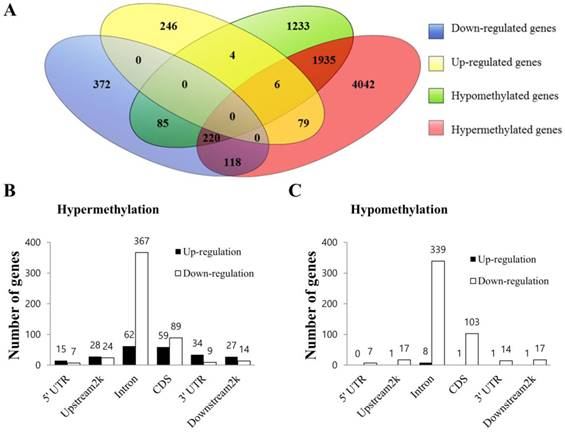
\includegraphics[width=0.8\textwidth]{journal-of-cancer_sample-result}}
%	\caption{یک نمونه نمودار خلاصه برای نمایش نوآوری در نتایج
%		%\cite{kim2016integrated}
%	}
%	\label{fig:sampleDiagram}
%\end{figure}\\
%طبیعتاً به صلاحدید نگارنده، شکل‌ها و نمودار‌ها می توانند در بخش های مختلف، خصوصا فصل
%\ref{chap:results}
%مورد استفاده قرار گیرند.
%
%\subsection{تعریف واژه‌ها (اختیاری)}
%در این قسمت محقق باید واژه‌هایی را که ممکن است برای خواننده آشنا نباشد، تعریف کند.
%
%\subsection{خلاصه فصل‌ها}
%در آخرین قسمتِ فصل اول پایان‌نامه، خلاصه‌ای اشاره‌وار از فصل‌های آتی آورده می‌شود تا خواننده بتواند تصویری واضح از دیگر قسمت‌های پایان‌نامه در ذهن خود ترسیم کند.
%
%\section{جمع‌بندی}
%در این فصل به دو مقولهٔ نحوه استفاده از قالب \پ دانشگاه تهران و نیز ویژگی‌هایی که محتویات فصل اول پایان‌نامه (یعنی مقدمه) باید داشته باشند، پرداخته شد. با توجه به اینکه این راهنما نحوه استفاده از قالب را شرح داده، ملزومات محتوایی هر فصل پایان‌نامه را توضیح می‌دهد و در پیوست‌ها نیز نحوهٔ کار با لاتک را یادآوری خواهد کرد، بنابراین مطالعهٔ کامل آن مقداری وقت شما را خواهد گرفت؛ اما مطمئن باشید از اتلاف وقت شما در ادامه کارتان تا حد زیادی جلوگیری خواهد کرد. در نوشتن متن حاضر سعی شده است علاوه بر ایجاد یک قالب لاتک برای پایان‌نامه‌های دانشگاه تهران، نکات محتوایی هر فصل نیز گوشزد گردد. طبیعتاً برای نگارش پایان‌نامهٔ خود می‌بایست مطالب تمام فصل‌ها را خودتان بازنویسی کنید.
%
%در ادامهٔ این راهنما، تنها فصل‌هایی که یک پایان‌نامه باید داشته باشد و نیز خصوصیات یا ساختاری که محتویات هر فصل باید از آنها برخوردار باشد%
%\footnote{از روی فایل «تمپلیت نگارش و تدوین پایان‌نامه \cite{UTThesisGuide}»}،
%آورده می‌شوند. نهایتاً  در پیوست‌ها، مطالبی در باب یادآوری دستورات لاتک، نحوه نوشتن فرمول‌ها، تعاریف، قضایا، مثال‌ها، درج تصاویر، نمودارها، جداول و الگوریتم‌ها و نیز مدیریت مراجع، آمده است.
%
%همچنین توصیه اکید دارم که رفع خطاهایی که احتمالاً با آنها مواجه می‌شوید را به آخر موکول نفرمایید و به محض برخورد با خطا، آن را اشکال‌زدایی و برطرف نمائید.!
%و
%\verb!% !TeX root=../main.tex
\chapter{پیشینه پژوهش}
%\thispagestyle{empty} 
\section{تولید آزمایه به صورت خودکار}
تولید خودکار آزمایه 
\LTRfootnote{Testcase}
به معنای ایجاد سناریوهای آزمون به صورت خودکار، بدون نیاز به دخالت دستی است. در این روش آزمونگر از تکنیک‌ها و ابزارهای ویژه‌ای استفاده می‌کند تا سناریوهای متنوعی برای آزمون نرم‌افزار تحت آزمون
\LTRfootnote{System Under Test}
 ایجاد کند. مزایای این روش عبارت‌اند از:
\begin{itemize}
	\item \textbf{پوشش گسترده‌تر آزمون:} تولید خودکار آزمایه‌ها، مواردی را پوشش می‌دهد که ممکن است در آزمون‌های دستی نادیده گرفته شوند. این امر به ویژه در آزمون نرم‌افزارهای پیچیده و بزرگ اهمیت بیشتری دارد.
	\item \textbf{افزایش کارایی آزمون:} با خودکارسازی فرآیند تولید آزمایه‌ها، می‌توان تعداد زیادی آزمایه در مدت زمان کوتاهی ایجاد کرد، که این کارایی در فازهای توسعه و نگهداری نرم‌افزار بسیار مفید است.
	\item \textbf{کشف باگ‌های ناشناخته:} تولید خودکار آزمایه‌ها به شناسایی باگ‌هایی کمک می‌کند که ممکن است در سناریوهای پیش‌بینی‌نشده رخ دهند. آزمون‌های تصادفی به خصوص در این زمینه بسیار مؤثر هستند.
	\item \textbf{کاهش دخالت انسانی:} خودکارسازی تولید آزمایه‌ها باعث کاهش خطاهای انسانی می‌شود و دقت و اطمینان آزمون‌ها را افزایش می‌دهد.
\end{itemize}

\section{آزمون تصادفی}
آزمون تصادفی \LTRfootnote{Random Testing} یک روش آزمون نرم‌افزار جعبه سیاه\LTRfootnote{Black Box Testing} است که در آن سیستم تحت آزمون با ورودی‌های تولید شده به صورت تصادفی ارزیابی می‌شود. هدف اصلی آزمون تصادفی، شناسایی اشکالات نرم‌افزار و اطمینان از قابلیت اطمینان و استحکام نرم‌افزار در مواجهه با انواع مختلف سناریوهای ورودی است.
\subsection{فرآیند تولید آزمایه توسط آزمون تصادفی}
فرآیند تولید آزمایه به صورت خودکار توسط روش آزمون تصادفی را می‌توان به صورت زیر ترسیم کرد:

\begin{enumerate}
	\item \textbf{تعریف فضای ورودی\LTRfootnote{Input Domain}:} در این مرحله محدوده و نوع ورودی‌هایی که نرم‌افزار می‌تواند بپذیرد، مشخص می‌گردد. این شامل تعیین دامنه‌های ورودی و محدودیت‌ها برای اطمینان از صحت موارد آزمون تولید شده است.
	\item \textbf{تولید موارد آزمون:} مجموعه‌ای از مقادیر ورودی به صورت تصادفی در داخل فضای ورودی تعریف شده تولید می‌شود. این ورودی‌ها باید طیف گسترده‌ای از سناریوهای ممکن را پوشش دهند تا احتمال کشف اشکالات افزایش یابد.
	\item \textbf{اجرای آزمون:} نرم‌افزار با استفاده از ورودی‌های تولید شده تصادفی اجرا شده و رفتار و خروجی‌های آن برای هر گونه ناهنجاری یا نتایج غیرمنتظره نظارت می‌شود.
	\item \textbf{ارزیابی خروجی‌ها:} خروجی‌های واقعی نرم‌افزار با خروجی‌های مورد انتظار (در صورت موجود بودن) مقایسه می‌شوند تا هر گونه تفاوت شناسایی گردد. در مواردی که خروجی مورد انتظار از پیش تعیین نشده است، از روش‌های اکتشافی یا اوراکل‌ها
		\LTRfootnote{Oracle}
	 برای ارزیابی درستی رفتار سیستم تحت آزمون استفاده می‌شود.
	\item \textbf{شناسایی و تحلیل اشکالات:} هر گونه انحراف یا خرابی که در حین آزمون شناسایی شود، تحلیل می‌گردد تا علل زیربنایی آن تشخیص داده شود.
\end{enumerate}


\subsection{مزایای آزمون تصادفی}
آزمون تصادفی چندین مزیت دارد که آن را به یک تکنیک ارزشمند در آزمون نرم‌افزار تبدیل می‌کند:
\begin{itemize}
	\item \textbf{سادگی:} این روش به سادگی قابل پیاده‌سازی است و نیازی به دانش عمیق از ساختار داخلی نرم‌افزار ندارد. موارد آزمون می‌توانند به صورت خودکار و بدون تلاش دستی، به صورت نامحدود تولید شوند.
	\item \textbf{خودکارسازی:} آزمون تصادفی می‌تواند به طور کامل خودکار شود و امکان آزمون پیوسته و بدون نیاز به نظارت انسانی را فراهم کند. این امر نیاز به دخالت انسانی را کاهش می‌دهد.
	\item \textbf{پوشش گسترده:} با تولید مجموعه‌ای متنوع از ورودی‌های تصادفی، آزمون تصادفی می‌تواند طیف گسترده‌ای از سناریوهای ورودی را پوشش دهد. این امر احتمال کشف اشکالات نادر یا غیرمنتظره‌ای که ممکن است از طریق دیگر روش‌های آزمون نرم‌افزار شناسایی نشوند را افزایش می‌دهد.
\end{itemize}

\subsection{معایب آزمون تصادفی}
با وجود مزایای آن، آزمون تصادفی چندین محدودیت دارد که می‌تواند بر اثربخشی آن تأثیر بگذارد:
\begin{itemize}
	\item \textbf{ناکارآمدی:} این روش می‌تواند از نظر زمان و منابع محاسباتی ناکارآمد باشد. بسیاری از ورودی‌های تولید شده ممکن است موارد آزمون معناداری را تحریک نکنند، که منجر به هدر رفتن تلاش‌ها و منابع استفاده شده جهت آزمون می‌شود.
	\item \textbf{تکرارپذیری:} آزمون تصادفی ممکن است موارد آزمون تکراری تولید کند که ارزش افزوده زیادی ندارند. نبود تمرکز بر نواحی بحرانی می‌تواند منجر به حجم بالای آزمون‌ها با نرخ شناسایی اشکال پایین شود.
	\item \textbf{تمرکز محدود:} آزمون تصادفی نواحی ورودی خاص یا نقاط خرابی بحرانی را اولویت‌بندی نمی‌کند. بنابراین، ممکن است اشکالات مهمی که در نواحی کمتر آزمون شده متمرکز شده‌اند را نادیده بگیرد.
\end{itemize}

%===============================================================================================================

\section{آزمون تصادفی تطبیقی}
آزمون تصادفی تطبیقی \LTRfootnote{Adaptive Random Testing}  با هدف بهبود آزمون تصادفی سنتی به وجود آمد و به ناکارآمدی‌ها و محدودیت‌های آن پرداخت. مفهوم آزمون تصادفی تطبیقی برای افزایش قابلیت‌های شناسایی اشکال آزمون تصادفی، با استفاده از استراتژی‌های تطبیقی که انتخاب موارد آزمون را هدایت می‌کنند، معرفی شد. آزمون تصادفی تطبیقی هدف دارد تا نرخ شناسایی اشکال بهتر را با حفظ مزایای سادگی و خودکارسازی آزمون تصادفی، بیشتر کند.

\subsection{فرضیه اصلی آزمون تصادفی تطبیقی}

توسعه آزمون تصادفی تطبیقی به دلیل نیاز به کاهش تکرارپذیری و ناکارآمدی مرتبط با تولید موارد آزمون به صورت تصادفی خالص به وجود آمد. محققان مشاهده کردند که اشکالات نرم‌افزار تمایل دارند در برخی نواحی فضای ورودی متمرکز شوند و به عبارت دیگر \textbf{نقاط خطا و شکست درون دامنه ورودی به صورت ناحیه‌ای هستند و تمایل به پیوسته بودن دارند.} در نتیجه هر چه تراکم آزمایه‌ها روی دامنه ورودی بیشتر باشد، احتمال کشف خطای جدید بیشتر خواهد بود. آزمون تصادفی تطبیقی از این مشاهده بهره می‌برد و از بازخورد موارد آزمون قبلی برای هدایت تولید موارد آزمون بعدی استفاده می‌کند. به طور کلی، آزمون تصادفی تطبیقی، آزمون تصادفی سنتی را با استفاده از تکنیک‌هایی که توزیع یکنواخت‌تری از موارد آزمون را در سراسر فضای ورودی تضمین می‌کنند، تقویت می‌کند. اصل کلیدی روش آزمون تصادفی تطبیقی این است که حداکثر تنوع موارد آزمون را به دست آورد و به این ترتیب، احتمال شناسایی خطا را افزایش دهد.

\subsection{فرآیند تولید آزمایه توسط آزمون تصادفی تطبیقی}

فرآیند تولید آزمایه به صورت خودکار توسط روش آزمون تصادفی تطبیقی را می‌توان به صورت زیر ترسیم کرد:
\begin{itemize}
	\item \textbf{تولید مجموعه کاندید\LTRfootnote{Candidate Set}:} در این مرحله ابتدایی، یک مجموعه‌ای از آزمایه‌ها با استفاده از روش آزمون تصادفی تولید می‌شود. این آزمایه‌ها به صورت تصادفی روی فضای ورودی تعریف شده از نرم‌افزار ایجاد می‌شوند.
	\item \textbf{انتخاب آزمایه:} از مجموعه کاندید تولید شده، یک آزمایه بر اساس یک استراتژی خاص که منحصراً به روش آزمون تصادفی تطبیقی مربوط است، انتخاب می‌شود. این استراتژی معمولاً به منظور به حداکثر رساندن فاصله آزمایه‌ها در فضای ورودی عمل می‌کند. با انتخاب آزمایه‌هایی که به طور گسترده‌تری پراکنده شده‌اند، آزمون تصادفی تطبیقی سعی دارد که احتمال کشف خطاها را نسبت به آزمون تصادفی سنتی افزایش دهد.
	\item \textbf{تکرار:} آزمایه انتخاب شده به مجموعه آزمایه‌های انتخاب شده \LTRfootnote{Executed Set}اضافه می‌شود و مراحل فوق به صورت تکراری انجام می‌شود. فرآیند تولید یک مجموعه کاندید جدید و انتخاب یک آزمایه ادامه می‌یابد تا زمانی که شرط خاتمه ارضاء شود که برای مثال شرط خاتمه می‌تواند رسیدن به تعداد مشخصی آزمایه باشد.
\end{itemize}
با دنبال کردن این مراحل، آزمون تصادفی تطبیقی تلاش می‌کند تا با تمرکز بر توزیع یکنواخت‌تر آزمایه‌ها، قابلیت کشف خطا را در مقایسه با آزمون تصادفی سنتی بهبود بخشد.

\subsection{مزایای آزمون تصادفی تطبیقی}
آزمون تصادفی تطبیقی چندین مزیت دارد که آن را به جایگزینی برتر برای آزمون تصادفی سنتی تبدیل می‌کند. در ادامه به برخی از این مزیت‌ها اشاره شده است:
\begin{itemize}
	\item \textbf{کاهش تکرارپذیری:} آزمون تصادفی تطبیقی با تولید موارد آزمون متنوع تکرارپذیری را کاهش می‌دهد. این امر ارزش هر مورد آزمون را به حداکثر می‌رساند و تلاش‌های بیهوده آزمون را به حداقل می‌رساند.
	\item \textbf{افزایش کارایی و نرخ شناسایی اشکال بالاتر:}‌ به دنبال کاهش تکرارپذیری موارد آزمون، کارایی روش آزمون تصادفی تطبیقی افزایش می‌یابد و فرآیند آزمون را بهبود می‌بخشد، که این خود منجر به نرخ شناسایی اشکال بالاتر با تعداد آزمایه کمتر می‌شود.
	\item \textbf{پوشش متعادل:} روش آزمون تصادفی تطبیقی، پوشش متعادل‌تری از فضای ورودی را به دست می‌آورد و خطر نادیده گرفتن نواحی مهم را کاهش می‌دهد. این پوشش جامع، استحکام کلی نرم‌افزار را افزایش می‌دهد.
	\item \textbf{بهینه‌سازی منابع:} با بهبود کارایی تولید موارد آزمون، آزمون تصادفی تطبیقی از منابع محاسباتی و زمانی بهینه استفاده می‌کند. این امر آزمون تصادفی تطبیقی را به یک راه‌حل عملی و مقیاس‌پذیر برای آزمون نرم‌افزار در مقیاس بزرگ تبدیل می‌کند.
\end{itemize}

\subsection{سربار محاسباتی پیاده سازی آزمون تصادفی تطبیقی}
در مرحله انتخاب آزمایه از فرآیند پیاده‌سازی روش آزمون تصادفی تطبیقی، لازم است که فاصله بین هر آزمایه درون مجموعه کاندید و هر آزمایه درون مجموعه آزمایه‌های انتخاب‌شده در مراحل قبلی محاسبه شود. آزمایه‌ای که بیشترین فاصله را با مجموعه آزمایه‌های انتخاب‌شده دارد، انتخاب می‌شود. در این مرحله، تعداد محاسبات فاصله باید به اندازه‌ی (تعداد آزمایه‌های درون مجموعه کاندید × تعداد آزمایه‌های درون مجموعه آزمایه‌های انتخاب‌شده) انجام شود. با افزایش تعداد اعضای مجموعه آزمایه‌های انتخاب‌شده در هر بار تکرار فرآیند، سربار محاسباتی الگوریتم آزمون تصادفی تطبیقی افزایش می‌یابد. همچنین، تعداد اعضای درون مجموعه کاندید نیز تأثیر مستقیمی بر افزایش سربار محاسباتی الگوریتم دارد. در ادامه، استراتژی‌هایی که تاکنون برای کاهش اندازه مجموعه کاندید، کاهش تعداد آزمایه‌های درون مجموعه آزمایه‌های انتخاب‌شده در مراحل قبلی الگوریتم، و در نهایت کاهش تعداد محاسبات فاصله ارائه شده‌اند، شرح داده می‌شود.

\subsubsection{اندازه مجموعه کاندید ثابت}
اولین و پرکاربردترین استراتژی پیاده‌سازی الگوریتم آزمون تصادفی تطبیقی، استراتژی "انتخاب آزمایه از مجموعه کاندید با اندازه ثابت\LTRfootnote{Fixed Sized Candidate Set (FSCS)}" است. در این استراتژی، که توسط [نام پژوهشگر/منبع] ارائه شده است، اندازه مجموعه کاندید در کل روند اجرای الگوریتم ثابت در نظر گرفته می‌شود. بهترین مقدار برای اندازه مجموعه کاندید طبق پژوهش [نام پژوهشگر/منبع] برابر با ۱۰ اعلام شده است. البته، هر چه اندازه مجموعه کاندید را افزایش دهیم، این امر می‌تواند بر اثربخشی آزمایه‌های نهایی تأثیر داشته باشد. اما بر اساس این پژوهش، هنگامی که اندازه مجموعه کاندید از ۱۰ بیشتر باشد، میزان افزایش اثربخشی مجموعه آزمایه‌ها خیلی قابل توجه نیست.

\subsubsection{بزرگ شدن فضای آزمون در آزمون تصادفی تطبیقی}
یکی از چالش‌های اصلی و مهم در آزمون تصادفی تطبیقی، بزرگ شدن فضای آزمون است. با افزایش تعداد آزمایه‌های انتخاب شده، محاسبه فاصله هر آزمایه جدید با آزمایه‌های قبلی زمان‌بر و ناکارآمد می‌شود. این مسئله باعث افزایش پیچیدگی محاسباتی و کاهش کارایی فرآیند آزمون می‌شود. برای مقابله با این مشکل، استراتژی‌های مختلفی ارائه شده‌اند که هدف آن‌ها کاهش فضای آزمون و بهبود کارایی تولید آزمایه‌ها است.
\begin{itemize}
	\item \textbf{استراتژی فراموشی\LTRfootnote{Forgetting Strategy}:} استراتژی فراموشی به منظور مدیریت فضای آزمون و جلوگیری از بزرگ شدن بیش از حد آن استفاده می‌شود. در این روش، زمانی که مجموعه آزمایه‌های از قبل انتخاب‌شده به توزیع یکنواخت مناسبی می‌رسند، این مجموعه پاک می‌شود. با این کار، فقط آزمایه‌های جدیدتر و مرتبط‌تر در فرآیند محاسبه فاصله‌ها لحاظ می‌شوند. در این استراتژی با پاک کردن آزمایه‌های قدیمی‌تر، حجم داده‌های مورد نیاز برای محاسبه فاصله‌ها کاهش می‌یابد و محاسبات سریع‌تر و کارآمدتر انجام می‌شود. البته، احتمال از دست رفتن اطلاعات مفید از آزمایه‌های قبلی وجود دارد و همچنین معیارهای فراموشی باید به دقت تنظیم شوند تا بهترین نتیجه حاصل شود.
	
	\item \textbf{خوشه‌بندی \lr{K}-مرکز\LTRfootnote{K-means Clustering Strategy}:} خوشه‌بندی \lr{K}-مرکز یکی دیگر از استراتژی‌های کاهش فضای آزمون است. در این روش، آزمایه‌های انتخاب‌شده به خوشه‌هایی تقسیم می‌شوند و هر خوشه با یک نماینده (میانگین) که مرکز خوشه است، مشخص می‌شود. برای انتخاب آزمایه جدید، فاصله بین آزمایه‌های کاندید و نمایندگان خوشه‌ها محاسبه می‌شود. این استراتژی علاوه بر کاهش تعداد محاسبات فاصله، باعث مدیریت بهتر فضای آزمون می‌شود و فضای آزمون به صورت خوشه‌بندی‌شده نگهداری می‌شود. با این حال، این روش ممکن است پیچیدگی اجرای الگوریتم را افزایش دهد و تعیین تعداد خوشه‌ها (\lr{K}) باید به دقت انجام شود تا بهترین نتیجه حاصل شود.
	
	\item \textbf{استراتژی شبکه‌بندی\LTRfootnote{Grid Strategy}:} در این روش، فضای ورودی به سلول‌های کوچکتری تقسیم می‌شود. آزمایه‌های انتخاب‌شده در هر سلول ذخیره می‌شوند و برای انتخاب آزمایه جدید، فقط سلول‌های مجاور مورد بررسی قرار می‌گیرند. این استراتژی علاوه بر کاهش تعداد محاسبات فاصله، باعث مدیریت بهتر فضای آزمون می‌شود و فضای آزمون به صورت شبکه‌بندی‌شده نگهداری می‌شود. با این حال، این روش به پیاده‌سازی دقیق شبکه‌بندی نیاز دارد و اندازه سلول‌ها باید به دقت تنظیم شود تا بهترین نتیجه حاصل شود.

\end{itemize}

\subsection{اولین پیاده‌سازی روش آزمون تصادفی تطبیقی}
اولین پیاده‌سازی روش آزمون تصادفی تطبیقی روی برنامه‌هایی با ورودی عددی\LTRfootnote{Numerical Input Domain} انجام شد. در این پیاده‌سازی، هر آزمایه که مجموعه‌ای از ورودی‌های عددی بود، به صورت یک نقطه درون یک فضای چندبعدی (تعداد ابعاد برابر با تعداد ورودی‌ها) مدل‌سازی شد. در ادامه، این الگوریتم روی یک مثال ساده بررسی می‌شود.

فرض کنید که یک برنامه به نام \lr{Sum} دارید که دو عدد به عنوان ورودی دریافت کرده و حاصل جمع آن‌ها را برمی‌گرداند. در این الگوریتم، آزمایه‌های این برنامه روی یک فضای دوبعدی به صورت نقطه مدل خواهند شد (برای مثال، آزمایه با ورودی‌های ۱۰ و ۱۵ در فضای ورودی دوبعدی نقطه \lr{(10,15)} را تشکیل می‌دهد) و فاصله بین آن‌ها، همان فاصله اقلیدسی\LTRfootnote{Euclidean distance} بین دو نقطه در نظر گرفته می‌شود.

این روش با روش آزمون تصادفی سنتی روی چند برنامه مختلف با ورودی عددی پیاده‌سازی شد و نتایج نشان داد که این روش از روش آزمون تصادفی سنتی کارایی و عملکرد بهتری دارد.

اما مهم‌ترین مشکل این روش این بود که تنها روی برنامه‌هایی با ورودی عددی قابل پیاده‌سازی بود. با این حال، این مسئله باعث شد که زمینه پژوهشی جدیدی برای محققان ایجاد شود تا راهکاری برای محاسبه فاصله بین دو آزمایه با ورودی‌های غیرعددی\LTRfootnote{Obejctive} ارائه دهند. در اکثر راهکارهای ارائه‌شده، تلاش بر این بوده که هر آزمایه را به عنوان یک نقطه در یک یا چند فضای چندبعدی مدل کنند و سپس با استفاده از محاسبات ریاضی رایج برای محاسبه فاصله در فضاهای چندبعدی، مانند فاصله اقلیدسی، فاصله بین دو نقطه را به دست آورده و به عنوان فاصله بین دو آزمایه ارائه دهند.

\subsection{آخرین ایده پیاده‌سازی ارائه شده برای روش آزمون تصادفی تطبیقی}
آخرین روشی که تاکنون در این حوزه توسط [نام پژوهشگر/منبع] ارائه شده است، شامل روش‌های \lr{WTClustering-ART} و \lr{TFClustering-ART} می‌باشد. در ادامه به بررسی دقیق ساختار و نحوه کارکرد هر کدام از این روش‌ها پرداخته شده است.

\subsubsection{تبدیل فرکانس }
کاهوچی و همکارانش روش‌هایی بر مبنای تبدیل فرکانس\LTRfootnote{Frequency Transform}، که قبلاً برای تبدیل رشته‌ها در جستجوی تشابه رشته‌ها استفاده می‌شد، پیشنهاد کردند. این روش یک رشته با طول تعریف‌شده را با تعداد دفعات هر کاراکتر در رشته به یک بردار فرکانس\LTRfootnote{Frequency Vector} تبدیل می‌کند. تعریف دقیق بردار فرکانس در ادامه آورده شده است.

\begin{itemize}
	\item \textbf{بردار فرکانس:}
	فرض کنید که \(\Sigma = \{m_1, m_2, \dots, m_n\}\) لیست توابع در یک برنامه فرضی باشد و \(s\) ترتیب فراخوانی توابع توسط آزمایه \(t\) باشد. حال بردار فرکانس به صورت 
	\(f(s) = \{f_1, f_2, \dots, f_n\}\)
	 تعریف خواهد شد که \(f_i\) تعداد دفعاتی است که تابع \(m_i\) در ترتیب فراخوانی توابع (\(s\)) حضور دارد.
	
	برای مثال فرض کنید که \(\Sigma = \{a, b, c, d, e\}\) و \(s = abddc\) ترتیب فراخوانی توابع در حین اجرای آزمایه \(t\) باشد. در این وضعیت، تابع \(a\) یک بار، \(b\) یک بار، \(c\) صفر بار، \(d\) دو بار و \(e\) یک بار فراخوانی شده است. در نتیجه:
	\[
	f(s) = \{1, 1, 0, 2, 1\}
	\]
	
	حال با توجه به اینکه هر آزمایه به یک لیست عددی با طول \(n\) (یک نقطه در فضای \(n\) بعدی) تبدیل شده است، اکنون می‌توان به سادگی فاصله بین آزمایه‌ها را با استفاده از محاسبه فاصله بین نقطه‌های متناظر آزمایه‌ها به دست آورد.
	
\end{itemize}

\subsubsection{تبدیل موجک}
اگرچه تبدیل فرکانس می‌تواند به راحتی آزمایه‌های شیء‌گرا را به بردارهایی برای اندازه‌گیری عدم تشابه تبدیل کند، اما فقط بر فرکانس فراخوانی توابع تمرکز می‌کند و به ترتیب فراخوانی توابع اهمیتی نمی‌دهد. از آنجایی که ترتیب واقعی فراخوانی توابع معمولاً بر نتایج اجرا تأثیر می‌گذارد، عدم تشابه محاسبه‌شده رضایت‌بخش نیست.

برای مثال، فرض کنید \(\Sigma = \{a, b, c, d, e\}\) و \(s_1 = acbe\) ترتیب فراخوانی توابع در آزمایه \(t_1\) و \(s_2 = bcae\) ترتیب فراخوانی توابع در آزمایه \(t_2\) باشد. بعد از انجام تبدیل فرکانس، دو بردار فرکانس\\ \(f(s_1) = f(s_2) = \{1, 1, 1, 0, 1\}\) به دست خواهد آمد. فاصله بین آزمایه \(t_1\) و \(t_2\) با توجه به مقایسه بردارهای فرکانس این دو آزمایه صفر است، در حالی که ترتیب فراخوانی توابع در دو آزمایه کاملاً یکسان نیست.

از این رو، روش تبدیل موجک در این مقاله ارائه شد که علاوه بر تعداد فراخوانی هر تابع، به ترتیب فراخوانی توابع نیز تا حدی اهمیت می‌دهد. تبدیل موجک\LTRfootnote{Wavelet Transform} ابزاری ریاضی است که برای تجزیه و تحلیل سیگنال‌ها و داده‌ها در حوزه زمان و فرکانس استفاده می‌شود. در این مقاله، از تبدیل موجک برای اندازه‌گیری عدم تشابه بین تست‌ کیس‌های شیءگرا استفاده می‌شود. این معیار با تجزیه و تحلیل سیگنال‌های مربوط به ویژگی‌های آزمایه‌ها، میزان تفاوت بین آن‌ها را محاسبه می‌کند. در روش
 \lr{ART\_WTClustering} 
 از موجک هار \LTRfootnote{Haar Wavelet} برای مدل‌سازی اطلاعات فرکانس و اطلاعات ترتیب فراخوانی توابع استفاده شده است. در ادامه، معیار تبدیل موجک با مثال توضیح داده شده است.

\begin{itemize}
	\item \textbf{تعریف تبدیل موجک آزمایه:}
فرض کنید \(s = m_1 m_2 \dots m_j\) ترتیب فراخوانی توابع باشد. \(s_1\) یک زیررشته از \(s\) است که حاوی نیمه اول عناصر \(s\) است و \(s_2\) یک زیررشته دیگر از \(s\) است که حاوی نیمه دوم عناصر \(s\) است. تبدیل موجک \(s\) به صورت \(W(s) = [A, B]\) تعریف می‌شود که \(A = f(s)\) و \(B = B_1 - B_2\) که \(B_1 = f(s_1)\) و \(B_2 = f(s_2)\) است.

برای مثال فرض کنید که \(\Sigma = \{a, b, c, d, e\}\) و \(s = abdde\) ترتیب فراخوانی توابع در حین اجرای آزمایه \(t\) باشد. حال مقادیر \(A\) , \(B\) و \(W(s)\) به صورت زیر محاسبه خواهند شد:
\begin{align*}
	A = f(s) &= \{1, 1, 0, 2, 1\} \\
	s_1 = ab \quad & \Rightarrow \quad B_1 = \{1, 1, 0, 0, 0\} \\
	s_2 = dde \quad &\Rightarrow \quad B_2 = \{0, 0, 0, 2, 1\} \\
	B = B_1 - B_2 \quad &\Rightarrow \quad B = \{1, 1, 0, -2, -1\} \\
	W(s) = [A, B] \quad &\Rightarrow \quad W(s) = \left[\{1, 1, 0, 2, 1\}, \{1, 1, 0, -2, -1\}\right]
\end{align*}

\item \textbf{محاسبه فاصله بین آزمایه‌‌ها:}
فرض کنید \(\Sigma = \{m_1, m_2, \dots, m_n\}\) لیست توابع درون یک برنامه فرضی باشد. اگر \(s_1\) ترتیب فراخوانی توابع توسط آزمایه \(t_1\) و \(s_2\) ترتیب فراخوانی توابع توسط آزمایه \(t_2\) باشد، آنگاه \(W(s_1) = [A_1, B_1]\) و \(W(s_2) = [A_2, B_2]\) خواهد بود که \(A_1 = \{A_{11}, A_{12}, \dots, A_{1n}\}\) و \(B_1 = \{B_{11}, B_{12}, \dots, B_{1n}\}\) و \(A_2 = \{A_{21}, A_{22}, \dots, A_{2n}\}\) و \(B_2 = \{B_{21}, B_{22}, \dots, B_{2n}\}\) که فاصله \(WT\_D\) بین این دو آزمایه به صورت زیر محاسبه خواهد شد:
\[
WT\_D(t_1, t_2) = \sqrt{\sum_{i=1}^{n} (A_{1i} - A_{2i})^2} + \sqrt{\sum_{i=1}^{n} (B_{1i} - B_{2i})^2}
\]


\end{itemize}

\subsubsection{تبدیل فرکانس سه‌بخشی}
تا حدی، استفاده مستقیم از تبدیل موجک برای آزمایه‌های شیءگرا نامناسب است. دلیل اصلی این است که، اگرچه دنباله فراخوانی توابع را به دو قسمت تقسیم می‌کند و آنها را حفظ می‌کند، اما تنها تفریق نیمه اول و دوم این دنباله نمی‌تواند تفاوت بین توالی فراخوانی توابع را نمایش دهد. برای پرداختن به این موضوع، در این مقاله پیشنهاد شده است که از تبدیل فرکانس سه‌بخشی \LTRfootnote{Trisection Frequency Conversion (TFC)} استفاده شود. این معیار نه تنها به تعداد فراخوانی هر تابع در حین اجرای آزمایه‌ها توجه دارد بلکه ترتیب فراخوانی توابع در حین اجرای آزمایه‌های مختلف نیز اهمیت دارد.

\begin{itemize}

\item \textbf{تعریف معیار تبدیل فرکانس سه‌بخشی:}
فرض کنید که \(s = m_1 m_2 \dots m_j\) ترتیب فراخوانی توابع در حین اجرای آزمایه \(t\) باشد و \(s_1\) نیمه اول \(s\) و \(s_2\) نیمه دوم \(s\) باشد. معیار تبدیل فرکانس سه‌بخشی برای \(s\) به صورت \(TF(s) = [A, B, C]\) نمایش داده می‌شود که \(A = f(s)\)، \(B = f(s_1)\) و \(C = f(s_2)\) است.

\item \textbf{محاسبه فاصله بین آزمایه‌‌ها:}

فرض کنید \(\Sigma = \{m_1, m_2, \dots, m_n\}\) لیست توابع در یک برنامه فرضی باشد. یک آزمایه \(t_1\) با دنباله فراخوانی توابع \(s_1\) و یک آزمایه \(t_2\) با دنباله فراخوانی توابع \(s_2\) را در نظر بگیرید. فرض کنید\\ \(TF(s_1) = [A_1, B_1, C_1]\) و \(TF(s_2) = [A_2, B_2, C_2]\) که در آن \(A_1 = \{A_{11}, A_{12}, \dots, A_{1n}\}\)، \(B_1 = \{B_{11}, B_{12}, \dots, B_{1n}\}\)، \(C_1 = \{C_{11}, C_{12}, \dots, C_{1n}\}\)، \(A_2 = \{A_{21}, A_{22}, \dots, A_{2n}\}\)، \(B_2 = \{B_{21}, B_{22}, \dots, B_{2n}\}\)، و \(C_2 = \{C_{21}, C_{22}, \dots, C_{2n}\}\). تفاوت ترتیب بین \(s_1\) و \(s_2\) به صورت \(\sum_{i=1}^{j} \left(1 - \delta_{s_{1i} s_{2i}}\right)\) تعریف می‌شود، که \(\delta_{s_{1i} s_{2i}}\) نماد دلتای کرونکر استاندارد است، به طوری که اگر \(s_{1i} = s_{2i}\) باشد آنگاه \(\delta_{s_{1i} s_{2i}} = 1\) و در غیر اینصورت \(\delta_{s_{1i} s_{2i}} = 0\). فاصله \(TFC\)  یا \(TFC\_D\) بین این دو آزمایه به صورت زیر تعریف می‌شود:

\[
TFC\_D(t_1, t_2) = \sqrt{\sum_{i=1}^{n} (A_{1i} - A_{2i})^2} + \sqrt{\sum_{i=1}^{n} (B_{1i} - B_{2i})^2}
\]
\[
+ \sqrt{\sum_{i=1}^{n} (C_{1i} - C_{2i})^2} + \sum_{i=1}^{n} \left(1 - \delta_{s_{1i} s_{2i}}\right)
\quad
\]

\end{itemize}

\subsubsection{مقایسه بین \(TFC\_D\) و \(WT\_D\):}
در اینجا به بررسی تفاوت‌های \(WT\_D\) و \(TFC\_D\) در یک مثال پرداخته شده است. دو آزمایه \(t_1\) و \(t_2\) را در نظر بگیرید که ترتیب فراخوانی توابع توسط این دو آزمایه به صورت \(s_1 = abce\) و \(s_2 = abec\) است که \(s_{11} = ab\)، \(s_{12} = ce\)، \(s_{21} = ab\) و \(s_{22} = ec\) است. در نتیجه:

\begin{align*}
	W(s_1) &= \left[\langle 1, 1, 1, 0, 1 \rangle, \langle 1, 1, -1, 0, -1 \rangle \right] \\
	W(s_2) &= \left[\langle 1, 1, 1, 0, 1 \rangle, \langle 1, 1, -1, 0, -1 \rangle \right]
\end{align*}

است و در نتیجه \({WT\_D}(s_1, s_2)\) برابر است با:

\[
WT\_D(s_1, s_2) = \sqrt{0^2 + 0^2 + 0^2 + 0^2 + 0^2} + \sqrt{0^2 + 0^2 + 0^2 + 0^2 + 0^2} = 0
\]
\textbf{}
از طرفی با توجه به تعریف \(TF(s_i)\) مقادیر \(TF(s_1)\) و \(TF(s_2)\) و \(TFC\_D(s_1, s_2)\) به صورت زیر محاسبه می‌شوند:
\[
TF(s_1) = \left[\langle 1, 1, 1, 0, 1 \rangle, \langle 1, 1, 0, 0, 0 \rangle, \langle 0, 0, 1, 0, 1 \rangle\right]
\]
\[
TF(s_2) = \left[\langle 1, 1, 1, 0, 1 \rangle, \langle 1, 1, 0, 0, 0 \rangle, \langle 0, 0, 1, 0, 1 \rangle\right]
\]

\(TFC\_D(s_1, s_2)\) به صورت زیر محاسبه می‌شود:

\begin{align*}
	TFC\_D(s_1, s_2) &= \sqrt{0^2 + 0^2 + 0^2 + 0^2 + 0^2} + \sqrt{0^2 + 0^2 + 0^2 + 0^2 + 0^2} \\
	&\quad + \sqrt{0^2 + 0^2 + 0^2 + 0^2 + 0^2} + \sum_{i=1}^{j} \left(1 - \delta_{s_{1i}s_{2i}}\right)
\end{align*}

که

\[
\sum_{i=1}^{j} \left(1 - \delta_{s_{1i}s_{2i}}\right) = (1-1) + (1-1)  + (1-0)  + (1-0) = 2
\]

بنابراین:

\[
TFC\_D(s_1, s_2) = 0 + 0 + 0 + 2 = 2 
\]

همانطور که مشاهده کردید،‌ فاصله \(TFC\) در این مثال نسبت به فاصله \(ٌُWT\)  به ترتیب فراخوانی توابع توسط آزمایه‌ها اهمیت بیشتری می دهد.


\newpage

	\begin{tikzpicture}[node distance=2.5cm]
		
		\node (start) [startstop] {\rl{به صورت تصادفی اولین مورد آزمایشی شئ‌گرا را ایجاد کرده و اجرا کنید}};
		\node (decision) [decision, below of=start, yshift=-1cm] {\rl{شرط خاتمه}};
		\node (output) [startstop, right of=decision, xshift=4cm] {\rl{خروجی آزمایه‌های تولید شده}};
		\node (process1) [process, below of=decision, yshift=-1cm] {\rl{اضافه کردن این آزمایه به مجموعه آزمایه‌های انتخاب شده در مراحل قبلی الگوریتم}};
		\node (process2) [process, below of=process1, yshift=-1cm] {\rl{تولید ۱۰ آزمایه شئ‌گرا جدید به عنوان مجموعه کاندید}};
		
		\node (process3) [process, below of=process2, yshift=-1cm, xshift=0.5cm, text width=7cm] {\rl{خوشه‌بندی مجموعه آزمایه‌های از قبل انتخاب شده به \rl{K} خوشه}};
		\node (process4) [process, below of=process3, yshift=-0.5cm] {\rl{تعیین نماینده هر خوشه برای ارزیابی آزمایه‌های کاندید}};
		\node (process5) [process, below of=process4, yshift=-0.5cm] {Select the candidate which has the smallest distance with the subset};
		
		\draw [arrow] (start) -- (decision);
		\draw [arrow] (decision) -- node[anchor=east] {No} (process1);
		\draw [arrow] (decision) -- node[anchor=north] {Yes} (output);
		\draw [arrow] (process1) -- (process2);
		\draw [arrow] (process2) -- (process3);
		\draw [arrow] (process3) -- (process4);
		\draw [arrow] (process4) -- (process5);
%		\draw [arrow] (process5.east) -| ++(4,0) |- (decision.east);
		
		% Adding labels ①, ②, ③
%		\node[draw=none, fill=none] at ($(process2)!0.5!(process3)$) {\textcircled{1}};
%		\node[draw=none, fill=none] at ($(process3)!0.5!(process4)$) {\textcircled{2}};
%		\node[draw=none, fill=none] at ($(process4)!0.5!(process5)$) {\textcircled{3}};
		
	\end{tikzpicture}



\subsection{روش‌های مختلف انتخاب آزمایه بر اساس فاصله}


\subsection{نقطه اشتراک اکثر روش‌های پیاده‌سازی الگوریتم آزمون تصادفی تطبیقی}

\section{روش تقسیم‌بندی فضای ورودی}

\subsection{فرآیند تولید آزمایه توسط روش تقسیم‌بندی فضای ورودی}

%===============================================================================================================




%
%
%
%\newpage
%\section{مقدمه}
%هدف از این فصل که با عنوان‌های  «مروری بر ادبیات موضوع%
%\LTRfootnote{Literature Review}»،
%«مروری بر منابع» و یا «مروری بر پیشینه تحقیق%
%\LTRfootnote{Background Research}»
%معرفی می‌شود، بررسی و طبقه‌بندی یافته‌های تحقیقات دیگر محققان در سطح دنیا و تعیین و شناسایی خلأهای تحقیقاتی است. آنچه را که تحقیق شما به دانش موجود اضافه می‌کند، مشخص کنید. طرح پیشینه تحقیق%
%\LTRfootnote{Background Information}
%یک مرور محققانه است و تا آنجا باید پیش برود که پیش‌زمینهٔ تاریخی مناسبی از تحقیق را بیان کند و جایگاه تحقیق فعلی را در میان آثار پیشین نشان دهد. برای این منظور منابع مرتبط با تحقیق را بررسی کنید، البته نه آنچنان گسترده که کل پیشینه تاریخی بحث را در برگیرد. برای نوشتن این بخش:
%\begin{itemize}
%	\item
%	دانستنی‌های موجود و پیش‌زمینهٔ تاریخی و وضعیت کنونی موضوع را چنان بیان کنید که خواننده بدون مراجعه به منابع پیشین، نتایج حاصل از مطالعات قبلی را درک و ارزیابی کند.
%	\item
%	نشان دهید که بر موضوع احاطه دارید. پرسش تحقیق را همراه بحث و جدل‌ها و مسائل مطرح شده بیان کنید و مهم‌ترین تحقیق‌های انجام شده در این زمینه را معرفی نمائید.
%	\item
%	ابتدا مطالب عمومی‌تر و سپس پژوهش‌های مشابه با کار خود را معرفی کرده و نشان دهید که تحقیق شما از چه جنبه‌ای با کار دیگران تشابه یا تفاوت دارد.
%	\item
%	اگر کارهای قبلی را خلاصه کرده‌اید، از پرداختن به جزئیات غیرضروری بپرهیزید. در عوض، بر یافته‌ها و مسائل روش‌شناختی مرتبط و نتایج اصلی تأکید کنید و اگر بررسی‌ها و منابع مروری عمومی دربارهٔ موضوع موجود است، خواننده را به آنها ارجاع دهید.
%\end{itemize}
%
%\section{تعاریف، اصول و مبانی نظری}
%این قسمت ارائهٔ خلاصه‌ای از دانش کلاسیک موضوع است. این بخش الزامی نیست و بستگی به نظر استاد راهنما دارد.
%
%\section{مروری بر ادبیات موضوع}
%در این قسمت باید به کارهای مشابه دیگران در گذشته اشاره کرد و وزن بیشتر این قسمت بهتر است به مقالات ژورنالی سال‌های اخیر (۲ تا ۳ سال) تخصیص داده شود. به نتایج کارهای دیگران با ذکر دقیق مراجع باید اشاره شده و جایگاه و تفاوت تحقیق شما نیز با کارهای دیگران مشخص شود. استفاده از مقالات ژورنال‌های معتبر در دو یا سه سال اخیر، می‌تواند به اعتبار کار شما بیافزاید.
%
%\section{نتیجه‌گیری}
%‌در نتیجه‌گیری آخر این فصل، با توجه به بررسی انجام شده بر روی مراجع تحقیق، بخش‌های قابل گسترش و تحقیق در آن حیطه و چشم‌اندازهای تحقیق مورد بررسی قرار می‌گیرند.	در برخی از تحقیقات، نتیجه نهایی فصل روش تحقیق، ارائهٔ یک چارچوب کار تحقیقی 
%\lr{(research framework)}
است.!
%را در فایل 
%\lr{main.tex}،
%غیرفعال%
%\footnote{
%برای غیرفعال کردن یک دستور، کافی است در ابتدای آن، علامت درصد انگلیسی (\%) بگذارید.
%}
% کنید. در غیر این صورت، ابتدا مطالب دو فصل اول پردازش شده و سپس مطالب فصل ۳ پردازش می‌شود که این کار باعث طولانی شدن زمان پردازش می‌گردد. هر زمان که خروجی کل \پ را خواستید، تمام فصل‌ها را دوباره در
%\lr{main.tex}
%فعال نمائید.
%بدیهتاً لازم نیست فصل‌های \پ را به ترتیب تایپ کنید. مثلاً می‌توانید ابتدا مطالب فصل ۳ را تایپ نموده و سپس مطالب فصل ۱ را تایپ کنید. 
%\subsubsection{مراجع}
%برای وارد کردن مراجع \پ کافی است فایل 
%\lr{MyReferences.bib}
%را باز کرده و مراجع خود را به شکل اقلام نمونهٔ داخل آن، وارد کنید.  سپس از \lr{bibtex} برای تولید مراجع با قالب مناسب استفاده نمائید. برای توضیحات بیشتر بخش \ref{Sec:Ref} از پیوست \ref{app:latexIntro} و نیز پیوست \ref{app:refMan} را ببینید.
%
%\subsubsection{واژه‌نامه فارسی به انگلیسی و برعکس}
%برای وارد کردن معادل فارسی اصطلاحات لاتین در متن و تهیه فهرست واژه‌نامه از آنها، از بستهٔ
%\lr{glossaries}
%و نرم‌افزار
%\lr{xindy}
%استفاده می‌شود. بدین منظور کافی است اصطلاحات لاتین و ترجمهٔ آنها را در فایل
%\lr{words.tex}
%وارد کرده و هر جای متن که خواستید با دستورات
%\verb|gls{label}|
%یا \verb|glspl{label}|
%معادل فارسی مفرد یا جمع یک اصطلاح را بیاورید.
%
%مثلا در اینجا، واژهٔ
%«\gls{Action}»
%برای بار اول و دوباره
%«\gls{Action}»
%برای بار دوم در متن ظاهر شده است.
%جهت توضیحات بیشتر به پیوست
%\ref{app:refMan}
%مراجعه کنید.
%\subsubsection{نمایه}
%برای وارد کردن نمایه، باید از 
%\lr{xindy}
%استفاده کنید. 
%%زیرا 
%%\lr{MakeIndex}
%%با حروف «گ»، «چ»، «پ»، «ژ» و «ک» مشکل دارد و ترتیب الفبایی این حروف را رعایت نمی‌کند. همچنین، فاصله بین هر گروه از کلمات در 
%%\lr{MakeIndex}،
%%به درستی رعایت نمی‌شود که باعث زشت شدن حروف‌چینی این قسمت می‌شود. 
%راهنمای چگونگی کار با 
%\lr{xindy} 
%را می‌توانید در ویکی پارسی‌لاتک و یا مثالهای موجود در دی‌وی‌دی «مجموعه پارسی‌لاتک»، پیدا کنید.
%
%\subsection{اگر سوالی داشتم، از کی بپرسم؟}
%برای پرسیدن سوال‌های خود موقع حروف‌چینی با زی‌پرشین، می‌توانید به
%\href{http://qa.parsilatex.com}{سایت پرسش و پاسخ پارسی‌لاتک}%
%\LTRfootnote{http://qa.parsilatex.com}
%یا
%\href{http://forum.parsilatex.com}{بایگانی تالارگفتگوی قدیمی پارسی‌لاتک}%
%\LTRfootnote{http://forum.parsilatex.com}
%مراجعه کنید. شما هم می‌توانید روزی به سوال‌های دیگران در اینترنت جواب دهید.
%بستهٔ زی‌پرشین و بسیاری از بسته‌های مرتبط با آن مانند
%\lr{bidi} و
%\lr{Persian-bib}،
%مجموعه پارسی‌لاتک، مثالهای مختلف موجود در آن، قالب پایان‌نامه دانشگاههای مختلف و سایت پارسی‌لاتک همه به صورت داوطلبانه توسط افراد گروه پارسی‌لاتک و گروه
%\lr{Persian TeX}
%و بدون هیچ کمک مالی انجام شده‌اند. کار اصلی نوشتن و توسعه زی‌پرشین توسط آقای وفا خلیقی انجام شده است که این کار بزرگ را به انجام رساندند.
%اگر مایل به کمک به گروه پارسی‌لاتک هستید به سایت این گروه مراجعه فرمایید:
%\begin{center}
%	\url{http://www.parsilatex.com}
%\end{center}
%
%\section{محتویات فصل اول یک پایان‌نامه}
%فصل اول یک پایان‌نامه باید به مقدمه یا کلیات تحقیق بپردازد.
%هدف از فصل مقدمه%
%\LTRfootnote{Introduction}،
%شرح مختصر مسأله تحقیق، اهمیت و انگیزه محقق از پرداختن به آن موضوع، بهمراه اشاره‌ای کوتاه به روش و مراحل تحقیق است. مقدمه، اولین فصل از ساختار اصلی \پ بوده و زمینه اطلاعاتی لازم را برای خواننده فراهم می‌آورد. در طول مقدمه باید سعی شود موضوع تحقیق با زبانی روشن، ساده و بطور عمیق و هدفمند به خواننده معرفی شود. این فصل باید خواننده را مجذوب و اهمیت موضوع تحقیق را آشکار سازد. در مقدمه باید با ارائهٔ سوابق، شواهد تحقیقی و اطلاعات موجود (با ذکر منبع) با روشی منظم، منطقی و هدف‌دار، خواننده را جهت داد و به سوی راه حل مورد نظر هدایت کرد. مقدمه مناسب‌ترین جا برای ارائهٔ اختصارات و بعضی توضیحات کلی است، توضیحاتی که شاید نتوان در مباحث دیگر آنها را شرح داد.
%
%مقدمه، یکی از ارکان اساسی و اصلی پایان نامه است که مهمترین قسمت‌های آن عبارتند از: 
%
%\subsection{عنوان تحقیق} 
%باید شناختی دقیق و روشن از حوزهٔ موضوع تحقیق را عرضه دارد و خالی از هرگونه ابهام و پیچیدگی باشد.
%
%\subsection{مسأله تحقیق}
%وظیفه اصلی مقدمه بیان این مطلب به خواننده است که چرا انجام تحقیق را به عهده گرفته‌اید. اگر دلیل شما برای انجام این کار پاسخگویی به سؤال مورد علاقه‌تان است، با مشکل زیادی روبه‌رو نخواهید بود. یکی از بهترین روش‌ها برای نوشتن مقدمهٔ یک پایان‌نامه، طرح پرسش یا پرسش‌هایی مهم و اساسی است که کار تحقیقاتی شما از آغاز تا پایان قصد پاسخ دادن به آن را دارد. گاهی می‌توانید ابتدا اهمیت موضوع را بیان و سپس پرسش خود را در آن موضوع مطرح کنید.
%
%\subsection{تاریخچه‌ای از موضوع تحقیق}
%به طور کلی تشریح روندهای تحقیقاتی در محدودهٔ مورد مطالعه، مستلزم ارجاع به کارهای دیگران است. بعضی از نویسندگان برای کارهای دیگران هیچ اعتباری قائل نمی‌شوند و در مقابل، بعضی دیگر از نویسندگان در توصیف کارهای دیگران، بسیار زیاده‌روی می‌کنند. اکثر مواقع، ارجاع به مقالات دو سال قبل از کارتان، بهتر از نوشتن سطرهای مرجع است. در این قسمت باید به طور مختصر به نظرات و تحقیقات مربوط به موضوع و یا مسائل و مشکلات حل نشده در این حوزه و همچنین توجه و علاقه جامعه به این موضوع، اشاره شود.
%
%\subsection{تعریف موضوع تحقیق}
%در این قسمت محقق، موضوع مورد علاقه و یا نیاز احساس شدهٔ خود را در حوزه تحقیق بیان می‌دارد و عوامل موجود در موقعیت را تعریف و تعیین می‌کند.
%
%\subsection{هدف یا هدف‌های کلی و آرمانی تحقیق}
%این قسمت باید با جملات مثبت و کلی طرح شود و از طولانی شدن مطالب پرهیز شود.
%
%\subsection{روش انجام تحقیق}
%در این قسمت، پژوهشگر روش کاری خود را بیان می‌دارد و شیوه‌های گوناگونی را که در گردآوری مطالب خود بکار برده، ذکر می‌کند. همچنین اگر روش آماری خاصی را در تهیه و تدوین اطلاعات به کار برده است، آن شیوه را نیز اینجا بیان می‌کند.
%
%\subsection{نوآوری، اهمیت و ارزش تحقیق}
%در این قسمت، در مورد نوآوری علمی و عملی تحقیق که محقق به آن دست خواهد یافت، بحث می‌شود. ممکن است لازم باشد تا برخی نمودارهای خلاصه در این بخش استفاده شوند. به عنوان مثال، نموداری از مقاله
%\cite{kim2016integrated}
%در شکل
%\ref{fig:sampleDiagram}
%آمده است.
%\begin{figure}[ht]
%	\centerline{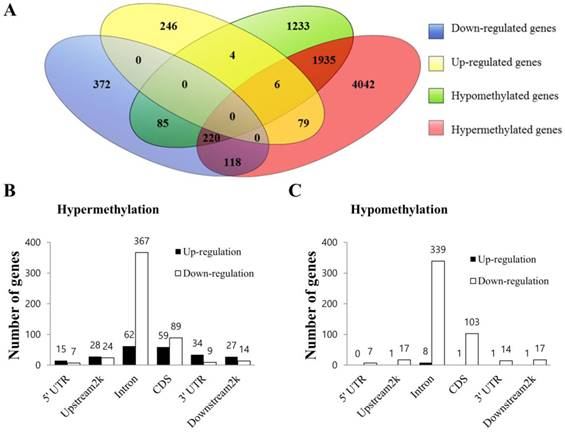
\includegraphics[width=0.8\textwidth]{journal-of-cancer_sample-result}}
%	\caption{یک نمونه نمودار خلاصه برای نمایش نوآوری در نتایج
%		%\cite{kim2016integrated}
%	}
%	\label{fig:sampleDiagram}
%\end{figure}\\
%طبیعتاً به صلاحدید نگارنده، شکل‌ها و نمودار‌ها می توانند در بخش های مختلف، خصوصا فصل
%\ref{chap:results}
%مورد استفاده قرار گیرند.
%
%\subsection{تعریف واژه‌ها (اختیاری)}
%در این قسمت محقق باید واژه‌هایی را که ممکن است برای خواننده آشنا نباشد، تعریف کند.
%
%\subsection{خلاصه فصل‌ها}
%در آخرین قسمتِ فصل اول پایان‌نامه، خلاصه‌ای اشاره‌وار از فصل‌های آتی آورده می‌شود تا خواننده بتواند تصویری واضح از دیگر قسمت‌های پایان‌نامه در ذهن خود ترسیم کند.
%
%\section{جمع‌بندی}
%در این فصل به دو مقولهٔ نحوه استفاده از قالب \پ دانشگاه تهران و نیز ویژگی‌هایی که محتویات فصل اول پایان‌نامه (یعنی مقدمه) باید داشته باشند، پرداخته شد. با توجه به اینکه این راهنما نحوه استفاده از قالب را شرح داده، ملزومات محتوایی هر فصل پایان‌نامه را توضیح می‌دهد و در پیوست‌ها نیز نحوهٔ کار با لاتک را یادآوری خواهد کرد، بنابراین مطالعهٔ کامل آن مقداری وقت شما را خواهد گرفت؛ اما مطمئن باشید از اتلاف وقت شما در ادامه کارتان تا حد زیادی جلوگیری خواهد کرد. در نوشتن متن حاضر سعی شده است علاوه بر ایجاد یک قالب لاتک برای پایان‌نامه‌های دانشگاه تهران، نکات محتوایی هر فصل نیز گوشزد گردد. طبیعتاً برای نگارش پایان‌نامهٔ خود می‌بایست مطالب تمام فصل‌ها را خودتان بازنویسی کنید.
%
%در ادامهٔ این راهنما، تنها فصل‌هایی که یک پایان‌نامه باید داشته باشد و نیز خصوصیات یا ساختاری که محتویات هر فصل باید از آنها برخوردار باشد%
%\footnote{از روی فایل «تمپلیت نگارش و تدوین پایان‌نامه \cite{UTThesisGuide}»}،
%آورده می‌شوند. نهایتاً  در پیوست‌ها، مطالبی در باب یادآوری دستورات لاتک، نحوه نوشتن فرمول‌ها، تعاریف، قضایا، مثال‌ها، درج تصاویر، نمودارها، جداول و الگوریتم‌ها و نیز مدیریت مراجع، آمده است.
%
%همچنین توصیه اکید دارم که رفع خطاهایی که احتمالاً با آنها مواجه می‌شوید را به آخر موکول نفرمایید و به محض برخورد با خطا، آن را اشکال‌زدایی و برطرف نمائید.!
%و
%\verb!% !TeX root=../main.tex
\chapter{پیشینه پژوهش}
%\thispagestyle{empty} 
\section{تولید آزمایه به صورت خودکار}
تولید خودکار آزمایه 
\LTRfootnote{Testcase}
به معنای ایجاد سناریوهای آزمون به صورت خودکار، بدون نیاز به دخالت دستی است. در این روش آزمونگر از تکنیک‌ها و ابزارهای ویژه‌ای استفاده می‌کند تا سناریوهای متنوعی برای آزمون نرم‌افزار تحت آزمون
\LTRfootnote{System Under Test}
 ایجاد کند. مزایای این روش عبارت‌اند از:
\begin{itemize}
	\item \textbf{پوشش گسترده‌تر آزمون:} تولید خودکار آزمایه‌ها، مواردی را پوشش می‌دهد که ممکن است در آزمون‌های دستی نادیده گرفته شوند. این امر به ویژه در آزمون نرم‌افزارهای پیچیده و بزرگ اهمیت بیشتری دارد.
	\item \textbf{افزایش کارایی آزمون:} با خودکارسازی فرآیند تولید آزمایه‌ها، می‌توان تعداد زیادی آزمایه در مدت زمان کوتاهی ایجاد کرد، که این کارایی در فازهای توسعه و نگهداری نرم‌افزار بسیار مفید است.
	\item \textbf{کشف باگ‌های ناشناخته:} تولید خودکار آزمایه‌ها به شناسایی باگ‌هایی کمک می‌کند که ممکن است در سناریوهای پیش‌بینی‌نشده رخ دهند. آزمون‌های تصادفی به خصوص در این زمینه بسیار مؤثر هستند.
	\item \textbf{کاهش دخالت انسانی:} خودکارسازی تولید آزمایه‌ها باعث کاهش خطاهای انسانی می‌شود و دقت و اطمینان آزمون‌ها را افزایش می‌دهد.
\end{itemize}

\section{آزمون تصادفی}
آزمون تصادفی \LTRfootnote{Random Testing} یک روش آزمون نرم‌افزار جعبه سیاه\LTRfootnote{Black Box Testing} است که در آن سیستم تحت آزمون با ورودی‌های تولید شده به صورت تصادفی ارزیابی می‌شود. هدف اصلی آزمون تصادفی، شناسایی اشکالات نرم‌افزار و اطمینان از قابلیت اطمینان و استحکام نرم‌افزار در مواجهه با انواع مختلف سناریوهای ورودی است.
\subsection{فرآیند تولید آزمایه توسط آزمون تصادفی}
فرآیند تولید آزمایه به صورت خودکار توسط روش آزمون تصادفی را می‌توان به صورت زیر ترسیم کرد:

\begin{enumerate}
	\item \textbf{تعریف فضای ورودی\LTRfootnote{Input Domain}:} در این مرحله محدوده و نوع ورودی‌هایی که نرم‌افزار می‌تواند بپذیرد، مشخص می‌گردد. این شامل تعیین دامنه‌های ورودی و محدودیت‌ها برای اطمینان از صحت موارد آزمون تولید شده است.
	\item \textbf{تولید موارد آزمون:} مجموعه‌ای از مقادیر ورودی به صورت تصادفی در داخل فضای ورودی تعریف شده تولید می‌شود. این ورودی‌ها باید طیف گسترده‌ای از سناریوهای ممکن را پوشش دهند تا احتمال کشف اشکالات افزایش یابد.
	\item \textbf{اجرای آزمون:} نرم‌افزار با استفاده از ورودی‌های تولید شده تصادفی اجرا شده و رفتار و خروجی‌های آن برای هر گونه ناهنجاری یا نتایج غیرمنتظره نظارت می‌شود.
	\item \textbf{ارزیابی خروجی‌ها:} خروجی‌های واقعی نرم‌افزار با خروجی‌های مورد انتظار (در صورت موجود بودن) مقایسه می‌شوند تا هر گونه تفاوت شناسایی گردد. در مواردی که خروجی مورد انتظار از پیش تعیین نشده است، از روش‌های اکتشافی یا اوراکل‌ها
		\LTRfootnote{Oracle}
	 برای ارزیابی درستی رفتار سیستم تحت آزمون استفاده می‌شود.
	\item \textbf{شناسایی و تحلیل اشکالات:} هر گونه انحراف یا خرابی که در حین آزمون شناسایی شود، تحلیل می‌گردد تا علل زیربنایی آن تشخیص داده شود.
\end{enumerate}


\subsection{مزایای آزمون تصادفی}
آزمون تصادفی چندین مزیت دارد که آن را به یک تکنیک ارزشمند در آزمون نرم‌افزار تبدیل می‌کند:
\begin{itemize}
	\item \textbf{سادگی:} این روش به سادگی قابل پیاده‌سازی است و نیازی به دانش عمیق از ساختار داخلی نرم‌افزار ندارد. موارد آزمون می‌توانند به صورت خودکار و بدون تلاش دستی، به صورت نامحدود تولید شوند.
	\item \textbf{خودکارسازی:} آزمون تصادفی می‌تواند به طور کامل خودکار شود و امکان آزمون پیوسته و بدون نیاز به نظارت انسانی را فراهم کند. این امر نیاز به دخالت انسانی را کاهش می‌دهد.
	\item \textbf{پوشش گسترده:} با تولید مجموعه‌ای متنوع از ورودی‌های تصادفی، آزمون تصادفی می‌تواند طیف گسترده‌ای از سناریوهای ورودی را پوشش دهد. این امر احتمال کشف اشکالات نادر یا غیرمنتظره‌ای که ممکن است از طریق دیگر روش‌های آزمون نرم‌افزار شناسایی نشوند را افزایش می‌دهد.
\end{itemize}

\subsection{معایب آزمون تصادفی}
با وجود مزایای آن، آزمون تصادفی چندین محدودیت دارد که می‌تواند بر اثربخشی آن تأثیر بگذارد:
\begin{itemize}
	\item \textbf{ناکارآمدی:} این روش می‌تواند از نظر زمان و منابع محاسباتی ناکارآمد باشد. بسیاری از ورودی‌های تولید شده ممکن است موارد آزمون معناداری را تحریک نکنند، که منجر به هدر رفتن تلاش‌ها و منابع استفاده شده جهت آزمون می‌شود.
	\item \textbf{تکرارپذیری:} آزمون تصادفی ممکن است موارد آزمون تکراری تولید کند که ارزش افزوده زیادی ندارند. نبود تمرکز بر نواحی بحرانی می‌تواند منجر به حجم بالای آزمون‌ها با نرخ شناسایی اشکال پایین شود.
	\item \textbf{تمرکز محدود:} آزمون تصادفی نواحی ورودی خاص یا نقاط خرابی بحرانی را اولویت‌بندی نمی‌کند. بنابراین، ممکن است اشکالات مهمی که در نواحی کمتر آزمون شده متمرکز شده‌اند را نادیده بگیرد.
\end{itemize}

%===============================================================================================================

\section{آزمون تصادفی تطبیقی}
آزمون تصادفی تطبیقی \LTRfootnote{Adaptive Random Testing}  با هدف بهبود آزمون تصادفی سنتی به وجود آمد و به ناکارآمدی‌ها و محدودیت‌های آن پرداخت. مفهوم آزمون تصادفی تطبیقی برای افزایش قابلیت‌های شناسایی اشکال آزمون تصادفی، با استفاده از استراتژی‌های تطبیقی که انتخاب موارد آزمون را هدایت می‌کنند، معرفی شد. آزمون تصادفی تطبیقی هدف دارد تا نرخ شناسایی اشکال بهتر را با حفظ مزایای سادگی و خودکارسازی آزمون تصادفی، بیشتر کند.

\subsection{فرضیه اصلی آزمون تصادفی تطبیقی}

توسعه آزمون تصادفی تطبیقی به دلیل نیاز به کاهش تکرارپذیری و ناکارآمدی مرتبط با تولید موارد آزمون به صورت تصادفی خالص به وجود آمد. محققان مشاهده کردند که اشکالات نرم‌افزار تمایل دارند در برخی نواحی فضای ورودی متمرکز شوند و به عبارت دیگر \textbf{نقاط خطا و شکست درون دامنه ورودی به صورت ناحیه‌ای هستند و تمایل به پیوسته بودن دارند.} در نتیجه هر چه تراکم آزمایه‌ها روی دامنه ورودی بیشتر باشد، احتمال کشف خطای جدید بیشتر خواهد بود. آزمون تصادفی تطبیقی از این مشاهده بهره می‌برد و از بازخورد موارد آزمون قبلی برای هدایت تولید موارد آزمون بعدی استفاده می‌کند. به طور کلی، آزمون تصادفی تطبیقی، آزمون تصادفی سنتی را با استفاده از تکنیک‌هایی که توزیع یکنواخت‌تری از موارد آزمون را در سراسر فضای ورودی تضمین می‌کنند، تقویت می‌کند. اصل کلیدی روش آزمون تصادفی تطبیقی این است که حداکثر تنوع موارد آزمون را به دست آورد و به این ترتیب، احتمال شناسایی خطا را افزایش دهد.

\subsection{فرآیند تولید آزمایه توسط آزمون تصادفی تطبیقی}

فرآیند تولید آزمایه به صورت خودکار توسط روش آزمون تصادفی تطبیقی را می‌توان به صورت زیر ترسیم کرد:
\begin{itemize}
	\item \textbf{تولید مجموعه کاندید\LTRfootnote{Candidate Set}:} در این مرحله ابتدایی، یک مجموعه‌ای از آزمایه‌ها با استفاده از روش آزمون تصادفی تولید می‌شود. این آزمایه‌ها به صورت تصادفی روی فضای ورودی تعریف شده از نرم‌افزار ایجاد می‌شوند.
	\item \textbf{انتخاب آزمایه:} از مجموعه کاندید تولید شده، یک آزمایه بر اساس یک استراتژی خاص که منحصراً به روش آزمون تصادفی تطبیقی مربوط است، انتخاب می‌شود. این استراتژی معمولاً به منظور به حداکثر رساندن فاصله آزمایه‌ها در فضای ورودی عمل می‌کند. با انتخاب آزمایه‌هایی که به طور گسترده‌تری پراکنده شده‌اند، آزمون تصادفی تطبیقی سعی دارد که احتمال کشف خطاها را نسبت به آزمون تصادفی سنتی افزایش دهد.
	\item \textbf{تکرار:} آزمایه انتخاب شده به مجموعه آزمایه‌های انتخاب شده \LTRfootnote{Executed Set}اضافه می‌شود و مراحل فوق به صورت تکراری انجام می‌شود. فرآیند تولید یک مجموعه کاندید جدید و انتخاب یک آزمایه ادامه می‌یابد تا زمانی که شرط خاتمه ارضاء شود که برای مثال شرط خاتمه می‌تواند رسیدن به تعداد مشخصی آزمایه باشد.
\end{itemize}
با دنبال کردن این مراحل، آزمون تصادفی تطبیقی تلاش می‌کند تا با تمرکز بر توزیع یکنواخت‌تر آزمایه‌ها، قابلیت کشف خطا را در مقایسه با آزمون تصادفی سنتی بهبود بخشد.

\subsection{مزایای آزمون تصادفی تطبیقی}
آزمون تصادفی تطبیقی چندین مزیت دارد که آن را به جایگزینی برتر برای آزمون تصادفی سنتی تبدیل می‌کند. در ادامه به برخی از این مزیت‌ها اشاره شده است:
\begin{itemize}
	\item \textbf{کاهش تکرارپذیری:} آزمون تصادفی تطبیقی با تولید موارد آزمون متنوع تکرارپذیری را کاهش می‌دهد. این امر ارزش هر مورد آزمون را به حداکثر می‌رساند و تلاش‌های بیهوده آزمون را به حداقل می‌رساند.
	\item \textbf{افزایش کارایی و نرخ شناسایی اشکال بالاتر:}‌ به دنبال کاهش تکرارپذیری موارد آزمون، کارایی روش آزمون تصادفی تطبیقی افزایش می‌یابد و فرآیند آزمون را بهبود می‌بخشد، که این خود منجر به نرخ شناسایی اشکال بالاتر با تعداد آزمایه کمتر می‌شود.
	\item \textbf{پوشش متعادل:} روش آزمون تصادفی تطبیقی، پوشش متعادل‌تری از فضای ورودی را به دست می‌آورد و خطر نادیده گرفتن نواحی مهم را کاهش می‌دهد. این پوشش جامع، استحکام کلی نرم‌افزار را افزایش می‌دهد.
	\item \textbf{بهینه‌سازی منابع:} با بهبود کارایی تولید موارد آزمون، آزمون تصادفی تطبیقی از منابع محاسباتی و زمانی بهینه استفاده می‌کند. این امر آزمون تصادفی تطبیقی را به یک راه‌حل عملی و مقیاس‌پذیر برای آزمون نرم‌افزار در مقیاس بزرگ تبدیل می‌کند.
\end{itemize}

\subsection{سربار محاسباتی پیاده سازی آزمون تصادفی تطبیقی}
در مرحله انتخاب آزمایه از فرآیند پیاده‌سازی روش آزمون تصادفی تطبیقی، لازم است که فاصله بین هر آزمایه درون مجموعه کاندید و هر آزمایه درون مجموعه آزمایه‌های انتخاب‌شده در مراحل قبلی محاسبه شود. آزمایه‌ای که بیشترین فاصله را با مجموعه آزمایه‌های انتخاب‌شده دارد، انتخاب می‌شود. در این مرحله، تعداد محاسبات فاصله باید به اندازه‌ی (تعداد آزمایه‌های درون مجموعه کاندید × تعداد آزمایه‌های درون مجموعه آزمایه‌های انتخاب‌شده) انجام شود. با افزایش تعداد اعضای مجموعه آزمایه‌های انتخاب‌شده در هر بار تکرار فرآیند، سربار محاسباتی الگوریتم آزمون تصادفی تطبیقی افزایش می‌یابد. همچنین، تعداد اعضای درون مجموعه کاندید نیز تأثیر مستقیمی بر افزایش سربار محاسباتی الگوریتم دارد. در ادامه، استراتژی‌هایی که تاکنون برای کاهش اندازه مجموعه کاندید، کاهش تعداد آزمایه‌های درون مجموعه آزمایه‌های انتخاب‌شده در مراحل قبلی الگوریتم، و در نهایت کاهش تعداد محاسبات فاصله ارائه شده‌اند، شرح داده می‌شود.

\subsubsection{اندازه مجموعه کاندید ثابت}
اولین و پرکاربردترین استراتژی پیاده‌سازی الگوریتم آزمون تصادفی تطبیقی، استراتژی "انتخاب آزمایه از مجموعه کاندید با اندازه ثابت\LTRfootnote{Fixed Sized Candidate Set (FSCS)}" است. در این استراتژی، که توسط [نام پژوهشگر/منبع] ارائه شده است، اندازه مجموعه کاندید در کل روند اجرای الگوریتم ثابت در نظر گرفته می‌شود. بهترین مقدار برای اندازه مجموعه کاندید طبق پژوهش [نام پژوهشگر/منبع] برابر با ۱۰ اعلام شده است. البته، هر چه اندازه مجموعه کاندید را افزایش دهیم، این امر می‌تواند بر اثربخشی آزمایه‌های نهایی تأثیر داشته باشد. اما بر اساس این پژوهش، هنگامی که اندازه مجموعه کاندید از ۱۰ بیشتر باشد، میزان افزایش اثربخشی مجموعه آزمایه‌ها خیلی قابل توجه نیست.

\subsubsection{بزرگ شدن فضای آزمون در آزمون تصادفی تطبیقی}
یکی از چالش‌های اصلی و مهم در آزمون تصادفی تطبیقی، بزرگ شدن فضای آزمون است. با افزایش تعداد آزمایه‌های انتخاب شده، محاسبه فاصله هر آزمایه جدید با آزمایه‌های قبلی زمان‌بر و ناکارآمد می‌شود. این مسئله باعث افزایش پیچیدگی محاسباتی و کاهش کارایی فرآیند آزمون می‌شود. برای مقابله با این مشکل، استراتژی‌های مختلفی ارائه شده‌اند که هدف آن‌ها کاهش فضای آزمون و بهبود کارایی تولید آزمایه‌ها است.
\begin{itemize}
	\item \textbf{استراتژی فراموشی\LTRfootnote{Forgetting Strategy}:} استراتژی فراموشی به منظور مدیریت فضای آزمون و جلوگیری از بزرگ شدن بیش از حد آن استفاده می‌شود. در این روش، زمانی که مجموعه آزمایه‌های از قبل انتخاب‌شده به توزیع یکنواخت مناسبی می‌رسند، این مجموعه پاک می‌شود. با این کار، فقط آزمایه‌های جدیدتر و مرتبط‌تر در فرآیند محاسبه فاصله‌ها لحاظ می‌شوند. در این استراتژی با پاک کردن آزمایه‌های قدیمی‌تر، حجم داده‌های مورد نیاز برای محاسبه فاصله‌ها کاهش می‌یابد و محاسبات سریع‌تر و کارآمدتر انجام می‌شود. البته، احتمال از دست رفتن اطلاعات مفید از آزمایه‌های قبلی وجود دارد و همچنین معیارهای فراموشی باید به دقت تنظیم شوند تا بهترین نتیجه حاصل شود.
	
	\item \textbf{خوشه‌بندی \lr{K}-مرکز\LTRfootnote{K-means Clustering Strategy}:} خوشه‌بندی \lr{K}-مرکز یکی دیگر از استراتژی‌های کاهش فضای آزمون است. در این روش، آزمایه‌های انتخاب‌شده به خوشه‌هایی تقسیم می‌شوند و هر خوشه با یک نماینده (میانگین) که مرکز خوشه است، مشخص می‌شود. برای انتخاب آزمایه جدید، فاصله بین آزمایه‌های کاندید و نمایندگان خوشه‌ها محاسبه می‌شود. این استراتژی علاوه بر کاهش تعداد محاسبات فاصله، باعث مدیریت بهتر فضای آزمون می‌شود و فضای آزمون به صورت خوشه‌بندی‌شده نگهداری می‌شود. با این حال، این روش ممکن است پیچیدگی اجرای الگوریتم را افزایش دهد و تعیین تعداد خوشه‌ها (\lr{K}) باید به دقت انجام شود تا بهترین نتیجه حاصل شود.
	
	\item \textbf{استراتژی شبکه‌بندی\LTRfootnote{Grid Strategy}:} در این روش، فضای ورودی به سلول‌های کوچکتری تقسیم می‌شود. آزمایه‌های انتخاب‌شده در هر سلول ذخیره می‌شوند و برای انتخاب آزمایه جدید، فقط سلول‌های مجاور مورد بررسی قرار می‌گیرند. این استراتژی علاوه بر کاهش تعداد محاسبات فاصله، باعث مدیریت بهتر فضای آزمون می‌شود و فضای آزمون به صورت شبکه‌بندی‌شده نگهداری می‌شود. با این حال، این روش به پیاده‌سازی دقیق شبکه‌بندی نیاز دارد و اندازه سلول‌ها باید به دقت تنظیم شود تا بهترین نتیجه حاصل شود.

\end{itemize}

\subsection{اولین پیاده‌سازی روش آزمون تصادفی تطبیقی}
اولین پیاده‌سازی روش آزمون تصادفی تطبیقی روی برنامه‌هایی با ورودی عددی\LTRfootnote{Numerical Input Domain} انجام شد. در این پیاده‌سازی، هر آزمایه که مجموعه‌ای از ورودی‌های عددی بود، به صورت یک نقطه درون یک فضای چندبعدی (تعداد ابعاد برابر با تعداد ورودی‌ها) مدل‌سازی شد. در ادامه، این الگوریتم روی یک مثال ساده بررسی می‌شود.

فرض کنید که یک برنامه به نام \lr{Sum} دارید که دو عدد به عنوان ورودی دریافت کرده و حاصل جمع آن‌ها را برمی‌گرداند. در این الگوریتم، آزمایه‌های این برنامه روی یک فضای دوبعدی به صورت نقطه مدل خواهند شد (برای مثال، آزمایه با ورودی‌های ۱۰ و ۱۵ در فضای ورودی دوبعدی نقطه \lr{(10,15)} را تشکیل می‌دهد) و فاصله بین آن‌ها، همان فاصله اقلیدسی\LTRfootnote{Euclidean distance} بین دو نقطه در نظر گرفته می‌شود.

این روش با روش آزمون تصادفی سنتی روی چند برنامه مختلف با ورودی عددی پیاده‌سازی شد و نتایج نشان داد که این روش از روش آزمون تصادفی سنتی کارایی و عملکرد بهتری دارد.

اما مهم‌ترین مشکل این روش این بود که تنها روی برنامه‌هایی با ورودی عددی قابل پیاده‌سازی بود. با این حال، این مسئله باعث شد که زمینه پژوهشی جدیدی برای محققان ایجاد شود تا راهکاری برای محاسبه فاصله بین دو آزمایه با ورودی‌های غیرعددی\LTRfootnote{Obejctive} ارائه دهند. در اکثر راهکارهای ارائه‌شده، تلاش بر این بوده که هر آزمایه را به عنوان یک نقطه در یک یا چند فضای چندبعدی مدل کنند و سپس با استفاده از محاسبات ریاضی رایج برای محاسبه فاصله در فضاهای چندبعدی، مانند فاصله اقلیدسی، فاصله بین دو نقطه را به دست آورده و به عنوان فاصله بین دو آزمایه ارائه دهند.

\subsection{آخرین ایده پیاده‌سازی ارائه شده برای روش آزمون تصادفی تطبیقی}
آخرین روشی که تاکنون در این حوزه توسط [نام پژوهشگر/منبع] ارائه شده است، شامل روش‌های \lr{WTClustering-ART} و \lr{TFClustering-ART} می‌باشد. در ادامه به بررسی دقیق ساختار و نحوه کارکرد هر کدام از این روش‌ها پرداخته شده است.

\subsubsection{تبدیل فرکانس }
کاهوچی و همکارانش روش‌هایی بر مبنای تبدیل فرکانس\LTRfootnote{Frequency Transform}، که قبلاً برای تبدیل رشته‌ها در جستجوی تشابه رشته‌ها استفاده می‌شد، پیشنهاد کردند. این روش یک رشته با طول تعریف‌شده را با تعداد دفعات هر کاراکتر در رشته به یک بردار فرکانس\LTRfootnote{Frequency Vector} تبدیل می‌کند. تعریف دقیق بردار فرکانس در ادامه آورده شده است.

\begin{itemize}
	\item \textbf{بردار فرکانس:}
	فرض کنید که \(\Sigma = \{m_1, m_2, \dots, m_n\}\) لیست توابع در یک برنامه فرضی باشد و \(s\) ترتیب فراخوانی توابع توسط آزمایه \(t\) باشد. حال بردار فرکانس به صورت 
	\(f(s) = \{f_1, f_2, \dots, f_n\}\)
	 تعریف خواهد شد که \(f_i\) تعداد دفعاتی است که تابع \(m_i\) در ترتیب فراخوانی توابع (\(s\)) حضور دارد.
	
	برای مثال فرض کنید که \(\Sigma = \{a, b, c, d, e\}\) و \(s = abddc\) ترتیب فراخوانی توابع در حین اجرای آزمایه \(t\) باشد. در این وضعیت، تابع \(a\) یک بار، \(b\) یک بار، \(c\) صفر بار، \(d\) دو بار و \(e\) یک بار فراخوانی شده است. در نتیجه:
	\[
	f(s) = \{1, 1, 0, 2, 1\}
	\]
	
	حال با توجه به اینکه هر آزمایه به یک لیست عددی با طول \(n\) (یک نقطه در فضای \(n\) بعدی) تبدیل شده است، اکنون می‌توان به سادگی فاصله بین آزمایه‌ها را با استفاده از محاسبه فاصله بین نقطه‌های متناظر آزمایه‌ها به دست آورد.
	
\end{itemize}

\subsubsection{تبدیل موجک}
اگرچه تبدیل فرکانس می‌تواند به راحتی آزمایه‌های شیء‌گرا را به بردارهایی برای اندازه‌گیری عدم تشابه تبدیل کند، اما فقط بر فرکانس فراخوانی توابع تمرکز می‌کند و به ترتیب فراخوانی توابع اهمیتی نمی‌دهد. از آنجایی که ترتیب واقعی فراخوانی توابع معمولاً بر نتایج اجرا تأثیر می‌گذارد، عدم تشابه محاسبه‌شده رضایت‌بخش نیست.

برای مثال، فرض کنید \(\Sigma = \{a, b, c, d, e\}\) و \(s_1 = acbe\) ترتیب فراخوانی توابع در آزمایه \(t_1\) و \(s_2 = bcae\) ترتیب فراخوانی توابع در آزمایه \(t_2\) باشد. بعد از انجام تبدیل فرکانس، دو بردار فرکانس\\ \(f(s_1) = f(s_2) = \{1, 1, 1, 0, 1\}\) به دست خواهد آمد. فاصله بین آزمایه \(t_1\) و \(t_2\) با توجه به مقایسه بردارهای فرکانس این دو آزمایه صفر است، در حالی که ترتیب فراخوانی توابع در دو آزمایه کاملاً یکسان نیست.

از این رو، روش تبدیل موجک در این مقاله ارائه شد که علاوه بر تعداد فراخوانی هر تابع، به ترتیب فراخوانی توابع نیز تا حدی اهمیت می‌دهد. تبدیل موجک\LTRfootnote{Wavelet Transform} ابزاری ریاضی است که برای تجزیه و تحلیل سیگنال‌ها و داده‌ها در حوزه زمان و فرکانس استفاده می‌شود. در این مقاله، از تبدیل موجک برای اندازه‌گیری عدم تشابه بین تست‌ کیس‌های شیءگرا استفاده می‌شود. این معیار با تجزیه و تحلیل سیگنال‌های مربوط به ویژگی‌های آزمایه‌ها، میزان تفاوت بین آن‌ها را محاسبه می‌کند. در روش
 \lr{ART\_WTClustering} 
 از موجک هار \LTRfootnote{Haar Wavelet} برای مدل‌سازی اطلاعات فرکانس و اطلاعات ترتیب فراخوانی توابع استفاده شده است. در ادامه، معیار تبدیل موجک با مثال توضیح داده شده است.

\begin{itemize}
	\item \textbf{تعریف تبدیل موجک آزمایه:}
فرض کنید \(s = m_1 m_2 \dots m_j\) ترتیب فراخوانی توابع باشد. \(s_1\) یک زیررشته از \(s\) است که حاوی نیمه اول عناصر \(s\) است و \(s_2\) یک زیررشته دیگر از \(s\) است که حاوی نیمه دوم عناصر \(s\) است. تبدیل موجک \(s\) به صورت \(W(s) = [A, B]\) تعریف می‌شود که \(A = f(s)\) و \(B = B_1 - B_2\) که \(B_1 = f(s_1)\) و \(B_2 = f(s_2)\) است.

برای مثال فرض کنید که \(\Sigma = \{a, b, c, d, e\}\) و \(s = abdde\) ترتیب فراخوانی توابع در حین اجرای آزمایه \(t\) باشد. حال مقادیر \(A\) , \(B\) و \(W(s)\) به صورت زیر محاسبه خواهند شد:
\begin{align*}
	A = f(s) &= \{1, 1, 0, 2, 1\} \\
	s_1 = ab \quad & \Rightarrow \quad B_1 = \{1, 1, 0, 0, 0\} \\
	s_2 = dde \quad &\Rightarrow \quad B_2 = \{0, 0, 0, 2, 1\} \\
	B = B_1 - B_2 \quad &\Rightarrow \quad B = \{1, 1, 0, -2, -1\} \\
	W(s) = [A, B] \quad &\Rightarrow \quad W(s) = \left[\{1, 1, 0, 2, 1\}, \{1, 1, 0, -2, -1\}\right]
\end{align*}

\item \textbf{محاسبه فاصله بین آزمایه‌‌ها:}
فرض کنید \(\Sigma = \{m_1, m_2, \dots, m_n\}\) لیست توابع درون یک برنامه فرضی باشد. اگر \(s_1\) ترتیب فراخوانی توابع توسط آزمایه \(t_1\) و \(s_2\) ترتیب فراخوانی توابع توسط آزمایه \(t_2\) باشد، آنگاه \(W(s_1) = [A_1, B_1]\) و \(W(s_2) = [A_2, B_2]\) خواهد بود که \(A_1 = \{A_{11}, A_{12}, \dots, A_{1n}\}\) و \(B_1 = \{B_{11}, B_{12}, \dots, B_{1n}\}\) و \(A_2 = \{A_{21}, A_{22}, \dots, A_{2n}\}\) و \(B_2 = \{B_{21}, B_{22}, \dots, B_{2n}\}\) که فاصله \(WT\_D\) بین این دو آزمایه به صورت زیر محاسبه خواهد شد:
\[
WT\_D(t_1, t_2) = \sqrt{\sum_{i=1}^{n} (A_{1i} - A_{2i})^2} + \sqrt{\sum_{i=1}^{n} (B_{1i} - B_{2i})^2}
\]


\end{itemize}

\subsubsection{تبدیل فرکانس سه‌بخشی}
تا حدی، استفاده مستقیم از تبدیل موجک برای آزمایه‌های شیءگرا نامناسب است. دلیل اصلی این است که، اگرچه دنباله فراخوانی توابع را به دو قسمت تقسیم می‌کند و آنها را حفظ می‌کند، اما تنها تفریق نیمه اول و دوم این دنباله نمی‌تواند تفاوت بین توالی فراخوانی توابع را نمایش دهد. برای پرداختن به این موضوع، در این مقاله پیشنهاد شده است که از تبدیل فرکانس سه‌بخشی \LTRfootnote{Trisection Frequency Conversion (TFC)} استفاده شود. این معیار نه تنها به تعداد فراخوانی هر تابع در حین اجرای آزمایه‌ها توجه دارد بلکه ترتیب فراخوانی توابع در حین اجرای آزمایه‌های مختلف نیز اهمیت دارد.

\begin{itemize}

\item \textbf{تعریف معیار تبدیل فرکانس سه‌بخشی:}
فرض کنید که \(s = m_1 m_2 \dots m_j\) ترتیب فراخوانی توابع در حین اجرای آزمایه \(t\) باشد و \(s_1\) نیمه اول \(s\) و \(s_2\) نیمه دوم \(s\) باشد. معیار تبدیل فرکانس سه‌بخشی برای \(s\) به صورت \(TF(s) = [A, B, C]\) نمایش داده می‌شود که \(A = f(s)\)، \(B = f(s_1)\) و \(C = f(s_2)\) است.

\item \textbf{محاسبه فاصله بین آزمایه‌‌ها:}

فرض کنید \(\Sigma = \{m_1, m_2, \dots, m_n\}\) لیست توابع در یک برنامه فرضی باشد. یک آزمایه \(t_1\) با دنباله فراخوانی توابع \(s_1\) و یک آزمایه \(t_2\) با دنباله فراخوانی توابع \(s_2\) را در نظر بگیرید. فرض کنید\\ \(TF(s_1) = [A_1, B_1, C_1]\) و \(TF(s_2) = [A_2, B_2, C_2]\) که در آن \(A_1 = \{A_{11}, A_{12}, \dots, A_{1n}\}\)، \(B_1 = \{B_{11}, B_{12}, \dots, B_{1n}\}\)، \(C_1 = \{C_{11}, C_{12}, \dots, C_{1n}\}\)، \(A_2 = \{A_{21}, A_{22}, \dots, A_{2n}\}\)، \(B_2 = \{B_{21}, B_{22}, \dots, B_{2n}\}\)، و \(C_2 = \{C_{21}, C_{22}, \dots, C_{2n}\}\). تفاوت ترتیب بین \(s_1\) و \(s_2\) به صورت \(\sum_{i=1}^{j} \left(1 - \delta_{s_{1i} s_{2i}}\right)\) تعریف می‌شود، که \(\delta_{s_{1i} s_{2i}}\) نماد دلتای کرونکر استاندارد است، به طوری که اگر \(s_{1i} = s_{2i}\) باشد آنگاه \(\delta_{s_{1i} s_{2i}} = 1\) و در غیر اینصورت \(\delta_{s_{1i} s_{2i}} = 0\). فاصله \(TFC\)  یا \(TFC\_D\) بین این دو آزمایه به صورت زیر تعریف می‌شود:

\[
TFC\_D(t_1, t_2) = \sqrt{\sum_{i=1}^{n} (A_{1i} - A_{2i})^2} + \sqrt{\sum_{i=1}^{n} (B_{1i} - B_{2i})^2}
\]
\[
+ \sqrt{\sum_{i=1}^{n} (C_{1i} - C_{2i})^2} + \sum_{i=1}^{n} \left(1 - \delta_{s_{1i} s_{2i}}\right)
\quad
\]

\end{itemize}

\subsubsection{مقایسه بین \(TFC\_D\) و \(WT\_D\):}
در اینجا به بررسی تفاوت‌های \(WT\_D\) و \(TFC\_D\) در یک مثال پرداخته شده است. دو آزمایه \(t_1\) و \(t_2\) را در نظر بگیرید که ترتیب فراخوانی توابع توسط این دو آزمایه به صورت \(s_1 = abce\) و \(s_2 = abec\) است که \(s_{11} = ab\)، \(s_{12} = ce\)، \(s_{21} = ab\) و \(s_{22} = ec\) است. در نتیجه:

\begin{align*}
	W(s_1) &= \left[\langle 1, 1, 1, 0, 1 \rangle, \langle 1, 1, -1, 0, -1 \rangle \right] \\
	W(s_2) &= \left[\langle 1, 1, 1, 0, 1 \rangle, \langle 1, 1, -1, 0, -1 \rangle \right]
\end{align*}

است و در نتیجه \({WT\_D}(s_1, s_2)\) برابر است با:

\[
WT\_D(s_1, s_2) = \sqrt{0^2 + 0^2 + 0^2 + 0^2 + 0^2} + \sqrt{0^2 + 0^2 + 0^2 + 0^2 + 0^2} = 0
\]
\textbf{}
از طرفی با توجه به تعریف \(TF(s_i)\) مقادیر \(TF(s_1)\) و \(TF(s_2)\) و \(TFC\_D(s_1, s_2)\) به صورت زیر محاسبه می‌شوند:
\[
TF(s_1) = \left[\langle 1, 1, 1, 0, 1 \rangle, \langle 1, 1, 0, 0, 0 \rangle, \langle 0, 0, 1, 0, 1 \rangle\right]
\]
\[
TF(s_2) = \left[\langle 1, 1, 1, 0, 1 \rangle, \langle 1, 1, 0, 0, 0 \rangle, \langle 0, 0, 1, 0, 1 \rangle\right]
\]

\(TFC\_D(s_1, s_2)\) به صورت زیر محاسبه می‌شود:

\begin{align*}
	TFC\_D(s_1, s_2) &= \sqrt{0^2 + 0^2 + 0^2 + 0^2 + 0^2} + \sqrt{0^2 + 0^2 + 0^2 + 0^2 + 0^2} \\
	&\quad + \sqrt{0^2 + 0^2 + 0^2 + 0^2 + 0^2} + \sum_{i=1}^{j} \left(1 - \delta_{s_{1i}s_{2i}}\right)
\end{align*}

که

\[
\sum_{i=1}^{j} \left(1 - \delta_{s_{1i}s_{2i}}\right) = (1-1) + (1-1)  + (1-0)  + (1-0) = 2
\]

بنابراین:

\[
TFC\_D(s_1, s_2) = 0 + 0 + 0 + 2 = 2 
\]

همانطور که مشاهده کردید،‌ فاصله \(TFC\) در این مثال نسبت به فاصله \(ٌُWT\)  به ترتیب فراخوانی توابع توسط آزمایه‌ها اهمیت بیشتری می دهد.


\newpage

	\begin{tikzpicture}[node distance=2.5cm]
		
		\node (start) [startstop] {\rl{به صورت تصادفی اولین مورد آزمایشی شئ‌گرا را ایجاد کرده و اجرا کنید}};
		\node (decision) [decision, below of=start, yshift=-1cm] {\rl{شرط خاتمه}};
		\node (output) [startstop, right of=decision, xshift=4cm] {\rl{خروجی آزمایه‌های تولید شده}};
		\node (process1) [process, below of=decision, yshift=-1cm] {\rl{اضافه کردن این آزمایه به مجموعه آزمایه‌های انتخاب شده در مراحل قبلی الگوریتم}};
		\node (process2) [process, below of=process1, yshift=-1cm] {\rl{تولید ۱۰ آزمایه شئ‌گرا جدید به عنوان مجموعه کاندید}};
		
		\node (process3) [process, below of=process2, yshift=-1cm, xshift=0.5cm, text width=7cm] {\rl{خوشه‌بندی مجموعه آزمایه‌های از قبل انتخاب شده به \rl{K} خوشه}};
		\node (process4) [process, below of=process3, yshift=-0.5cm] {\rl{تعیین نماینده هر خوشه برای ارزیابی آزمایه‌های کاندید}};
		\node (process5) [process, below of=process4, yshift=-0.5cm] {Select the candidate which has the smallest distance with the subset};
		
		\draw [arrow] (start) -- (decision);
		\draw [arrow] (decision) -- node[anchor=east] {No} (process1);
		\draw [arrow] (decision) -- node[anchor=north] {Yes} (output);
		\draw [arrow] (process1) -- (process2);
		\draw [arrow] (process2) -- (process3);
		\draw [arrow] (process3) -- (process4);
		\draw [arrow] (process4) -- (process5);
%		\draw [arrow] (process5.east) -| ++(4,0) |- (decision.east);
		
		% Adding labels ①, ②, ③
%		\node[draw=none, fill=none] at ($(process2)!0.5!(process3)$) {\textcircled{1}};
%		\node[draw=none, fill=none] at ($(process3)!0.5!(process4)$) {\textcircled{2}};
%		\node[draw=none, fill=none] at ($(process4)!0.5!(process5)$) {\textcircled{3}};
		
	\end{tikzpicture}



\subsection{روش‌های مختلف انتخاب آزمایه بر اساس فاصله}


\subsection{نقطه اشتراک اکثر روش‌های پیاده‌سازی الگوریتم آزمون تصادفی تطبیقی}

\section{روش تقسیم‌بندی فضای ورودی}

\subsection{فرآیند تولید آزمایه توسط روش تقسیم‌بندی فضای ورودی}

%===============================================================================================================




%
%
%
%\newpage
%\section{مقدمه}
%هدف از این فصل که با عنوان‌های  «مروری بر ادبیات موضوع%
%\LTRfootnote{Literature Review}»،
%«مروری بر منابع» و یا «مروری بر پیشینه تحقیق%
%\LTRfootnote{Background Research}»
%معرفی می‌شود، بررسی و طبقه‌بندی یافته‌های تحقیقات دیگر محققان در سطح دنیا و تعیین و شناسایی خلأهای تحقیقاتی است. آنچه را که تحقیق شما به دانش موجود اضافه می‌کند، مشخص کنید. طرح پیشینه تحقیق%
%\LTRfootnote{Background Information}
%یک مرور محققانه است و تا آنجا باید پیش برود که پیش‌زمینهٔ تاریخی مناسبی از تحقیق را بیان کند و جایگاه تحقیق فعلی را در میان آثار پیشین نشان دهد. برای این منظور منابع مرتبط با تحقیق را بررسی کنید، البته نه آنچنان گسترده که کل پیشینه تاریخی بحث را در برگیرد. برای نوشتن این بخش:
%\begin{itemize}
%	\item
%	دانستنی‌های موجود و پیش‌زمینهٔ تاریخی و وضعیت کنونی موضوع را چنان بیان کنید که خواننده بدون مراجعه به منابع پیشین، نتایج حاصل از مطالعات قبلی را درک و ارزیابی کند.
%	\item
%	نشان دهید که بر موضوع احاطه دارید. پرسش تحقیق را همراه بحث و جدل‌ها و مسائل مطرح شده بیان کنید و مهم‌ترین تحقیق‌های انجام شده در این زمینه را معرفی نمائید.
%	\item
%	ابتدا مطالب عمومی‌تر و سپس پژوهش‌های مشابه با کار خود را معرفی کرده و نشان دهید که تحقیق شما از چه جنبه‌ای با کار دیگران تشابه یا تفاوت دارد.
%	\item
%	اگر کارهای قبلی را خلاصه کرده‌اید، از پرداختن به جزئیات غیرضروری بپرهیزید. در عوض، بر یافته‌ها و مسائل روش‌شناختی مرتبط و نتایج اصلی تأکید کنید و اگر بررسی‌ها و منابع مروری عمومی دربارهٔ موضوع موجود است، خواننده را به آنها ارجاع دهید.
%\end{itemize}
%
%\section{تعاریف، اصول و مبانی نظری}
%این قسمت ارائهٔ خلاصه‌ای از دانش کلاسیک موضوع است. این بخش الزامی نیست و بستگی به نظر استاد راهنما دارد.
%
%\section{مروری بر ادبیات موضوع}
%در این قسمت باید به کارهای مشابه دیگران در گذشته اشاره کرد و وزن بیشتر این قسمت بهتر است به مقالات ژورنالی سال‌های اخیر (۲ تا ۳ سال) تخصیص داده شود. به نتایج کارهای دیگران با ذکر دقیق مراجع باید اشاره شده و جایگاه و تفاوت تحقیق شما نیز با کارهای دیگران مشخص شود. استفاده از مقالات ژورنال‌های معتبر در دو یا سه سال اخیر، می‌تواند به اعتبار کار شما بیافزاید.
%
%\section{نتیجه‌گیری}
%‌در نتیجه‌گیری آخر این فصل، با توجه به بررسی انجام شده بر روی مراجع تحقیق، بخش‌های قابل گسترش و تحقیق در آن حیطه و چشم‌اندازهای تحقیق مورد بررسی قرار می‌گیرند.	در برخی از تحقیقات، نتیجه نهایی فصل روش تحقیق، ارائهٔ یک چارچوب کار تحقیقی 
%\lr{(research framework)}
است.!
%را در فایل 
%\lr{main.tex}،
%غیرفعال%
%\footnote{
%برای غیرفعال کردن یک دستور، کافی است در ابتدای آن، علامت درصد انگلیسی (\%) بگذارید.
%}
% کنید. در غیر این صورت، ابتدا مطالب دو فصل اول پردازش شده و سپس مطالب فصل ۳ پردازش می‌شود که این کار باعث طولانی شدن زمان پردازش می‌گردد. هر زمان که خروجی کل \پ را خواستید، تمام فصل‌ها را دوباره در
%\lr{main.tex}
%فعال نمائید.
%بدیهتاً لازم نیست فصل‌های \پ را به ترتیب تایپ کنید. مثلاً می‌توانید ابتدا مطالب فصل ۳ را تایپ نموده و سپس مطالب فصل ۱ را تایپ کنید. 
%\subsubsection{مراجع}
%برای وارد کردن مراجع \پ کافی است فایل 
%\lr{MyReferences.bib}
%را باز کرده و مراجع خود را به شکل اقلام نمونهٔ داخل آن، وارد کنید.  سپس از \lr{bibtex} برای تولید مراجع با قالب مناسب استفاده نمائید. برای توضیحات بیشتر بخش \ref{Sec:Ref} از پیوست \ref{app:latexIntro} و نیز پیوست \ref{app:refMan} را ببینید.
%
%\subsubsection{واژه‌نامه فارسی به انگلیسی و برعکس}
%برای وارد کردن معادل فارسی اصطلاحات لاتین در متن و تهیه فهرست واژه‌نامه از آنها، از بستهٔ
%\lr{glossaries}
%و نرم‌افزار
%\lr{xindy}
%استفاده می‌شود. بدین منظور کافی است اصطلاحات لاتین و ترجمهٔ آنها را در فایل
%\lr{words.tex}
%وارد کرده و هر جای متن که خواستید با دستورات
%\verb|gls{label}|
%یا \verb|glspl{label}|
%معادل فارسی مفرد یا جمع یک اصطلاح را بیاورید.
%
%مثلا در اینجا، واژهٔ
%«\gls{Action}»
%برای بار اول و دوباره
%«\gls{Action}»
%برای بار دوم در متن ظاهر شده است.
%جهت توضیحات بیشتر به پیوست
%\ref{app:refMan}
%مراجعه کنید.
%\subsubsection{نمایه}
%برای وارد کردن نمایه، باید از 
%\lr{xindy}
%استفاده کنید. 
%%زیرا 
%%\lr{MakeIndex}
%%با حروف «گ»، «چ»، «پ»، «ژ» و «ک» مشکل دارد و ترتیب الفبایی این حروف را رعایت نمی‌کند. همچنین، فاصله بین هر گروه از کلمات در 
%%\lr{MakeIndex}،
%%به درستی رعایت نمی‌شود که باعث زشت شدن حروف‌چینی این قسمت می‌شود. 
%راهنمای چگونگی کار با 
%\lr{xindy} 
%را می‌توانید در ویکی پارسی‌لاتک و یا مثالهای موجود در دی‌وی‌دی «مجموعه پارسی‌لاتک»، پیدا کنید.
%
%\subsection{اگر سوالی داشتم، از کی بپرسم؟}
%برای پرسیدن سوال‌های خود موقع حروف‌چینی با زی‌پرشین، می‌توانید به
%\href{http://qa.parsilatex.com}{سایت پرسش و پاسخ پارسی‌لاتک}%
%\LTRfootnote{http://qa.parsilatex.com}
%یا
%\href{http://forum.parsilatex.com}{بایگانی تالارگفتگوی قدیمی پارسی‌لاتک}%
%\LTRfootnote{http://forum.parsilatex.com}
%مراجعه کنید. شما هم می‌توانید روزی به سوال‌های دیگران در اینترنت جواب دهید.
%بستهٔ زی‌پرشین و بسیاری از بسته‌های مرتبط با آن مانند
%\lr{bidi} و
%\lr{Persian-bib}،
%مجموعه پارسی‌لاتک، مثالهای مختلف موجود در آن، قالب پایان‌نامه دانشگاههای مختلف و سایت پارسی‌لاتک همه به صورت داوطلبانه توسط افراد گروه پارسی‌لاتک و گروه
%\lr{Persian TeX}
%و بدون هیچ کمک مالی انجام شده‌اند. کار اصلی نوشتن و توسعه زی‌پرشین توسط آقای وفا خلیقی انجام شده است که این کار بزرگ را به انجام رساندند.
%اگر مایل به کمک به گروه پارسی‌لاتک هستید به سایت این گروه مراجعه فرمایید:
%\begin{center}
%	\url{http://www.parsilatex.com}
%\end{center}
%
%\section{محتویات فصل اول یک پایان‌نامه}
%فصل اول یک پایان‌نامه باید به مقدمه یا کلیات تحقیق بپردازد.
%هدف از فصل مقدمه%
%\LTRfootnote{Introduction}،
%شرح مختصر مسأله تحقیق، اهمیت و انگیزه محقق از پرداختن به آن موضوع، بهمراه اشاره‌ای کوتاه به روش و مراحل تحقیق است. مقدمه، اولین فصل از ساختار اصلی \پ بوده و زمینه اطلاعاتی لازم را برای خواننده فراهم می‌آورد. در طول مقدمه باید سعی شود موضوع تحقیق با زبانی روشن، ساده و بطور عمیق و هدفمند به خواننده معرفی شود. این فصل باید خواننده را مجذوب و اهمیت موضوع تحقیق را آشکار سازد. در مقدمه باید با ارائهٔ سوابق، شواهد تحقیقی و اطلاعات موجود (با ذکر منبع) با روشی منظم، منطقی و هدف‌دار، خواننده را جهت داد و به سوی راه حل مورد نظر هدایت کرد. مقدمه مناسب‌ترین جا برای ارائهٔ اختصارات و بعضی توضیحات کلی است، توضیحاتی که شاید نتوان در مباحث دیگر آنها را شرح داد.
%
%مقدمه، یکی از ارکان اساسی و اصلی پایان نامه است که مهمترین قسمت‌های آن عبارتند از: 
%
%\subsection{عنوان تحقیق} 
%باید شناختی دقیق و روشن از حوزهٔ موضوع تحقیق را عرضه دارد و خالی از هرگونه ابهام و پیچیدگی باشد.
%
%\subsection{مسأله تحقیق}
%وظیفه اصلی مقدمه بیان این مطلب به خواننده است که چرا انجام تحقیق را به عهده گرفته‌اید. اگر دلیل شما برای انجام این کار پاسخگویی به سؤال مورد علاقه‌تان است، با مشکل زیادی روبه‌رو نخواهید بود. یکی از بهترین روش‌ها برای نوشتن مقدمهٔ یک پایان‌نامه، طرح پرسش یا پرسش‌هایی مهم و اساسی است که کار تحقیقاتی شما از آغاز تا پایان قصد پاسخ دادن به آن را دارد. گاهی می‌توانید ابتدا اهمیت موضوع را بیان و سپس پرسش خود را در آن موضوع مطرح کنید.
%
%\subsection{تاریخچه‌ای از موضوع تحقیق}
%به طور کلی تشریح روندهای تحقیقاتی در محدودهٔ مورد مطالعه، مستلزم ارجاع به کارهای دیگران است. بعضی از نویسندگان برای کارهای دیگران هیچ اعتباری قائل نمی‌شوند و در مقابل، بعضی دیگر از نویسندگان در توصیف کارهای دیگران، بسیار زیاده‌روی می‌کنند. اکثر مواقع، ارجاع به مقالات دو سال قبل از کارتان، بهتر از نوشتن سطرهای مرجع است. در این قسمت باید به طور مختصر به نظرات و تحقیقات مربوط به موضوع و یا مسائل و مشکلات حل نشده در این حوزه و همچنین توجه و علاقه جامعه به این موضوع، اشاره شود.
%
%\subsection{تعریف موضوع تحقیق}
%در این قسمت محقق، موضوع مورد علاقه و یا نیاز احساس شدهٔ خود را در حوزه تحقیق بیان می‌دارد و عوامل موجود در موقعیت را تعریف و تعیین می‌کند.
%
%\subsection{هدف یا هدف‌های کلی و آرمانی تحقیق}
%این قسمت باید با جملات مثبت و کلی طرح شود و از طولانی شدن مطالب پرهیز شود.
%
%\subsection{روش انجام تحقیق}
%در این قسمت، پژوهشگر روش کاری خود را بیان می‌دارد و شیوه‌های گوناگونی را که در گردآوری مطالب خود بکار برده، ذکر می‌کند. همچنین اگر روش آماری خاصی را در تهیه و تدوین اطلاعات به کار برده است، آن شیوه را نیز اینجا بیان می‌کند.
%
%\subsection{نوآوری، اهمیت و ارزش تحقیق}
%در این قسمت، در مورد نوآوری علمی و عملی تحقیق که محقق به آن دست خواهد یافت، بحث می‌شود. ممکن است لازم باشد تا برخی نمودارهای خلاصه در این بخش استفاده شوند. به عنوان مثال، نموداری از مقاله
%\cite{kim2016integrated}
%در شکل
%\ref{fig:sampleDiagram}
%آمده است.
%\begin{figure}[ht]
%	\centerline{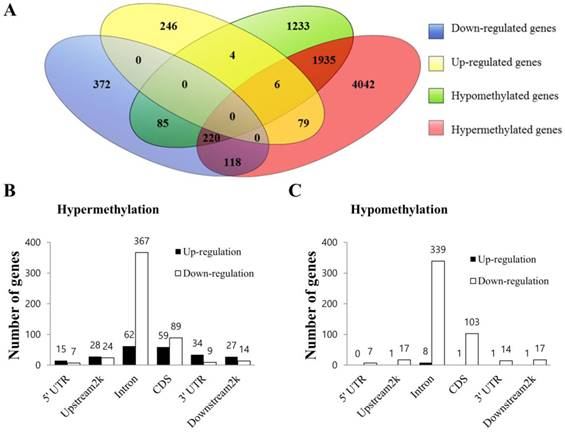
\includegraphics[width=0.8\textwidth]{journal-of-cancer_sample-result}}
%	\caption{یک نمونه نمودار خلاصه برای نمایش نوآوری در نتایج
%		%\cite{kim2016integrated}
%	}
%	\label{fig:sampleDiagram}
%\end{figure}\\
%طبیعتاً به صلاحدید نگارنده، شکل‌ها و نمودار‌ها می توانند در بخش های مختلف، خصوصا فصل
%\ref{chap:results}
%مورد استفاده قرار گیرند.
%
%\subsection{تعریف واژه‌ها (اختیاری)}
%در این قسمت محقق باید واژه‌هایی را که ممکن است برای خواننده آشنا نباشد، تعریف کند.
%
%\subsection{خلاصه فصل‌ها}
%در آخرین قسمتِ فصل اول پایان‌نامه، خلاصه‌ای اشاره‌وار از فصل‌های آتی آورده می‌شود تا خواننده بتواند تصویری واضح از دیگر قسمت‌های پایان‌نامه در ذهن خود ترسیم کند.
%
%\section{جمع‌بندی}
%در این فصل به دو مقولهٔ نحوه استفاده از قالب \پ دانشگاه تهران و نیز ویژگی‌هایی که محتویات فصل اول پایان‌نامه (یعنی مقدمه) باید داشته باشند، پرداخته شد. با توجه به اینکه این راهنما نحوه استفاده از قالب را شرح داده، ملزومات محتوایی هر فصل پایان‌نامه را توضیح می‌دهد و در پیوست‌ها نیز نحوهٔ کار با لاتک را یادآوری خواهد کرد، بنابراین مطالعهٔ کامل آن مقداری وقت شما را خواهد گرفت؛ اما مطمئن باشید از اتلاف وقت شما در ادامه کارتان تا حد زیادی جلوگیری خواهد کرد. در نوشتن متن حاضر سعی شده است علاوه بر ایجاد یک قالب لاتک برای پایان‌نامه‌های دانشگاه تهران، نکات محتوایی هر فصل نیز گوشزد گردد. طبیعتاً برای نگارش پایان‌نامهٔ خود می‌بایست مطالب تمام فصل‌ها را خودتان بازنویسی کنید.
%
%در ادامهٔ این راهنما، تنها فصل‌هایی که یک پایان‌نامه باید داشته باشد و نیز خصوصیات یا ساختاری که محتویات هر فصل باید از آنها برخوردار باشد%
%\footnote{از روی فایل «تمپلیت نگارش و تدوین پایان‌نامه \cite{UTThesisGuide}»}،
%آورده می‌شوند. نهایتاً  در پیوست‌ها، مطالبی در باب یادآوری دستورات لاتک، نحوه نوشتن فرمول‌ها، تعاریف، قضایا، مثال‌ها، درج تصاویر، نمودارها، جداول و الگوریتم‌ها و نیز مدیریت مراجع، آمده است.
%
%همچنین توصیه اکید دارم که رفع خطاهایی که احتمالاً با آنها مواجه می‌شوید را به آخر موکول نفرمایید و به محض برخورد با خطا، آن را اشکال‌زدایی و برطرف نمائید.!
%و
%\verb!% !TeX root=../main.tex
\chapter{پیشینه پژوهش}
%\thispagestyle{empty} 
\section{تولید آزمایه به صورت خودکار}
تولید خودکار آزمایه 
\LTRfootnote{Testcase}
به معنای ایجاد سناریوهای آزمون به صورت خودکار، بدون نیاز به دخالت دستی است. در این روش آزمونگر از تکنیک‌ها و ابزارهای ویژه‌ای استفاده می‌کند تا سناریوهای متنوعی برای آزمون نرم‌افزار تحت آزمون
\LTRfootnote{System Under Test}
 ایجاد کند. مزایای این روش عبارت‌اند از:
\begin{itemize}
	\item \textbf{پوشش گسترده‌تر آزمون:} تولید خودکار آزمایه‌ها، مواردی را پوشش می‌دهد که ممکن است در آزمون‌های دستی نادیده گرفته شوند. این امر به ویژه در آزمون نرم‌افزارهای پیچیده و بزرگ اهمیت بیشتری دارد.
	\item \textbf{افزایش کارایی آزمون:} با خودکارسازی فرآیند تولید آزمایه‌ها، می‌توان تعداد زیادی آزمایه در مدت زمان کوتاهی ایجاد کرد، که این کارایی در فازهای توسعه و نگهداری نرم‌افزار بسیار مفید است.
	\item \textbf{کشف باگ‌های ناشناخته:} تولید خودکار آزمایه‌ها به شناسایی باگ‌هایی کمک می‌کند که ممکن است در سناریوهای پیش‌بینی‌نشده رخ دهند. آزمون‌های تصادفی به خصوص در این زمینه بسیار مؤثر هستند.
	\item \textbf{کاهش دخالت انسانی:} خودکارسازی تولید آزمایه‌ها باعث کاهش خطاهای انسانی می‌شود و دقت و اطمینان آزمون‌ها را افزایش می‌دهد.
\end{itemize}

\section{آزمون تصادفی}
آزمون تصادفی \LTRfootnote{Random Testing} یک روش آزمون نرم‌افزار جعبه سیاه\LTRfootnote{Black Box Testing} است که در آن سیستم تحت آزمون با ورودی‌های تولید شده به صورت تصادفی ارزیابی می‌شود. هدف اصلی آزمون تصادفی، شناسایی اشکالات نرم‌افزار و اطمینان از قابلیت اطمینان و استحکام نرم‌افزار در مواجهه با انواع مختلف سناریوهای ورودی است.
\subsection{فرآیند تولید آزمایه توسط آزمون تصادفی}
فرآیند تولید آزمایه به صورت خودکار توسط روش آزمون تصادفی را می‌توان به صورت زیر ترسیم کرد:

\begin{enumerate}
	\item \textbf{تعریف فضای ورودی\LTRfootnote{Input Domain}:} در این مرحله محدوده و نوع ورودی‌هایی که نرم‌افزار می‌تواند بپذیرد، مشخص می‌گردد. این شامل تعیین دامنه‌های ورودی و محدودیت‌ها برای اطمینان از صحت موارد آزمون تولید شده است.
	\item \textbf{تولید موارد آزمون:} مجموعه‌ای از مقادیر ورودی به صورت تصادفی در داخل فضای ورودی تعریف شده تولید می‌شود. این ورودی‌ها باید طیف گسترده‌ای از سناریوهای ممکن را پوشش دهند تا احتمال کشف اشکالات افزایش یابد.
	\item \textbf{اجرای آزمون:} نرم‌افزار با استفاده از ورودی‌های تولید شده تصادفی اجرا شده و رفتار و خروجی‌های آن برای هر گونه ناهنجاری یا نتایج غیرمنتظره نظارت می‌شود.
	\item \textbf{ارزیابی خروجی‌ها:} خروجی‌های واقعی نرم‌افزار با خروجی‌های مورد انتظار (در صورت موجود بودن) مقایسه می‌شوند تا هر گونه تفاوت شناسایی گردد. در مواردی که خروجی مورد انتظار از پیش تعیین نشده است، از روش‌های اکتشافی یا اوراکل‌ها
		\LTRfootnote{Oracle}
	 برای ارزیابی درستی رفتار سیستم تحت آزمون استفاده می‌شود.
	\item \textbf{شناسایی و تحلیل اشکالات:} هر گونه انحراف یا خرابی که در حین آزمون شناسایی شود، تحلیل می‌گردد تا علل زیربنایی آن تشخیص داده شود.
\end{enumerate}


\subsection{مزایای آزمون تصادفی}
آزمون تصادفی چندین مزیت دارد که آن را به یک تکنیک ارزشمند در آزمون نرم‌افزار تبدیل می‌کند:
\begin{itemize}
	\item \textbf{سادگی:} این روش به سادگی قابل پیاده‌سازی است و نیازی به دانش عمیق از ساختار داخلی نرم‌افزار ندارد. موارد آزمون می‌توانند به صورت خودکار و بدون تلاش دستی، به صورت نامحدود تولید شوند.
	\item \textbf{خودکارسازی:} آزمون تصادفی می‌تواند به طور کامل خودکار شود و امکان آزمون پیوسته و بدون نیاز به نظارت انسانی را فراهم کند. این امر نیاز به دخالت انسانی را کاهش می‌دهد.
	\item \textbf{پوشش گسترده:} با تولید مجموعه‌ای متنوع از ورودی‌های تصادفی، آزمون تصادفی می‌تواند طیف گسترده‌ای از سناریوهای ورودی را پوشش دهد. این امر احتمال کشف اشکالات نادر یا غیرمنتظره‌ای که ممکن است از طریق دیگر روش‌های آزمون نرم‌افزار شناسایی نشوند را افزایش می‌دهد.
\end{itemize}

\subsection{معایب آزمون تصادفی}
با وجود مزایای آن، آزمون تصادفی چندین محدودیت دارد که می‌تواند بر اثربخشی آن تأثیر بگذارد:
\begin{itemize}
	\item \textbf{ناکارآمدی:} این روش می‌تواند از نظر زمان و منابع محاسباتی ناکارآمد باشد. بسیاری از ورودی‌های تولید شده ممکن است موارد آزمون معناداری را تحریک نکنند، که منجر به هدر رفتن تلاش‌ها و منابع استفاده شده جهت آزمون می‌شود.
	\item \textbf{تکرارپذیری:} آزمون تصادفی ممکن است موارد آزمون تکراری تولید کند که ارزش افزوده زیادی ندارند. نبود تمرکز بر نواحی بحرانی می‌تواند منجر به حجم بالای آزمون‌ها با نرخ شناسایی اشکال پایین شود.
	\item \textbf{تمرکز محدود:} آزمون تصادفی نواحی ورودی خاص یا نقاط خرابی بحرانی را اولویت‌بندی نمی‌کند. بنابراین، ممکن است اشکالات مهمی که در نواحی کمتر آزمون شده متمرکز شده‌اند را نادیده بگیرد.
\end{itemize}

%===============================================================================================================

\section{آزمون تصادفی تطبیقی}
آزمون تصادفی تطبیقی \LTRfootnote{Adaptive Random Testing}  با هدف بهبود آزمون تصادفی سنتی به وجود آمد و به ناکارآمدی‌ها و محدودیت‌های آن پرداخت. مفهوم آزمون تصادفی تطبیقی برای افزایش قابلیت‌های شناسایی اشکال آزمون تصادفی، با استفاده از استراتژی‌های تطبیقی که انتخاب موارد آزمون را هدایت می‌کنند، معرفی شد. آزمون تصادفی تطبیقی هدف دارد تا نرخ شناسایی اشکال بهتر را با حفظ مزایای سادگی و خودکارسازی آزمون تصادفی، بیشتر کند.

\subsection{فرضیه اصلی آزمون تصادفی تطبیقی}

توسعه آزمون تصادفی تطبیقی به دلیل نیاز به کاهش تکرارپذیری و ناکارآمدی مرتبط با تولید موارد آزمون به صورت تصادفی خالص به وجود آمد. محققان مشاهده کردند که اشکالات نرم‌افزار تمایل دارند در برخی نواحی فضای ورودی متمرکز شوند و به عبارت دیگر \textbf{نقاط خطا و شکست درون دامنه ورودی به صورت ناحیه‌ای هستند و تمایل به پیوسته بودن دارند.} در نتیجه هر چه تراکم آزمایه‌ها روی دامنه ورودی بیشتر باشد، احتمال کشف خطای جدید بیشتر خواهد بود. آزمون تصادفی تطبیقی از این مشاهده بهره می‌برد و از بازخورد موارد آزمون قبلی برای هدایت تولید موارد آزمون بعدی استفاده می‌کند. به طور کلی، آزمون تصادفی تطبیقی، آزمون تصادفی سنتی را با استفاده از تکنیک‌هایی که توزیع یکنواخت‌تری از موارد آزمون را در سراسر فضای ورودی تضمین می‌کنند، تقویت می‌کند. اصل کلیدی روش آزمون تصادفی تطبیقی این است که حداکثر تنوع موارد آزمون را به دست آورد و به این ترتیب، احتمال شناسایی خطا را افزایش دهد.

\subsection{فرآیند تولید آزمایه توسط آزمون تصادفی تطبیقی}

فرآیند تولید آزمایه به صورت خودکار توسط روش آزمون تصادفی تطبیقی را می‌توان به صورت زیر ترسیم کرد:
\begin{itemize}
	\item \textbf{تولید مجموعه کاندید\LTRfootnote{Candidate Set}:} در این مرحله ابتدایی، یک مجموعه‌ای از آزمایه‌ها با استفاده از روش آزمون تصادفی تولید می‌شود. این آزمایه‌ها به صورت تصادفی روی فضای ورودی تعریف شده از نرم‌افزار ایجاد می‌شوند.
	\item \textbf{انتخاب آزمایه:} از مجموعه کاندید تولید شده، یک آزمایه بر اساس یک استراتژی خاص که منحصراً به روش آزمون تصادفی تطبیقی مربوط است، انتخاب می‌شود. این استراتژی معمولاً به منظور به حداکثر رساندن فاصله آزمایه‌ها در فضای ورودی عمل می‌کند. با انتخاب آزمایه‌هایی که به طور گسترده‌تری پراکنده شده‌اند، آزمون تصادفی تطبیقی سعی دارد که احتمال کشف خطاها را نسبت به آزمون تصادفی سنتی افزایش دهد.
	\item \textbf{تکرار:} آزمایه انتخاب شده به مجموعه آزمایه‌های انتخاب شده \LTRfootnote{Executed Set}اضافه می‌شود و مراحل فوق به صورت تکراری انجام می‌شود. فرآیند تولید یک مجموعه کاندید جدید و انتخاب یک آزمایه ادامه می‌یابد تا زمانی که شرط خاتمه ارضاء شود که برای مثال شرط خاتمه می‌تواند رسیدن به تعداد مشخصی آزمایه باشد.
\end{itemize}
با دنبال کردن این مراحل، آزمون تصادفی تطبیقی تلاش می‌کند تا با تمرکز بر توزیع یکنواخت‌تر آزمایه‌ها، قابلیت کشف خطا را در مقایسه با آزمون تصادفی سنتی بهبود بخشد.

\subsection{مزایای آزمون تصادفی تطبیقی}
آزمون تصادفی تطبیقی چندین مزیت دارد که آن را به جایگزینی برتر برای آزمون تصادفی سنتی تبدیل می‌کند. در ادامه به برخی از این مزیت‌ها اشاره شده است:
\begin{itemize}
	\item \textbf{کاهش تکرارپذیری:} آزمون تصادفی تطبیقی با تولید موارد آزمون متنوع تکرارپذیری را کاهش می‌دهد. این امر ارزش هر مورد آزمون را به حداکثر می‌رساند و تلاش‌های بیهوده آزمون را به حداقل می‌رساند.
	\item \textbf{افزایش کارایی و نرخ شناسایی اشکال بالاتر:}‌ به دنبال کاهش تکرارپذیری موارد آزمون، کارایی روش آزمون تصادفی تطبیقی افزایش می‌یابد و فرآیند آزمون را بهبود می‌بخشد، که این خود منجر به نرخ شناسایی اشکال بالاتر با تعداد آزمایه کمتر می‌شود.
	\item \textbf{پوشش متعادل:} روش آزمون تصادفی تطبیقی، پوشش متعادل‌تری از فضای ورودی را به دست می‌آورد و خطر نادیده گرفتن نواحی مهم را کاهش می‌دهد. این پوشش جامع، استحکام کلی نرم‌افزار را افزایش می‌دهد.
	\item \textbf{بهینه‌سازی منابع:} با بهبود کارایی تولید موارد آزمون، آزمون تصادفی تطبیقی از منابع محاسباتی و زمانی بهینه استفاده می‌کند. این امر آزمون تصادفی تطبیقی را به یک راه‌حل عملی و مقیاس‌پذیر برای آزمون نرم‌افزار در مقیاس بزرگ تبدیل می‌کند.
\end{itemize}

\subsection{سربار محاسباتی پیاده سازی آزمون تصادفی تطبیقی}
در مرحله انتخاب آزمایه از فرآیند پیاده‌سازی روش آزمون تصادفی تطبیقی، لازم است که فاصله بین هر آزمایه درون مجموعه کاندید و هر آزمایه درون مجموعه آزمایه‌های انتخاب‌شده در مراحل قبلی محاسبه شود. آزمایه‌ای که بیشترین فاصله را با مجموعه آزمایه‌های انتخاب‌شده دارد، انتخاب می‌شود. در این مرحله، تعداد محاسبات فاصله باید به اندازه‌ی (تعداد آزمایه‌های درون مجموعه کاندید × تعداد آزمایه‌های درون مجموعه آزمایه‌های انتخاب‌شده) انجام شود. با افزایش تعداد اعضای مجموعه آزمایه‌های انتخاب‌شده در هر بار تکرار فرآیند، سربار محاسباتی الگوریتم آزمون تصادفی تطبیقی افزایش می‌یابد. همچنین، تعداد اعضای درون مجموعه کاندید نیز تأثیر مستقیمی بر افزایش سربار محاسباتی الگوریتم دارد. در ادامه، استراتژی‌هایی که تاکنون برای کاهش اندازه مجموعه کاندید، کاهش تعداد آزمایه‌های درون مجموعه آزمایه‌های انتخاب‌شده در مراحل قبلی الگوریتم، و در نهایت کاهش تعداد محاسبات فاصله ارائه شده‌اند، شرح داده می‌شود.

\subsubsection{اندازه مجموعه کاندید ثابت}
اولین و پرکاربردترین استراتژی پیاده‌سازی الگوریتم آزمون تصادفی تطبیقی، استراتژی "انتخاب آزمایه از مجموعه کاندید با اندازه ثابت\LTRfootnote{Fixed Sized Candidate Set (FSCS)}" است. در این استراتژی، که توسط [نام پژوهشگر/منبع] ارائه شده است، اندازه مجموعه کاندید در کل روند اجرای الگوریتم ثابت در نظر گرفته می‌شود. بهترین مقدار برای اندازه مجموعه کاندید طبق پژوهش [نام پژوهشگر/منبع] برابر با ۱۰ اعلام شده است. البته، هر چه اندازه مجموعه کاندید را افزایش دهیم، این امر می‌تواند بر اثربخشی آزمایه‌های نهایی تأثیر داشته باشد. اما بر اساس این پژوهش، هنگامی که اندازه مجموعه کاندید از ۱۰ بیشتر باشد، میزان افزایش اثربخشی مجموعه آزمایه‌ها خیلی قابل توجه نیست.

\subsubsection{بزرگ شدن فضای آزمون در آزمون تصادفی تطبیقی}
یکی از چالش‌های اصلی و مهم در آزمون تصادفی تطبیقی، بزرگ شدن فضای آزمون است. با افزایش تعداد آزمایه‌های انتخاب شده، محاسبه فاصله هر آزمایه جدید با آزمایه‌های قبلی زمان‌بر و ناکارآمد می‌شود. این مسئله باعث افزایش پیچیدگی محاسباتی و کاهش کارایی فرآیند آزمون می‌شود. برای مقابله با این مشکل، استراتژی‌های مختلفی ارائه شده‌اند که هدف آن‌ها کاهش فضای آزمون و بهبود کارایی تولید آزمایه‌ها است.
\begin{itemize}
	\item \textbf{استراتژی فراموشی\LTRfootnote{Forgetting Strategy}:} استراتژی فراموشی به منظور مدیریت فضای آزمون و جلوگیری از بزرگ شدن بیش از حد آن استفاده می‌شود. در این روش، زمانی که مجموعه آزمایه‌های از قبل انتخاب‌شده به توزیع یکنواخت مناسبی می‌رسند، این مجموعه پاک می‌شود. با این کار، فقط آزمایه‌های جدیدتر و مرتبط‌تر در فرآیند محاسبه فاصله‌ها لحاظ می‌شوند. در این استراتژی با پاک کردن آزمایه‌های قدیمی‌تر، حجم داده‌های مورد نیاز برای محاسبه فاصله‌ها کاهش می‌یابد و محاسبات سریع‌تر و کارآمدتر انجام می‌شود. البته، احتمال از دست رفتن اطلاعات مفید از آزمایه‌های قبلی وجود دارد و همچنین معیارهای فراموشی باید به دقت تنظیم شوند تا بهترین نتیجه حاصل شود.
	
	\item \textbf{خوشه‌بندی \lr{K}-مرکز\LTRfootnote{K-means Clustering Strategy}:} خوشه‌بندی \lr{K}-مرکز یکی دیگر از استراتژی‌های کاهش فضای آزمون است. در این روش، آزمایه‌های انتخاب‌شده به خوشه‌هایی تقسیم می‌شوند و هر خوشه با یک نماینده (میانگین) که مرکز خوشه است، مشخص می‌شود. برای انتخاب آزمایه جدید، فاصله بین آزمایه‌های کاندید و نمایندگان خوشه‌ها محاسبه می‌شود. این استراتژی علاوه بر کاهش تعداد محاسبات فاصله، باعث مدیریت بهتر فضای آزمون می‌شود و فضای آزمون به صورت خوشه‌بندی‌شده نگهداری می‌شود. با این حال، این روش ممکن است پیچیدگی اجرای الگوریتم را افزایش دهد و تعیین تعداد خوشه‌ها (\lr{K}) باید به دقت انجام شود تا بهترین نتیجه حاصل شود.
	
	\item \textbf{استراتژی شبکه‌بندی\LTRfootnote{Grid Strategy}:} در این روش، فضای ورودی به سلول‌های کوچکتری تقسیم می‌شود. آزمایه‌های انتخاب‌شده در هر سلول ذخیره می‌شوند و برای انتخاب آزمایه جدید، فقط سلول‌های مجاور مورد بررسی قرار می‌گیرند. این استراتژی علاوه بر کاهش تعداد محاسبات فاصله، باعث مدیریت بهتر فضای آزمون می‌شود و فضای آزمون به صورت شبکه‌بندی‌شده نگهداری می‌شود. با این حال، این روش به پیاده‌سازی دقیق شبکه‌بندی نیاز دارد و اندازه سلول‌ها باید به دقت تنظیم شود تا بهترین نتیجه حاصل شود.

\end{itemize}

\subsection{اولین پیاده‌سازی روش آزمون تصادفی تطبیقی}
اولین پیاده‌سازی روش آزمون تصادفی تطبیقی روی برنامه‌هایی با ورودی عددی\LTRfootnote{Numerical Input Domain} انجام شد. در این پیاده‌سازی، هر آزمایه که مجموعه‌ای از ورودی‌های عددی بود، به صورت یک نقطه درون یک فضای چندبعدی (تعداد ابعاد برابر با تعداد ورودی‌ها) مدل‌سازی شد. در ادامه، این الگوریتم روی یک مثال ساده بررسی می‌شود.

فرض کنید که یک برنامه به نام \lr{Sum} دارید که دو عدد به عنوان ورودی دریافت کرده و حاصل جمع آن‌ها را برمی‌گرداند. در این الگوریتم، آزمایه‌های این برنامه روی یک فضای دوبعدی به صورت نقطه مدل خواهند شد (برای مثال، آزمایه با ورودی‌های ۱۰ و ۱۵ در فضای ورودی دوبعدی نقطه \lr{(10,15)} را تشکیل می‌دهد) و فاصله بین آن‌ها، همان فاصله اقلیدسی\LTRfootnote{Euclidean distance} بین دو نقطه در نظر گرفته می‌شود.

این روش با روش آزمون تصادفی سنتی روی چند برنامه مختلف با ورودی عددی پیاده‌سازی شد و نتایج نشان داد که این روش از روش آزمون تصادفی سنتی کارایی و عملکرد بهتری دارد.

اما مهم‌ترین مشکل این روش این بود که تنها روی برنامه‌هایی با ورودی عددی قابل پیاده‌سازی بود. با این حال، این مسئله باعث شد که زمینه پژوهشی جدیدی برای محققان ایجاد شود تا راهکاری برای محاسبه فاصله بین دو آزمایه با ورودی‌های غیرعددی\LTRfootnote{Obejctive} ارائه دهند. در اکثر راهکارهای ارائه‌شده، تلاش بر این بوده که هر آزمایه را به عنوان یک نقطه در یک یا چند فضای چندبعدی مدل کنند و سپس با استفاده از محاسبات ریاضی رایج برای محاسبه فاصله در فضاهای چندبعدی، مانند فاصله اقلیدسی، فاصله بین دو نقطه را به دست آورده و به عنوان فاصله بین دو آزمایه ارائه دهند.

\subsection{آخرین ایده پیاده‌سازی ارائه شده برای روش آزمون تصادفی تطبیقی}
آخرین روشی که تاکنون در این حوزه توسط [نام پژوهشگر/منبع] ارائه شده است، شامل روش‌های \lr{WTClustering-ART} و \lr{TFClustering-ART} می‌باشد. در ادامه به بررسی دقیق ساختار و نحوه کارکرد هر کدام از این روش‌ها پرداخته شده است.

\subsubsection{تبدیل فرکانس }
کاهوچی و همکارانش روش‌هایی بر مبنای تبدیل فرکانس\LTRfootnote{Frequency Transform}، که قبلاً برای تبدیل رشته‌ها در جستجوی تشابه رشته‌ها استفاده می‌شد، پیشنهاد کردند. این روش یک رشته با طول تعریف‌شده را با تعداد دفعات هر کاراکتر در رشته به یک بردار فرکانس\LTRfootnote{Frequency Vector} تبدیل می‌کند. تعریف دقیق بردار فرکانس در ادامه آورده شده است.

\begin{itemize}
	\item \textbf{بردار فرکانس:}
	فرض کنید که \(\Sigma = \{m_1, m_2, \dots, m_n\}\) لیست توابع در یک برنامه فرضی باشد و \(s\) ترتیب فراخوانی توابع توسط آزمایه \(t\) باشد. حال بردار فرکانس به صورت 
	\(f(s) = \{f_1, f_2, \dots, f_n\}\)
	 تعریف خواهد شد که \(f_i\) تعداد دفعاتی است که تابع \(m_i\) در ترتیب فراخوانی توابع (\(s\)) حضور دارد.
	
	برای مثال فرض کنید که \(\Sigma = \{a, b, c, d, e\}\) و \(s = abddc\) ترتیب فراخوانی توابع در حین اجرای آزمایه \(t\) باشد. در این وضعیت، تابع \(a\) یک بار، \(b\) یک بار، \(c\) صفر بار، \(d\) دو بار و \(e\) یک بار فراخوانی شده است. در نتیجه:
	\[
	f(s) = \{1, 1, 0, 2, 1\}
	\]
	
	حال با توجه به اینکه هر آزمایه به یک لیست عددی با طول \(n\) (یک نقطه در فضای \(n\) بعدی) تبدیل شده است، اکنون می‌توان به سادگی فاصله بین آزمایه‌ها را با استفاده از محاسبه فاصله بین نقطه‌های متناظر آزمایه‌ها به دست آورد.
	
\end{itemize}

\subsubsection{تبدیل موجک}
اگرچه تبدیل فرکانس می‌تواند به راحتی آزمایه‌های شیء‌گرا را به بردارهایی برای اندازه‌گیری عدم تشابه تبدیل کند، اما فقط بر فرکانس فراخوانی توابع تمرکز می‌کند و به ترتیب فراخوانی توابع اهمیتی نمی‌دهد. از آنجایی که ترتیب واقعی فراخوانی توابع معمولاً بر نتایج اجرا تأثیر می‌گذارد، عدم تشابه محاسبه‌شده رضایت‌بخش نیست.

برای مثال، فرض کنید \(\Sigma = \{a, b, c, d, e\}\) و \(s_1 = acbe\) ترتیب فراخوانی توابع در آزمایه \(t_1\) و \(s_2 = bcae\) ترتیب فراخوانی توابع در آزمایه \(t_2\) باشد. بعد از انجام تبدیل فرکانس، دو بردار فرکانس\\ \(f(s_1) = f(s_2) = \{1, 1, 1, 0, 1\}\) به دست خواهد آمد. فاصله بین آزمایه \(t_1\) و \(t_2\) با توجه به مقایسه بردارهای فرکانس این دو آزمایه صفر است، در حالی که ترتیب فراخوانی توابع در دو آزمایه کاملاً یکسان نیست.

از این رو، روش تبدیل موجک در این مقاله ارائه شد که علاوه بر تعداد فراخوانی هر تابع، به ترتیب فراخوانی توابع نیز تا حدی اهمیت می‌دهد. تبدیل موجک\LTRfootnote{Wavelet Transform} ابزاری ریاضی است که برای تجزیه و تحلیل سیگنال‌ها و داده‌ها در حوزه زمان و فرکانس استفاده می‌شود. در این مقاله، از تبدیل موجک برای اندازه‌گیری عدم تشابه بین تست‌ کیس‌های شیءگرا استفاده می‌شود. این معیار با تجزیه و تحلیل سیگنال‌های مربوط به ویژگی‌های آزمایه‌ها، میزان تفاوت بین آن‌ها را محاسبه می‌کند. در روش
 \lr{ART\_WTClustering} 
 از موجک هار \LTRfootnote{Haar Wavelet} برای مدل‌سازی اطلاعات فرکانس و اطلاعات ترتیب فراخوانی توابع استفاده شده است. در ادامه، معیار تبدیل موجک با مثال توضیح داده شده است.

\begin{itemize}
	\item \textbf{تعریف تبدیل موجک آزمایه:}
فرض کنید \(s = m_1 m_2 \dots m_j\) ترتیب فراخوانی توابع باشد. \(s_1\) یک زیررشته از \(s\) است که حاوی نیمه اول عناصر \(s\) است و \(s_2\) یک زیررشته دیگر از \(s\) است که حاوی نیمه دوم عناصر \(s\) است. تبدیل موجک \(s\) به صورت \(W(s) = [A, B]\) تعریف می‌شود که \(A = f(s)\) و \(B = B_1 - B_2\) که \(B_1 = f(s_1)\) و \(B_2 = f(s_2)\) است.

برای مثال فرض کنید که \(\Sigma = \{a, b, c, d, e\}\) و \(s = abdde\) ترتیب فراخوانی توابع در حین اجرای آزمایه \(t\) باشد. حال مقادیر \(A\) , \(B\) و \(W(s)\) به صورت زیر محاسبه خواهند شد:
\begin{align*}
	A = f(s) &= \{1, 1, 0, 2, 1\} \\
	s_1 = ab \quad & \Rightarrow \quad B_1 = \{1, 1, 0, 0, 0\} \\
	s_2 = dde \quad &\Rightarrow \quad B_2 = \{0, 0, 0, 2, 1\} \\
	B = B_1 - B_2 \quad &\Rightarrow \quad B = \{1, 1, 0, -2, -1\} \\
	W(s) = [A, B] \quad &\Rightarrow \quad W(s) = \left[\{1, 1, 0, 2, 1\}, \{1, 1, 0, -2, -1\}\right]
\end{align*}

\item \textbf{محاسبه فاصله بین آزمایه‌‌ها:}
فرض کنید \(\Sigma = \{m_1, m_2, \dots, m_n\}\) لیست توابع درون یک برنامه فرضی باشد. اگر \(s_1\) ترتیب فراخوانی توابع توسط آزمایه \(t_1\) و \(s_2\) ترتیب فراخوانی توابع توسط آزمایه \(t_2\) باشد، آنگاه \(W(s_1) = [A_1, B_1]\) و \(W(s_2) = [A_2, B_2]\) خواهد بود که \(A_1 = \{A_{11}, A_{12}, \dots, A_{1n}\}\) و \(B_1 = \{B_{11}, B_{12}, \dots, B_{1n}\}\) و \(A_2 = \{A_{21}, A_{22}, \dots, A_{2n}\}\) و \(B_2 = \{B_{21}, B_{22}, \dots, B_{2n}\}\) که فاصله \(WT\_D\) بین این دو آزمایه به صورت زیر محاسبه خواهد شد:
\[
WT\_D(t_1, t_2) = \sqrt{\sum_{i=1}^{n} (A_{1i} - A_{2i})^2} + \sqrt{\sum_{i=1}^{n} (B_{1i} - B_{2i})^2}
\]


\end{itemize}

\subsubsection{تبدیل فرکانس سه‌بخشی}
تا حدی، استفاده مستقیم از تبدیل موجک برای آزمایه‌های شیءگرا نامناسب است. دلیل اصلی این است که، اگرچه دنباله فراخوانی توابع را به دو قسمت تقسیم می‌کند و آنها را حفظ می‌کند، اما تنها تفریق نیمه اول و دوم این دنباله نمی‌تواند تفاوت بین توالی فراخوانی توابع را نمایش دهد. برای پرداختن به این موضوع، در این مقاله پیشنهاد شده است که از تبدیل فرکانس سه‌بخشی \LTRfootnote{Trisection Frequency Conversion (TFC)} استفاده شود. این معیار نه تنها به تعداد فراخوانی هر تابع در حین اجرای آزمایه‌ها توجه دارد بلکه ترتیب فراخوانی توابع در حین اجرای آزمایه‌های مختلف نیز اهمیت دارد.

\begin{itemize}

\item \textbf{تعریف معیار تبدیل فرکانس سه‌بخشی:}
فرض کنید که \(s = m_1 m_2 \dots m_j\) ترتیب فراخوانی توابع در حین اجرای آزمایه \(t\) باشد و \(s_1\) نیمه اول \(s\) و \(s_2\) نیمه دوم \(s\) باشد. معیار تبدیل فرکانس سه‌بخشی برای \(s\) به صورت \(TF(s) = [A, B, C]\) نمایش داده می‌شود که \(A = f(s)\)، \(B = f(s_1)\) و \(C = f(s_2)\) است.

\item \textbf{محاسبه فاصله بین آزمایه‌‌ها:}

فرض کنید \(\Sigma = \{m_1, m_2, \dots, m_n\}\) لیست توابع در یک برنامه فرضی باشد. یک آزمایه \(t_1\) با دنباله فراخوانی توابع \(s_1\) و یک آزمایه \(t_2\) با دنباله فراخوانی توابع \(s_2\) را در نظر بگیرید. فرض کنید\\ \(TF(s_1) = [A_1, B_1, C_1]\) و \(TF(s_2) = [A_2, B_2, C_2]\) که در آن \(A_1 = \{A_{11}, A_{12}, \dots, A_{1n}\}\)، \(B_1 = \{B_{11}, B_{12}, \dots, B_{1n}\}\)، \(C_1 = \{C_{11}, C_{12}, \dots, C_{1n}\}\)، \(A_2 = \{A_{21}, A_{22}, \dots, A_{2n}\}\)، \(B_2 = \{B_{21}, B_{22}, \dots, B_{2n}\}\)، و \(C_2 = \{C_{21}, C_{22}, \dots, C_{2n}\}\). تفاوت ترتیب بین \(s_1\) و \(s_2\) به صورت \(\sum_{i=1}^{j} \left(1 - \delta_{s_{1i} s_{2i}}\right)\) تعریف می‌شود، که \(\delta_{s_{1i} s_{2i}}\) نماد دلتای کرونکر استاندارد است، به طوری که اگر \(s_{1i} = s_{2i}\) باشد آنگاه \(\delta_{s_{1i} s_{2i}} = 1\) و در غیر اینصورت \(\delta_{s_{1i} s_{2i}} = 0\). فاصله \(TFC\)  یا \(TFC\_D\) بین این دو آزمایه به صورت زیر تعریف می‌شود:

\[
TFC\_D(t_1, t_2) = \sqrt{\sum_{i=1}^{n} (A_{1i} - A_{2i})^2} + \sqrt{\sum_{i=1}^{n} (B_{1i} - B_{2i})^2}
\]
\[
+ \sqrt{\sum_{i=1}^{n} (C_{1i} - C_{2i})^2} + \sum_{i=1}^{n} \left(1 - \delta_{s_{1i} s_{2i}}\right)
\quad
\]

\end{itemize}

\subsubsection{مقایسه بین \(TFC\_D\) و \(WT\_D\):}
در اینجا به بررسی تفاوت‌های \(WT\_D\) و \(TFC\_D\) در یک مثال پرداخته شده است. دو آزمایه \(t_1\) و \(t_2\) را در نظر بگیرید که ترتیب فراخوانی توابع توسط این دو آزمایه به صورت \(s_1 = abce\) و \(s_2 = abec\) است که \(s_{11} = ab\)، \(s_{12} = ce\)، \(s_{21} = ab\) و \(s_{22} = ec\) است. در نتیجه:

\begin{align*}
	W(s_1) &= \left[\langle 1, 1, 1, 0, 1 \rangle, \langle 1, 1, -1, 0, -1 \rangle \right] \\
	W(s_2) &= \left[\langle 1, 1, 1, 0, 1 \rangle, \langle 1, 1, -1, 0, -1 \rangle \right]
\end{align*}

است و در نتیجه \({WT\_D}(s_1, s_2)\) برابر است با:

\[
WT\_D(s_1, s_2) = \sqrt{0^2 + 0^2 + 0^2 + 0^2 + 0^2} + \sqrt{0^2 + 0^2 + 0^2 + 0^2 + 0^2} = 0
\]
\textbf{}
از طرفی با توجه به تعریف \(TF(s_i)\) مقادیر \(TF(s_1)\) و \(TF(s_2)\) و \(TFC\_D(s_1, s_2)\) به صورت زیر محاسبه می‌شوند:
\[
TF(s_1) = \left[\langle 1, 1, 1, 0, 1 \rangle, \langle 1, 1, 0, 0, 0 \rangle, \langle 0, 0, 1, 0, 1 \rangle\right]
\]
\[
TF(s_2) = \left[\langle 1, 1, 1, 0, 1 \rangle, \langle 1, 1, 0, 0, 0 \rangle, \langle 0, 0, 1, 0, 1 \rangle\right]
\]

\(TFC\_D(s_1, s_2)\) به صورت زیر محاسبه می‌شود:

\begin{align*}
	TFC\_D(s_1, s_2) &= \sqrt{0^2 + 0^2 + 0^2 + 0^2 + 0^2} + \sqrt{0^2 + 0^2 + 0^2 + 0^2 + 0^2} \\
	&\quad + \sqrt{0^2 + 0^2 + 0^2 + 0^2 + 0^2} + \sum_{i=1}^{j} \left(1 - \delta_{s_{1i}s_{2i}}\right)
\end{align*}

که

\[
\sum_{i=1}^{j} \left(1 - \delta_{s_{1i}s_{2i}}\right) = (1-1) + (1-1)  + (1-0)  + (1-0) = 2
\]

بنابراین:

\[
TFC\_D(s_1, s_2) = 0 + 0 + 0 + 2 = 2 
\]

همانطور که مشاهده کردید،‌ فاصله \(TFC\) در این مثال نسبت به فاصله \(ٌُWT\)  به ترتیب فراخوانی توابع توسط آزمایه‌ها اهمیت بیشتری می دهد.


\newpage

	\begin{tikzpicture}[node distance=2.5cm]
		
		\node (start) [startstop] {\rl{به صورت تصادفی اولین مورد آزمایشی شئ‌گرا را ایجاد کرده و اجرا کنید}};
		\node (decision) [decision, below of=start, yshift=-1cm] {\rl{شرط خاتمه}};
		\node (output) [startstop, right of=decision, xshift=4cm] {\rl{خروجی آزمایه‌های تولید شده}};
		\node (process1) [process, below of=decision, yshift=-1cm] {\rl{اضافه کردن این آزمایه به مجموعه آزمایه‌های انتخاب شده در مراحل قبلی الگوریتم}};
		\node (process2) [process, below of=process1, yshift=-1cm] {\rl{تولید ۱۰ آزمایه شئ‌گرا جدید به عنوان مجموعه کاندید}};
		
		\node (process3) [process, below of=process2, yshift=-1cm, xshift=0.5cm, text width=7cm] {\rl{خوشه‌بندی مجموعه آزمایه‌های از قبل انتخاب شده به \rl{K} خوشه}};
		\node (process4) [process, below of=process3, yshift=-0.5cm] {\rl{تعیین نماینده هر خوشه برای ارزیابی آزمایه‌های کاندید}};
		\node (process5) [process, below of=process4, yshift=-0.5cm] {Select the candidate which has the smallest distance with the subset};
		
		\draw [arrow] (start) -- (decision);
		\draw [arrow] (decision) -- node[anchor=east] {No} (process1);
		\draw [arrow] (decision) -- node[anchor=north] {Yes} (output);
		\draw [arrow] (process1) -- (process2);
		\draw [arrow] (process2) -- (process3);
		\draw [arrow] (process3) -- (process4);
		\draw [arrow] (process4) -- (process5);
%		\draw [arrow] (process5.east) -| ++(4,0) |- (decision.east);
		
		% Adding labels ①, ②, ③
%		\node[draw=none, fill=none] at ($(process2)!0.5!(process3)$) {\textcircled{1}};
%		\node[draw=none, fill=none] at ($(process3)!0.5!(process4)$) {\textcircled{2}};
%		\node[draw=none, fill=none] at ($(process4)!0.5!(process5)$) {\textcircled{3}};
		
	\end{tikzpicture}



\subsection{روش‌های مختلف انتخاب آزمایه بر اساس فاصله}


\subsection{نقطه اشتراک اکثر روش‌های پیاده‌سازی الگوریتم آزمون تصادفی تطبیقی}

\section{روش تقسیم‌بندی فضای ورودی}

\subsection{فرآیند تولید آزمایه توسط روش تقسیم‌بندی فضای ورودی}

%===============================================================================================================




%
%
%
%\newpage
%\section{مقدمه}
%هدف از این فصل که با عنوان‌های  «مروری بر ادبیات موضوع%
%\LTRfootnote{Literature Review}»،
%«مروری بر منابع» و یا «مروری بر پیشینه تحقیق%
%\LTRfootnote{Background Research}»
%معرفی می‌شود، بررسی و طبقه‌بندی یافته‌های تحقیقات دیگر محققان در سطح دنیا و تعیین و شناسایی خلأهای تحقیقاتی است. آنچه را که تحقیق شما به دانش موجود اضافه می‌کند، مشخص کنید. طرح پیشینه تحقیق%
%\LTRfootnote{Background Information}
%یک مرور محققانه است و تا آنجا باید پیش برود که پیش‌زمینهٔ تاریخی مناسبی از تحقیق را بیان کند و جایگاه تحقیق فعلی را در میان آثار پیشین نشان دهد. برای این منظور منابع مرتبط با تحقیق را بررسی کنید، البته نه آنچنان گسترده که کل پیشینه تاریخی بحث را در برگیرد. برای نوشتن این بخش:
%\begin{itemize}
%	\item
%	دانستنی‌های موجود و پیش‌زمینهٔ تاریخی و وضعیت کنونی موضوع را چنان بیان کنید که خواننده بدون مراجعه به منابع پیشین، نتایج حاصل از مطالعات قبلی را درک و ارزیابی کند.
%	\item
%	نشان دهید که بر موضوع احاطه دارید. پرسش تحقیق را همراه بحث و جدل‌ها و مسائل مطرح شده بیان کنید و مهم‌ترین تحقیق‌های انجام شده در این زمینه را معرفی نمائید.
%	\item
%	ابتدا مطالب عمومی‌تر و سپس پژوهش‌های مشابه با کار خود را معرفی کرده و نشان دهید که تحقیق شما از چه جنبه‌ای با کار دیگران تشابه یا تفاوت دارد.
%	\item
%	اگر کارهای قبلی را خلاصه کرده‌اید، از پرداختن به جزئیات غیرضروری بپرهیزید. در عوض، بر یافته‌ها و مسائل روش‌شناختی مرتبط و نتایج اصلی تأکید کنید و اگر بررسی‌ها و منابع مروری عمومی دربارهٔ موضوع موجود است، خواننده را به آنها ارجاع دهید.
%\end{itemize}
%
%\section{تعاریف، اصول و مبانی نظری}
%این قسمت ارائهٔ خلاصه‌ای از دانش کلاسیک موضوع است. این بخش الزامی نیست و بستگی به نظر استاد راهنما دارد.
%
%\section{مروری بر ادبیات موضوع}
%در این قسمت باید به کارهای مشابه دیگران در گذشته اشاره کرد و وزن بیشتر این قسمت بهتر است به مقالات ژورنالی سال‌های اخیر (۲ تا ۳ سال) تخصیص داده شود. به نتایج کارهای دیگران با ذکر دقیق مراجع باید اشاره شده و جایگاه و تفاوت تحقیق شما نیز با کارهای دیگران مشخص شود. استفاده از مقالات ژورنال‌های معتبر در دو یا سه سال اخیر، می‌تواند به اعتبار کار شما بیافزاید.
%
%\section{نتیجه‌گیری}
%‌در نتیجه‌گیری آخر این فصل، با توجه به بررسی انجام شده بر روی مراجع تحقیق، بخش‌های قابل گسترش و تحقیق در آن حیطه و چشم‌اندازهای تحقیق مورد بررسی قرار می‌گیرند.	در برخی از تحقیقات، نتیجه نهایی فصل روش تحقیق، ارائهٔ یک چارچوب کار تحقیقی 
%\lr{(research framework)}
است.!
%را در فایل 
%\lr{main.tex}،
%غیرفعال%
%\footnote{
%برای غیرفعال کردن یک دستور، کافی است در ابتدای آن، علامت درصد انگلیسی (\%) بگذارید.
%}
% کنید. در غیر این صورت، ابتدا مطالب دو فصل اول پردازش شده و سپس مطالب فصل ۳ پردازش می‌شود که این کار باعث طولانی شدن زمان پردازش می‌گردد. هر زمان که خروجی کل \پ را خواستید، تمام فصل‌ها را دوباره در
%\lr{main.tex}
%فعال نمائید.
%بدیهتاً لازم نیست فصل‌های \پ را به ترتیب تایپ کنید. مثلاً می‌توانید ابتدا مطالب فصل ۳ را تایپ نموده و سپس مطالب فصل ۱ را تایپ کنید. 
%\subsubsection{مراجع}
%برای وارد کردن مراجع \پ کافی است فایل 
%\lr{MyReferences.bib}
%را باز کرده و مراجع خود را به شکل اقلام نمونهٔ داخل آن، وارد کنید.  سپس از \lr{bibtex} برای تولید مراجع با قالب مناسب استفاده نمائید. برای توضیحات بیشتر بخش \ref{Sec:Ref} از پیوست \ref{app:latexIntro} و نیز پیوست \ref{app:refMan} را ببینید.
%
%\subsubsection{واژه‌نامه فارسی به انگلیسی و برعکس}
%برای وارد کردن معادل فارسی اصطلاحات لاتین در متن و تهیه فهرست واژه‌نامه از آنها، از بستهٔ
%\lr{glossaries}
%و نرم‌افزار
%\lr{xindy}
%استفاده می‌شود. بدین منظور کافی است اصطلاحات لاتین و ترجمهٔ آنها را در فایل
%\lr{words.tex}
%وارد کرده و هر جای متن که خواستید با دستورات
%\verb|gls{label}|
%یا \verb|glspl{label}|
%معادل فارسی مفرد یا جمع یک اصطلاح را بیاورید.
%
%مثلا در اینجا، واژهٔ
%«\gls{Action}»
%برای بار اول و دوباره
%«\gls{Action}»
%برای بار دوم در متن ظاهر شده است.
%جهت توضیحات بیشتر به پیوست
%\ref{app:refMan}
%مراجعه کنید.
%\subsubsection{نمایه}
%برای وارد کردن نمایه، باید از 
%\lr{xindy}
%استفاده کنید. 
%%زیرا 
%%\lr{MakeIndex}
%%با حروف «گ»، «چ»، «پ»، «ژ» و «ک» مشکل دارد و ترتیب الفبایی این حروف را رعایت نمی‌کند. همچنین، فاصله بین هر گروه از کلمات در 
%%\lr{MakeIndex}،
%%به درستی رعایت نمی‌شود که باعث زشت شدن حروف‌چینی این قسمت می‌شود. 
%راهنمای چگونگی کار با 
%\lr{xindy} 
%را می‌توانید در ویکی پارسی‌لاتک و یا مثالهای موجود در دی‌وی‌دی «مجموعه پارسی‌لاتک»، پیدا کنید.
%
%\subsection{اگر سوالی داشتم، از کی بپرسم؟}
%برای پرسیدن سوال‌های خود موقع حروف‌چینی با زی‌پرشین، می‌توانید به
%\href{http://qa.parsilatex.com}{سایت پرسش و پاسخ پارسی‌لاتک}%
%\LTRfootnote{http://qa.parsilatex.com}
%یا
%\href{http://forum.parsilatex.com}{بایگانی تالارگفتگوی قدیمی پارسی‌لاتک}%
%\LTRfootnote{http://forum.parsilatex.com}
%مراجعه کنید. شما هم می‌توانید روزی به سوال‌های دیگران در اینترنت جواب دهید.
%بستهٔ زی‌پرشین و بسیاری از بسته‌های مرتبط با آن مانند
%\lr{bidi} و
%\lr{Persian-bib}،
%مجموعه پارسی‌لاتک، مثالهای مختلف موجود در آن، قالب پایان‌نامه دانشگاههای مختلف و سایت پارسی‌لاتک همه به صورت داوطلبانه توسط افراد گروه پارسی‌لاتک و گروه
%\lr{Persian TeX}
%و بدون هیچ کمک مالی انجام شده‌اند. کار اصلی نوشتن و توسعه زی‌پرشین توسط آقای وفا خلیقی انجام شده است که این کار بزرگ را به انجام رساندند.
%اگر مایل به کمک به گروه پارسی‌لاتک هستید به سایت این گروه مراجعه فرمایید:
%\begin{center}
%	\url{http://www.parsilatex.com}
%\end{center}
%
%\section{محتویات فصل اول یک پایان‌نامه}
%فصل اول یک پایان‌نامه باید به مقدمه یا کلیات تحقیق بپردازد.
%هدف از فصل مقدمه%
%\LTRfootnote{Introduction}،
%شرح مختصر مسأله تحقیق، اهمیت و انگیزه محقق از پرداختن به آن موضوع، بهمراه اشاره‌ای کوتاه به روش و مراحل تحقیق است. مقدمه، اولین فصل از ساختار اصلی \پ بوده و زمینه اطلاعاتی لازم را برای خواننده فراهم می‌آورد. در طول مقدمه باید سعی شود موضوع تحقیق با زبانی روشن، ساده و بطور عمیق و هدفمند به خواننده معرفی شود. این فصل باید خواننده را مجذوب و اهمیت موضوع تحقیق را آشکار سازد. در مقدمه باید با ارائهٔ سوابق، شواهد تحقیقی و اطلاعات موجود (با ذکر منبع) با روشی منظم، منطقی و هدف‌دار، خواننده را جهت داد و به سوی راه حل مورد نظر هدایت کرد. مقدمه مناسب‌ترین جا برای ارائهٔ اختصارات و بعضی توضیحات کلی است، توضیحاتی که شاید نتوان در مباحث دیگر آنها را شرح داد.
%
%مقدمه، یکی از ارکان اساسی و اصلی پایان نامه است که مهمترین قسمت‌های آن عبارتند از: 
%
%\subsection{عنوان تحقیق} 
%باید شناختی دقیق و روشن از حوزهٔ موضوع تحقیق را عرضه دارد و خالی از هرگونه ابهام و پیچیدگی باشد.
%
%\subsection{مسأله تحقیق}
%وظیفه اصلی مقدمه بیان این مطلب به خواننده است که چرا انجام تحقیق را به عهده گرفته‌اید. اگر دلیل شما برای انجام این کار پاسخگویی به سؤال مورد علاقه‌تان است، با مشکل زیادی روبه‌رو نخواهید بود. یکی از بهترین روش‌ها برای نوشتن مقدمهٔ یک پایان‌نامه، طرح پرسش یا پرسش‌هایی مهم و اساسی است که کار تحقیقاتی شما از آغاز تا پایان قصد پاسخ دادن به آن را دارد. گاهی می‌توانید ابتدا اهمیت موضوع را بیان و سپس پرسش خود را در آن موضوع مطرح کنید.
%
%\subsection{تاریخچه‌ای از موضوع تحقیق}
%به طور کلی تشریح روندهای تحقیقاتی در محدودهٔ مورد مطالعه، مستلزم ارجاع به کارهای دیگران است. بعضی از نویسندگان برای کارهای دیگران هیچ اعتباری قائل نمی‌شوند و در مقابل، بعضی دیگر از نویسندگان در توصیف کارهای دیگران، بسیار زیاده‌روی می‌کنند. اکثر مواقع، ارجاع به مقالات دو سال قبل از کارتان، بهتر از نوشتن سطرهای مرجع است. در این قسمت باید به طور مختصر به نظرات و تحقیقات مربوط به موضوع و یا مسائل و مشکلات حل نشده در این حوزه و همچنین توجه و علاقه جامعه به این موضوع، اشاره شود.
%
%\subsection{تعریف موضوع تحقیق}
%در این قسمت محقق، موضوع مورد علاقه و یا نیاز احساس شدهٔ خود را در حوزه تحقیق بیان می‌دارد و عوامل موجود در موقعیت را تعریف و تعیین می‌کند.
%
%\subsection{هدف یا هدف‌های کلی و آرمانی تحقیق}
%این قسمت باید با جملات مثبت و کلی طرح شود و از طولانی شدن مطالب پرهیز شود.
%
%\subsection{روش انجام تحقیق}
%در این قسمت، پژوهشگر روش کاری خود را بیان می‌دارد و شیوه‌های گوناگونی را که در گردآوری مطالب خود بکار برده، ذکر می‌کند. همچنین اگر روش آماری خاصی را در تهیه و تدوین اطلاعات به کار برده است، آن شیوه را نیز اینجا بیان می‌کند.
%
%\subsection{نوآوری، اهمیت و ارزش تحقیق}
%در این قسمت، در مورد نوآوری علمی و عملی تحقیق که محقق به آن دست خواهد یافت، بحث می‌شود. ممکن است لازم باشد تا برخی نمودارهای خلاصه در این بخش استفاده شوند. به عنوان مثال، نموداری از مقاله
%\cite{kim2016integrated}
%در شکل
%\ref{fig:sampleDiagram}
%آمده است.
%\begin{figure}[ht]
%	\centerline{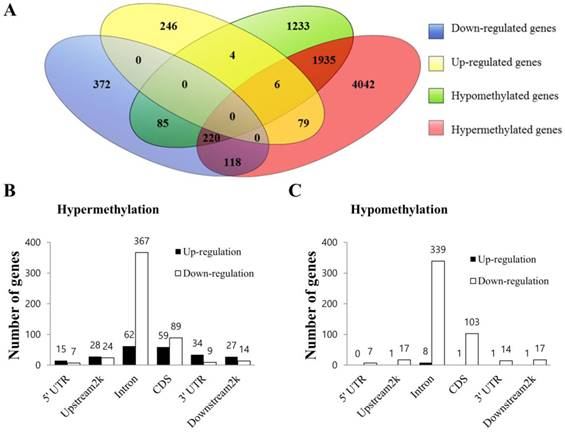
\includegraphics[width=0.8\textwidth]{journal-of-cancer_sample-result}}
%	\caption{یک نمونه نمودار خلاصه برای نمایش نوآوری در نتایج
%		%\cite{kim2016integrated}
%	}
%	\label{fig:sampleDiagram}
%\end{figure}\\
%طبیعتاً به صلاحدید نگارنده، شکل‌ها و نمودار‌ها می توانند در بخش های مختلف، خصوصا فصل
%\ref{chap:results}
%مورد استفاده قرار گیرند.
%
%\subsection{تعریف واژه‌ها (اختیاری)}
%در این قسمت محقق باید واژه‌هایی را که ممکن است برای خواننده آشنا نباشد، تعریف کند.
%
%\subsection{خلاصه فصل‌ها}
%در آخرین قسمتِ فصل اول پایان‌نامه، خلاصه‌ای اشاره‌وار از فصل‌های آتی آورده می‌شود تا خواننده بتواند تصویری واضح از دیگر قسمت‌های پایان‌نامه در ذهن خود ترسیم کند.
%
%\section{جمع‌بندی}
%در این فصل به دو مقولهٔ نحوه استفاده از قالب \پ دانشگاه تهران و نیز ویژگی‌هایی که محتویات فصل اول پایان‌نامه (یعنی مقدمه) باید داشته باشند، پرداخته شد. با توجه به اینکه این راهنما نحوه استفاده از قالب را شرح داده، ملزومات محتوایی هر فصل پایان‌نامه را توضیح می‌دهد و در پیوست‌ها نیز نحوهٔ کار با لاتک را یادآوری خواهد کرد، بنابراین مطالعهٔ کامل آن مقداری وقت شما را خواهد گرفت؛ اما مطمئن باشید از اتلاف وقت شما در ادامه کارتان تا حد زیادی جلوگیری خواهد کرد. در نوشتن متن حاضر سعی شده است علاوه بر ایجاد یک قالب لاتک برای پایان‌نامه‌های دانشگاه تهران، نکات محتوایی هر فصل نیز گوشزد گردد. طبیعتاً برای نگارش پایان‌نامهٔ خود می‌بایست مطالب تمام فصل‌ها را خودتان بازنویسی کنید.
%
%در ادامهٔ این راهنما، تنها فصل‌هایی که یک پایان‌نامه باید داشته باشد و نیز خصوصیات یا ساختاری که محتویات هر فصل باید از آنها برخوردار باشد%
%\footnote{از روی فایل «تمپلیت نگارش و تدوین پایان‌نامه \cite{UTThesisGuide}»}،
%آورده می‌شوند. نهایتاً  در پیوست‌ها، مطالبی در باب یادآوری دستورات لاتک، نحوه نوشتن فرمول‌ها، تعاریف، قضایا، مثال‌ها، درج تصاویر، نمودارها، جداول و الگوریتم‌ها و نیز مدیریت مراجع، آمده است.
%
%همچنین توصیه اکید دارم که رفع خطاهایی که احتمالاً با آنها مواجه می‌شوید را به آخر موکول نفرمایید و به محض برخورد با خطا، آن را اشکال‌زدایی و برطرف نمائید.